\chapter{Common aspects to multi-b+\met SUSY searches}
\label{chap:multib_general}

The main results presented in this thesis are the two analyses described in Chapter \ref{chap:strong_prod} and Chapter \ref{chap:ewk_prod}, which target respectively the strong and electroweak production of supersymmetric particles.
While these analyses target two different benchmark models, they have many commonalities, since both models feature 
a final state rich in $b$-jets and missing transverse momentum (\met). This Chapter highlights these common aspects: 
Section \ref{sec:simplified_models} describes the philosophy of simplified models, used to design and interpret the searches. 
Sections \ref{sec:common_obj_def} and \ref{sec:common_syst} focus on the definition of the physics objects and the experimental systematic uncertainties respectively; Section \ref{sec:common_variables} presents the main kinematic variables used in the analyses 
while Section \ref{sec:common_backgrounds} describes the background sources from \gls{sm} processes, 
how they are modeled in the analyses and the uncertainties on this modelling. 

\section{Simplified models}
\label{sec:simplified_models}

Even with the simplifying assumptions of the \gls{pmssm}, discussed in Section \ref{sec:theory:pmssm}, a \gls{susy} model has to take into account a large number of free parameters, whose values can impact the characteristics of the particle production and decay. 
Simplified models \cite{Alves:2011wf} are very simple models of \gls{bsm} Physics involving only a few particles and decay modes, 
each one focusing on a specific signature, which can be used to optimize and interpret analyses targeting \gls{bsm} scenarios. 
In general simplified models can be viewed as a limit of more complete models, where all particles except a few are too heavy to be 
produced in the interactions. This leads to a drastic reduction of the number of parameters: a simplified model can be described just by the production cross-section and mass of the few particles considered. 
The \glspl{br} of the new particles can be a parameter of the simplified model as well, but it is in general easier to consider each decay chain as a separate simplified model with 100\% \gls{br}.
When simplified models are used to discover or exclude a certain topology, it is important to connect the results obtained to more general models, 
which can be done e.g. by relaxing the restrictions on the \gls{br} of the \gls{bsm} particles or allowing additional particles to take part in the interaction.

\section{Analysis strategy}
\label{sec:analysisstrategy}

The analysis strategy is based on the definition of so-called \glspl{sr}, signal-enriched regions defined by selections on relevant kinematic variables with the goal of maximizing the sensitivity to specific benchmark models. 
After the \glspl{sr} are defined, the key aspect of the analysis is an accurate estimate of the number of events expected from \gls{sm} processes (background events) in these regions, and of the associated uncertainty. 
With the background estimate in hand, it is possible to look at the observed yields in data and compare it with the expectations;
this comparison, performed with the statistical methods discussed in Chapter \ref{chap:stat}, allows quantifying the significance of an excess or placing limits on \gls{bsm} signal models.

The estimate of the expected background events can be performed with different techniques. In particular, in these thesis three types of techniques are used:
\begin{itemize}
\item A first option is to take the background estimate directly from \gls{mc} simulation. 
\item The \gls{mc} estimate can be improved by normalizing each process in a dedicated \gls{cr}, which is a region non overlapping with the \gls{sr}, but kinematically close to it, enriched in the background process that we want to normalize and with a very low expected signal fraction. Since \gls{cr} and \gls{sr} must be non-overlapping, some of the selections of the \gls{sr} are inverted to design the \gls{cr}; the extrapolation of the background normalization factor form the \gls{cr} to the \gls{sr} is tested in dedicated \glspl{vr}. Figure \ref{fig:susy_common:CRschema} shows a schematic view of the relation between \glspl{cr}, \glspl{vr} and \glspl{vr}. A simplified example of how the usage of \glspl{cr} can lead to an improved background prediction with reduced systematic uncertainties is discussed in Section \ref{sec:example_cr}. 
\item In some cases, a background estimate that relies only on data and not on \gls{mc} simulation is preferred. In these cases we speak of a data-driven background estimate.
\end{itemize}

\begin{figure}
\centering
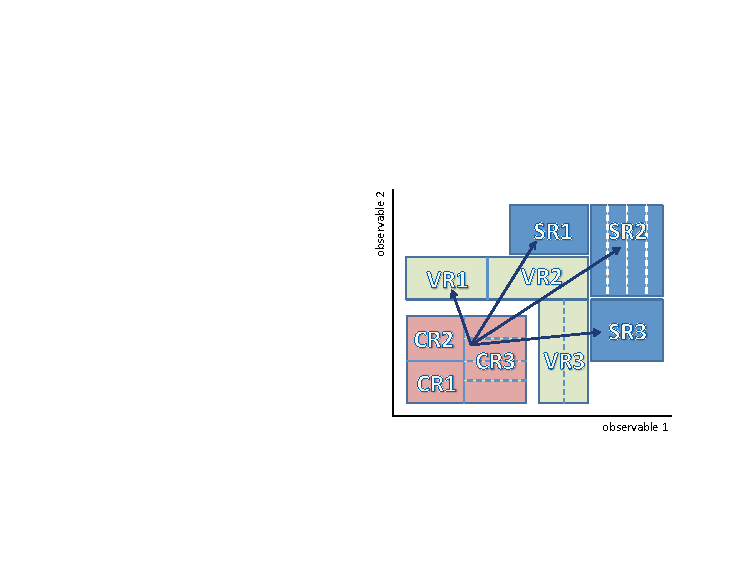
\includegraphics[width=0.55\textwidth]{figures/susy_common/CR_VR}
\caption{Schematic view of the relation between \glspl{cr}, \glspl{vr} and \glspl{vr}. Figure from Ref. \cite{Baak:2014wma}.}
\label{fig:susy_common:CRschema}
\end{figure}
 
In each of the analyses described in this thesis, two different analysis strategies are carried out in parallel:
\begin{description}
\item[Cut-and-count] Several \glspl{sr} are designed, each optimized to maximize the discovery significance to a specific region of the parameter  space, represented by one benchmark model. Cut-and-count \glspl{sr} are useful also to provide simple and powerful model-independent \glspl{ul}, that are easy to re-interpret for signal models different than the ones considered in the analysis. 

\item[Multi-bin] In this case, the \glspl{sr} are non-overlapping. This requirement conflicts with the simple choice of the best selection to maximize the significance, which means that the individual discovery power of each \gls{sr} is smaller than in the case of cut-and-count \glspl{sr}. On the other hand, having non-overlapping \glspl{sr} allows to statistically combine them in the likelihood fit, leading to a stronger model-dependent expected \gls{ul}. The increase in expected exclusion obtained with the combination of several regions is demonstrated in Section \ref{sec:example_combi}.
 
\end{description}


\section{Object definition}
\label{sec:common_obj_def}

Physics objects used in the analyses are defined with two sets of inclusive selections:
a first set of looser selections defines the baseline objects. 
These are used as input for the overlap removal algorithm which, in the steps defined in the next paragraph,
solves the possible double-counting of physics objects (e.g. electrons reconstructed also as jets); objects that survive the overlap removal procedure are then subject to 
tighter selections to define the signal objects. The specific selections applied to jets, electrons and muons are:

\begin{description}

\item[Jets] Baseline jets are reconstructed with the anti-$k_T$ algorithm 
%(described in Section \ref{sec:obj:jetfinding}) 
with radius parameter $R=0.4$ 
and use the calibration procedure discussed in Section \ref{sec:obj:jetcalib}. 
The kinematic selection on baseline candidate jets is  $\pt > 20$ GeV and $|\eta|<2.8$; 
In order to suppress fake jets originating from pileup interactions, jets with $\pt<60$ GeV are required to have \gls{jvt} > 0.59 and satisfy the cleaning criteria discussed in Section \ref{sec:jetcleaning} with the \textit{BadLoose} \gls{op}.
After overlap removal, signal jets are required to have $\pt>30 (20)$ GeV for the analysis discussed in Chapter \ref{chap:strong_prod} (\ref{chap:ewk_prod}); the difference on the \pt threshold 
in the two analyses is related to differences in the signal event kinematics, and will be discussed more in detail in the specific chapters.

Jets are considered $b$-tagged based on the output of the MV2c10 algorithm (see Section \ref{sec:btagging}); in both analyses the \gls{op} used corresponds to an average efficiency of 77\% for $b$-jets from simulated  
\ttbar events, and to a rejection factor of 6, 22 and 134 against jets originating from $c$-quarks, hadronic decays of $\tau$ leptons and light jets respectively. 


\item[Re-clustered jets] Baseline jets that survive the overlap removal are re-clustered with the anti-$k_T$ algorithm into large-R jets of radius $R=0.4$, as described in Section \ref{sec:reclustering}. 
Re-clustered jets are trimmed removing the constituents whose \pt falls below 10\% of the \pt of the re-clustered jet, and are then required to have $\pt>100$ GeV and $|\eta|<2.0$.

\item[Electrons] Baseline electrons have to satisfy the Loose identification \gls{op} (see Section \ref{sec:elec_id}) and required to have $\pt > 20 (5)$ GeV the analysis discussed in Chapter \ref{chap:strong_prod} (\ref{chap:ewk_prod}) and $|\eta|<2.47$. 
After overlap removal, signal electrons are required to satisfy the Tight identification \gls{op} and the $LooseTrackOnly$ isolation \gls{op}, and  to have $\pt > 20$ GeV.
Electrons are matched to the \gls{pv} by requiring $|\dzero/\sigma_\dzero| < 5$ and  $|\zzerost| < 0.5$ mm.


\item[Muons] Baseline muons are required to satisfy the Medium identification \gls{op} (see Section \ref{sec:muon_id}) and to have $\pt > 20 (5)$ GeV in the analysis discussed in Chapter \ref{chap:strong_prod} (\ref{chap:ewk_prod}) and $|\eta|<2.5$. 
After overlap removal, signal muons are required to satisfy the $LooseTrackOnly$ isolation \gls{op} and to have $\pt > 20$ GeV.
Muons are also matched to the \gls{pv} by requiring $|\dzero/\sigma_\dzero| < 3$ and  $|\zzerost| < 0.5$ mm; muons that do not satisfy this selection as considered as cosmic muons, and the events with at least one cosmic muons are vetoed.

\end{description}

The missing transverse momentum is defined considering all the calibrated objects in the event, as described in Section \ref{sec:met}, and uses the \gls{tst} to account for the contribution of
detector signals not associated to reconstructed objects. 

\subsubsection*{Overlap removal}

Potential overlaps between jets, electrons and muons are resolved sequentially with the overlap removal procedure. 
First of all, electrons that are likely to originate form muon bremsstrahlung, i.e. those that lie within $\dR < 0.01$ from a muon candidate, are removed.

Overlaps between jet candidates and electron arise mostly from two reasons. Electrons are reconstructed from deposits in the calorimeter, and are therefore reconstructed as jets as well.
In this case we want to preserve the electron and remove the jet, so we remove any non-$b$-tagged jet that lies within $\dR < 0.2$ from an electron candidate;
an exception is done for $b$-tagged jets, since in this case the electron is likely to originate from a semileptonic $B$-hadron decay. 
Electron candidates that are close to the surviving jets are likely to have been produced in the decay of an hadron inside the jet, and are therefore removed
if they lie within $\dR<0.4$ from a jet and their energy is lower than 50 GeV, or if their energy is higher than 50 GeV and the \dR from the jet 
is lower than min$(0.4, 0.04 + 10 \, {\rm{GeV}}/E_{\rm{T}})$. 
Having an energy-dependent \dR selection aims at increasing the acceptance for leptons originating from the decay of boosted top quarks.

Unlike electrons, muons are unlikely to be reconstructed as jets. Therefore, the first step in the overlap removal procedure between muon candidates and jets 
aims primarily at removing the muons that originate from the decay of hadrons inside the jets. 
Muons and jets can also be close if the jet is originating from muon bremsstrahlung; these jets typically have a small number of associated \gls{id} tracks.
Therefore jets that lie within $\dR < 0.2$ from a muon are removed if they are not $b$-tagged and if they have less than three matching \gls{id} tracks. 
Muons in close proximity to the surviving jets are removed 
if they lie within $\dR<0.4$ from a jet and their \pt is lower than 50 GeV, or if their \pt is higher than 50 GeV and the \dR from the jet 
is lower than min$(0.4, 0.04 + 10 \, {\rm{GeV}}/\pt)$. 

\section{Experimental systematic uncertainties}
\label{sec:common_syst}

Each of the selections in the definition of the objects described in Section \ref{sec:common_obj_def} has an associated experimental systematic uncertainty on the modelling of that selection in 
the \gls{mc} simulation. The experimental systematic uncertainties that are most relevant for analyses targeting final states with multiple $b$-jets and \met are:

\begin{description}

\item[JES and JER] As discussed in Section \ref{sec:obj:jetcalib}, the \gls{jes} and \gls{jer} calibration procedures allow to both calibrate the jet energy from the \gls{em} to the
hadronic scale, and also to correct \gls{mc} simulations to describe better the data; the uncertainties on these corrections propagate to the analyses. 
For the \gls{jes}, reduced sets of uncertainties are available that reduce the number of \glspl{np} to be included in the analysis at the cost of potential loss in correlation; 
the analyses discussed in this thesis use a strongly reduced set with three \glspl{np}. 
Uncertainties on \gls{jes} and \gls{jer} are the leading source of experimental uncertainties, as they can change the kinematic of the jets in the event, and therefore also the number
of jets that fulfill certain selections.

\item[$b$-tagging] The uncertainties on the $b$-tagging calibration procedure (see Section \ref{sec:obj:btaggingcalib}) are included through uncertainties on the $b$-tagging \gls{sf}. 
They are divided into one \gls{np} for the uncertainty on the efficiency of tagging jets originating from $b$-quarks, 
one for the mistagging of the jets originating from 
$c$-quarks, and one for light jets; 
furthermore, one additional \gls{np} for the high-\pt extrapolation uncertainty, based on MC simulation studies, 
increases the uncertainties in the high-\pt region, where the $b$-tagging calibration is not available and the central 
value of the \gls{sf} is taken from the closest calibrated \pt region. 
The uncertainties on $b$-tagging play a relevant role in the analyses in this thesis, as they rely heavily on the selection of events containing $b$-tagged jets.

\item[Luminosity] Besides those uncertainties associated with the object selections, 
another experimental uncertainty that is taken into account in the analysis is 
the uncertainty on the integrated luminosity, whose measurement is described in Section \ref{sec:lumimeas}; for the 2015-2016 dataset the luminosity uncertainty corresponds 
to 3.2\% and is derived with a strategy similar to that described in Ref. \cite{Aaboud:2016hhf}. The impact of this uncertainty on the analyses discussed in this thesis is very small.

\end{description}

\noindent The following systematic uncertainties have been explicitly tested to be negligible in the analyses and are therefore not included in the final results presented in this thesis:

\begin{description}
\item[Leptons] The uncertainties on the calibration and resolution of the energy (momentum) of electrons (muons).
% have been tested to be negligible in all the analyses discussed in this thesis. 

\item[\met] The three \glspl{np} that take into
account the uncertainty on the scale and the parallel and perpendicular resolution of the \met soft term. 
Note that, while the \met soft term uncertainties are not included in the final results, 
the propagation of the \gls{jes} and \gls{jer} uncertainties to the \met computation 
are always properly taken into account.

\end{description}


\section{Common kinematic variables}
\label{sec:common_variables}

The kinematic properties of the objects in the event are used to define variables that, by combining information about multiple objects, 
provide a handle to discriminate between the signal evens from the benchmark model being tested, and the background events from \gls{sm} processes, described in Section \ref{sec:common_backgrounds}. 
While a few of these variables are related to specific characteristics of the signal model, especially in the case of the Higgsino search 
discussed in Chapter \ref{chap:ewk_prod} that involves two Higgs bosons, most of them are built based on the features of the main  
background processes we need to suppress and are therefore in common between the two analyses. 

\subsubsection*{Object energy and multiplicity}

Even just the multiplicity of the objects defined in Section \ref{sec:common_obj_def} provides a powerful handle to analyze the characteristics of an event. In particular, the following multiplicity variables are used:

\begin{description}
\item[\njet] Number of signal jets in the event.
\item[\nbjet] Number of signal jets that are $b$-tagged using the 77\% \gls{op}.
\item[\nlep] Number of signal leptons (electrons and muons) in the event.
\end{description}

\noindent In addition to multiplicity variables, we can also use the energy of the individual objects as a discriminating variable; 
for example, we always consider events with a minimum \met of 200 GeV (the selection is tighter in some \glspl{sr}), 
or we can consider only jets with \pt above a certain threshold if we expect high-\pt jets from the signal. 

\subsubsection*{Effective mass}

The effective mass is defined as the scalar sum of the momenta of all the signal objects in the event and the missing transverse momentum:

\begin{equation}
\meffi = \sum_{i\leq n} {\pt}^{j_i}  + \sum_{j\leq m} {\pt}^{\ell_j}  + \met \; .
\end{equation}

\noindent This variable reflects the overall energy scale of the event, and in the signal is therefore correlated to the mass of the \gls{susy} particles produced. 

\subsubsection*{Transverse mass}

The transverse mass between lepton and \met (\mt) is defined for events with at least one selected signal lepton as: 

\begin{equation}
\mt = \sqrt{2\pt^{\rm{lep}}\met(1-\cos\Delta\phi(\met,\pt^{\rm{lep}}))} \; ,
\end{equation}

\noindent where $\pt^{\rm{lep}}$ is the transverse momentum of the leading signal lepton in the event. 
For events where this lepton and the entire \met derive from the decay of a parent particle with mass m$_{\rm{parent}}$, \mt presents an endpoint at m$_{\rm{parent}}$. 
This is the case when the lepton and \met derive form the leptonic decay of a $W$ boson, in $W$+jets events or in semileptonic \ttbar events; 
note that dileptonic \ttbar events do not present the same endpoint at the W-boson mass, as it is not possible to completely disentangle the energy of the two neutrinos. Events from W+jets or semileptonic \ttbar processes can have values of \mt higher than the kinematic endpoint only if some of the objects in the event are not properly reconstructed (e.g. fake \met from mismeasured jets, jets misidentified as leptons, or leptons out of acceptance).

Another variable useful to suppress the \ttbar background is the minimum transverse mass between \met and the $b$-jets in the event:

\begin{equation}
\label{eq:mtbmin}
\mtb =  \mathrm{min}_{i\leq 3}  \sqrt{(\met+p_T^{j_i})^2 - ({\met}_x+p_x^{j_i})^2 - ({\met}_y+p_y^{j_i})^2 } \; ,
\end{equation}

\noindent where the minimum is taken over the transverse mass computed with the three leading $b$-tagged jets in the event. 
In semileptonic \ttbar events, this variable presents an endpoint near the top-quark mass, as this is the endpoint that we would have if \met originating from the neutrino is perfectly measured and the $b$-jet produced in the decay of the same top quark as the neutrino is among the three leading $b$-tagged jets. 


\subsubsection*{Multijet suppression}

\gls{sm} background events without any neutrino in the decay chain can still have a sizable amount of reconstructed \met if one of the jets in the 
event is mismeasured, leading to a fake energy imbalance in the event. In these cases, the resulting \met will have a value of the azimuthal angle ($\phi$) close to the one of the mismeasured jet. The variable \dphimin is defined as the minimum difference in azimuthal angle between \met and the  four jets with the highest \pt in the event:

\begin{equation}
\dphimin = \textrm{min}_{i \leq 4}(|\phi_{{\rm{jet},}i} - \phi_{\met}|) \; .
\end{equation}

\noindent Requiring high values of this variable helps rejecting events with no real \met. 


\section{Background processes and their modelling}
\label{sec:common_backgrounds}

This section describes the main background processes in the analysis regions, 
which are characterized by the selection of events with an high number of $b$-jets and high \met, and the way they are modeled. 
In general, the modelling is based on \gls{mc} simulations for
all the backgrounds, except multijet which is estimated with a data-driven technique.
For the main background, pair production of top quark pairs (\ttbar), the shape of the different distributions is obtained from \gls{mc}
but the normalization is data-driven, derived in specifically designed \glspl{cr} and tested in \glspl{vr} as described in Section \ref{sec:analysisstrategy}.

\begin{figure}[h]
\centering 
\subfigure[]{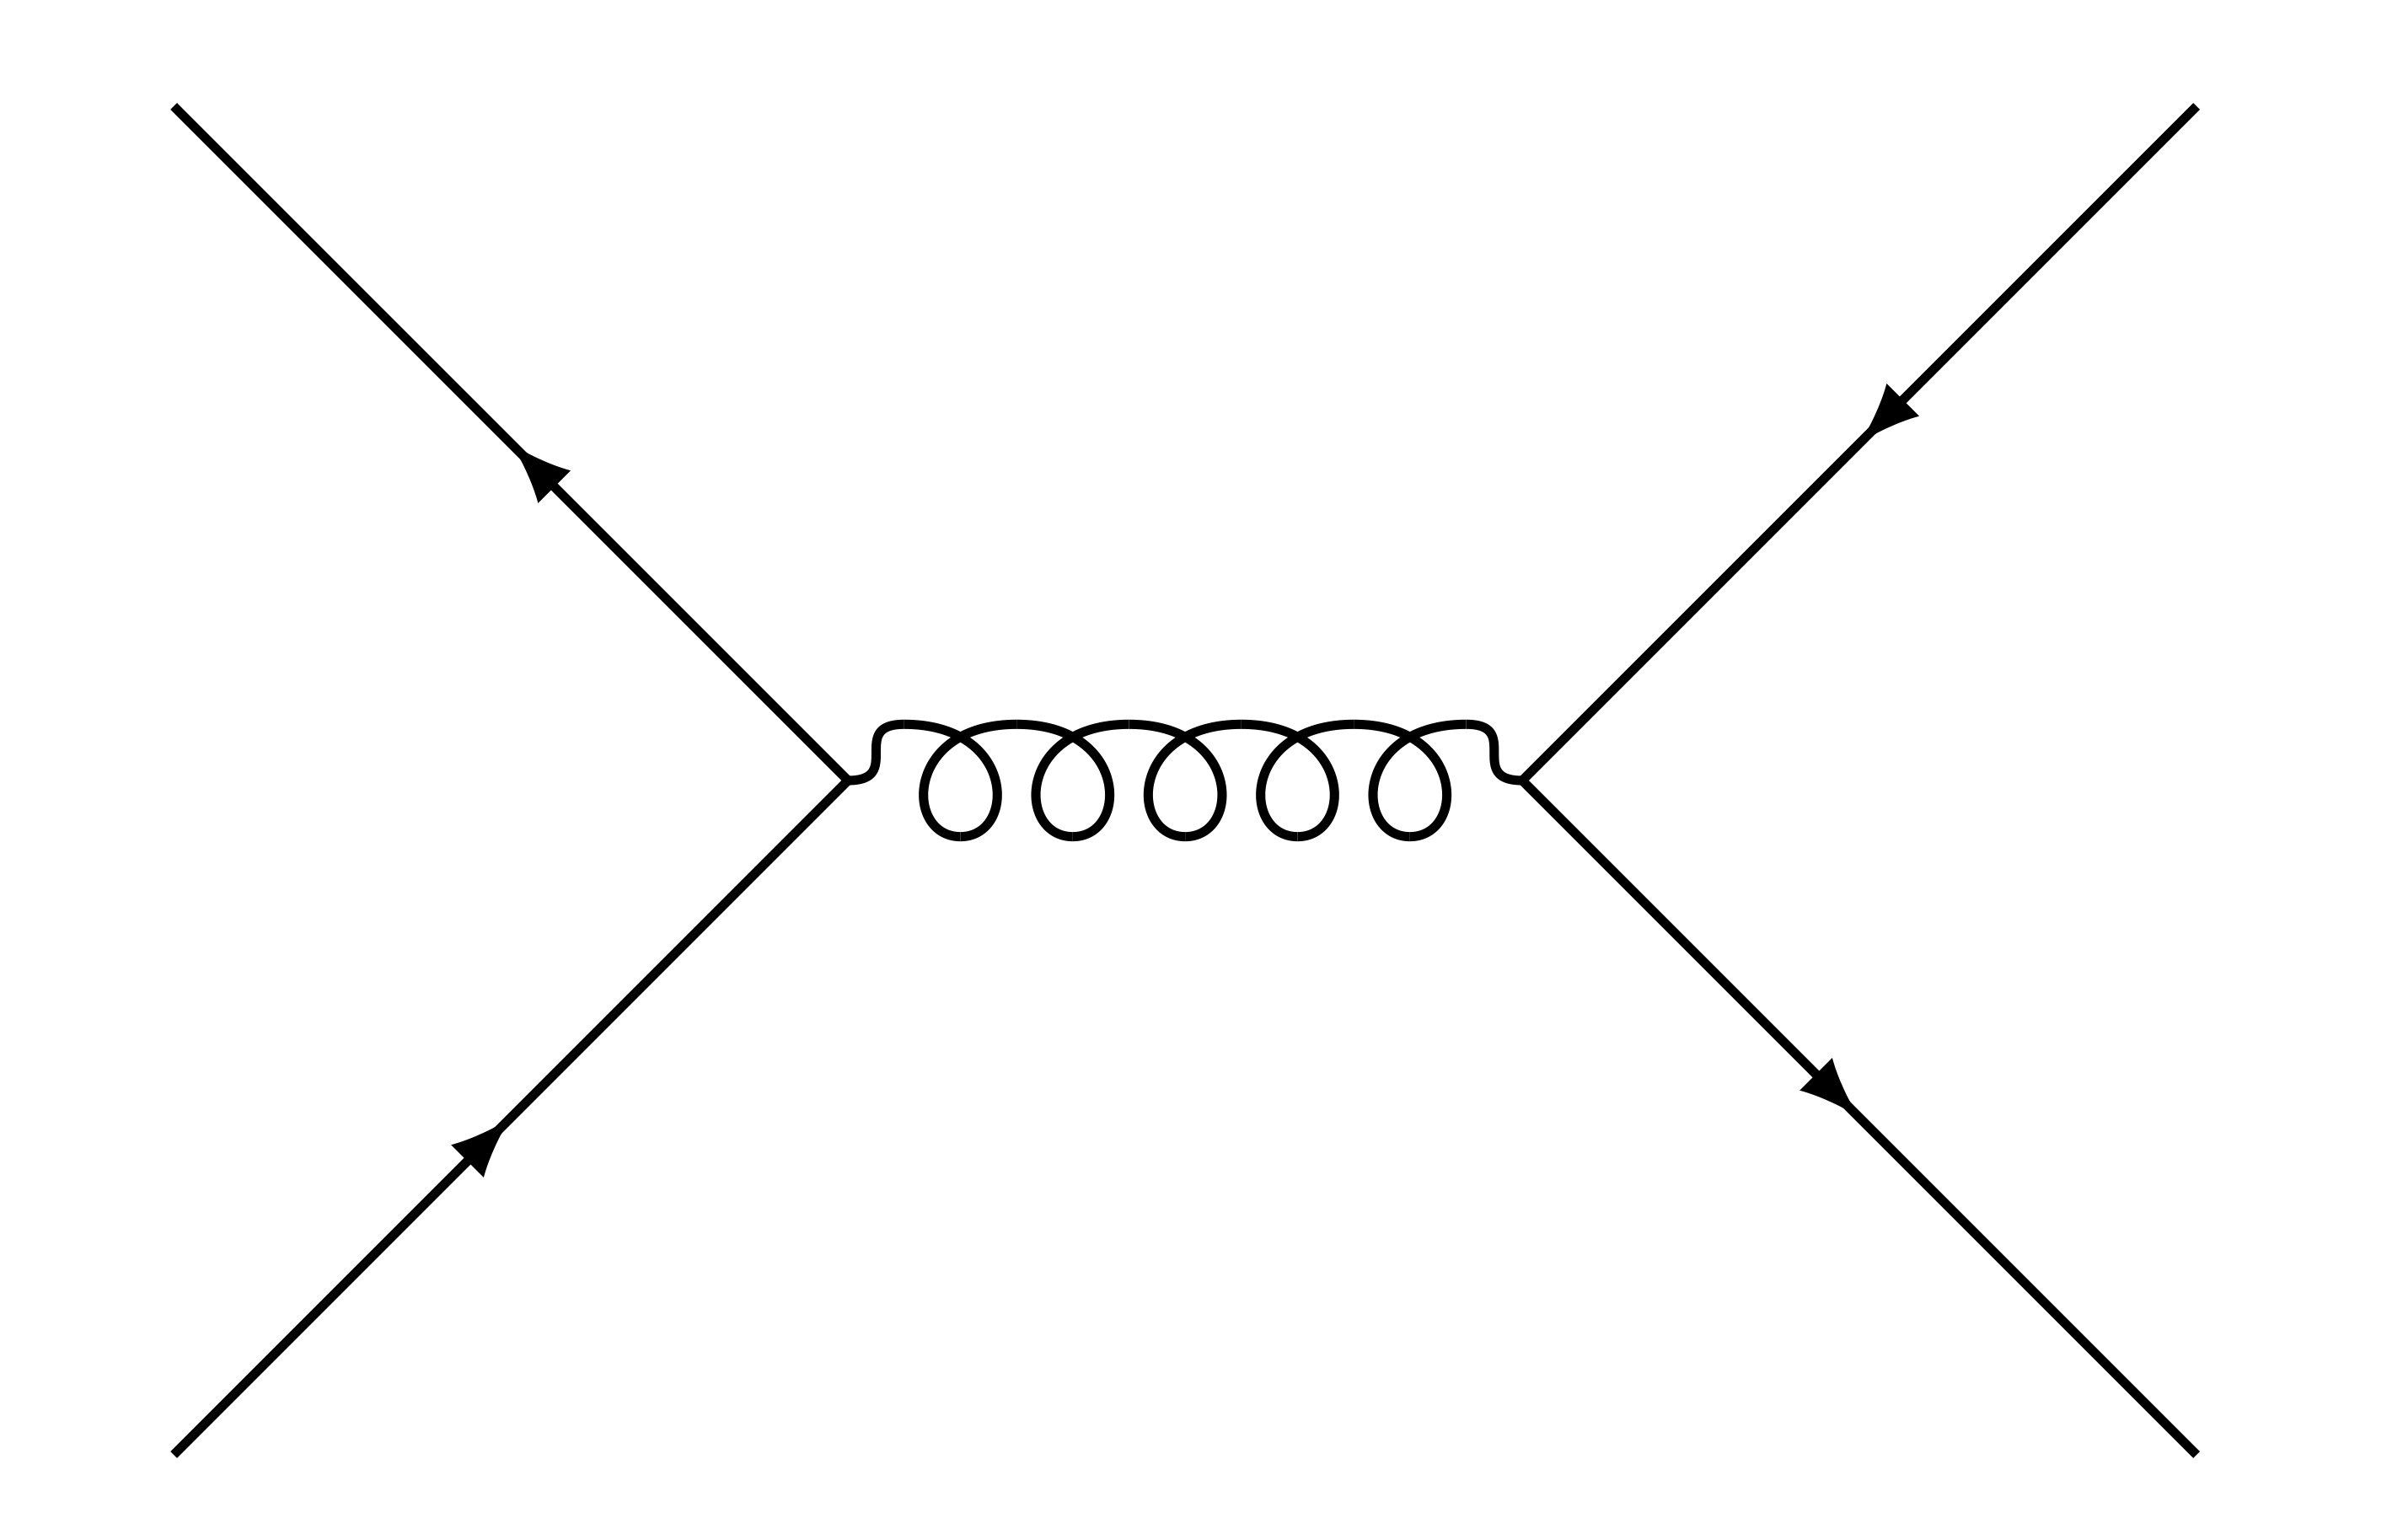
\includegraphics[width=0.3\textwidth]{figures/susy_common/feynman/ttbar_4}\label{fig:ttbar_prod_qq}}\\
\subfigure[]{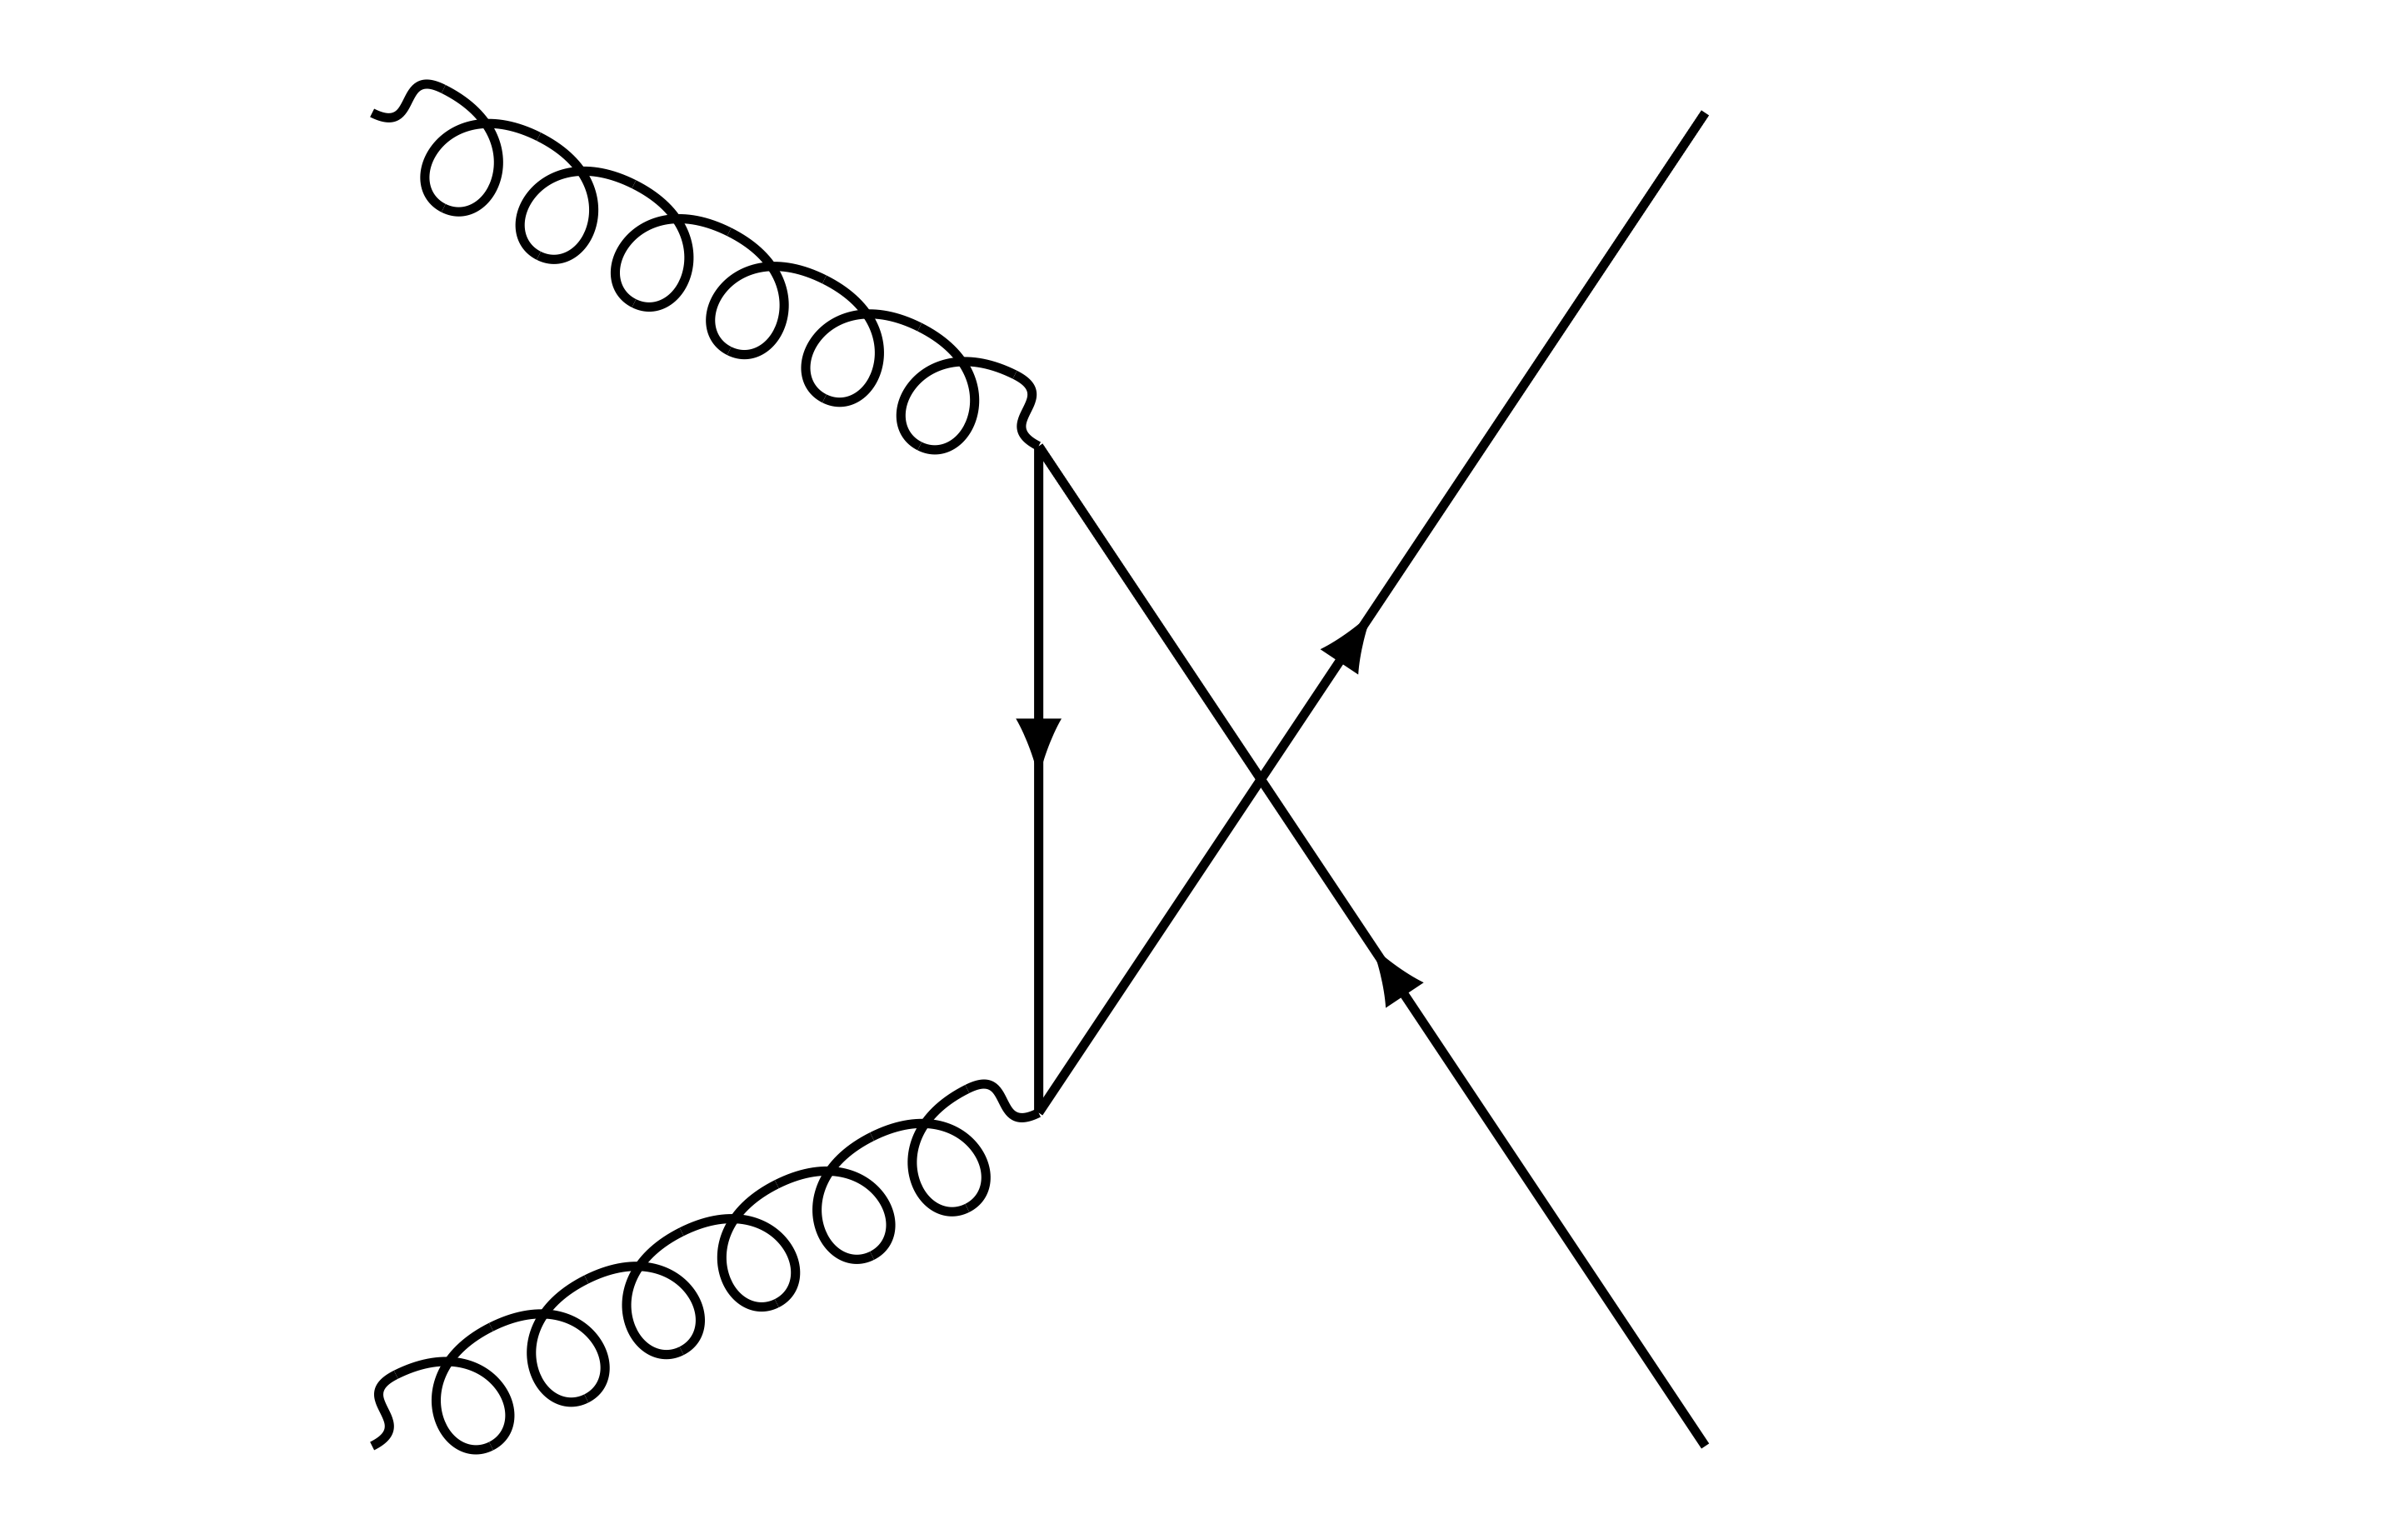
\includegraphics[width=0.3\textwidth]{figures/susy_common/feynman/ttbar_1}\label{fig:ttbar_prod_gg_1}}
\subfigure[]{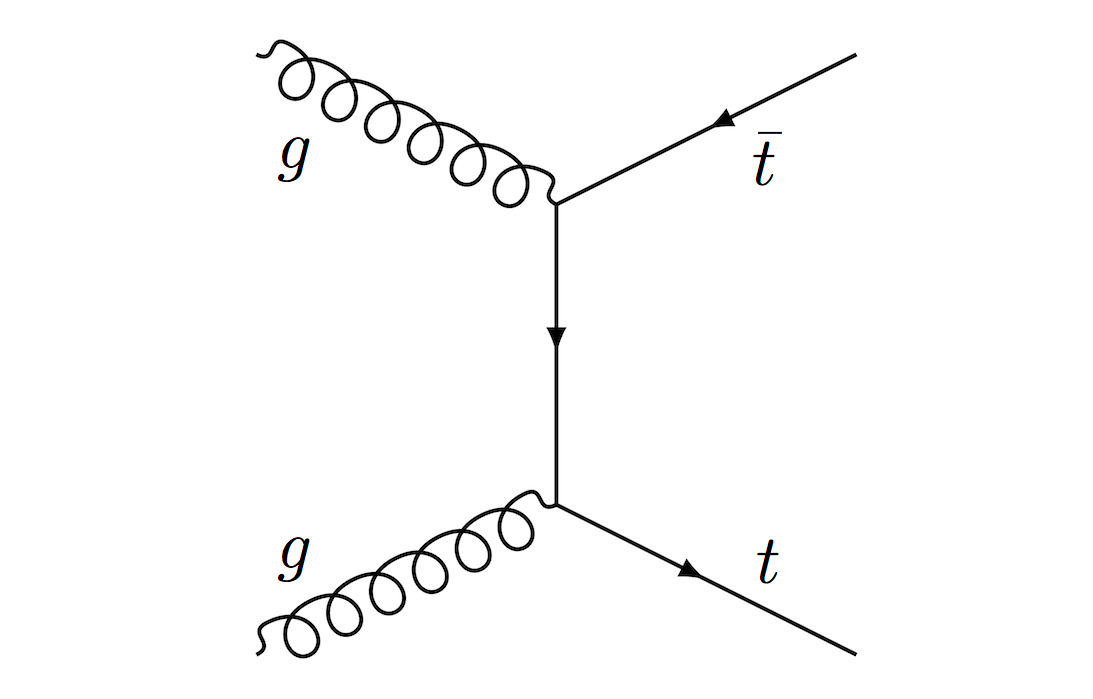
\includegraphics[width=0.3\textwidth]{figures/susy_common/feynman/ttbar_3}\label{fig:ttbar_prod_gg_2}}
\subfigure[]{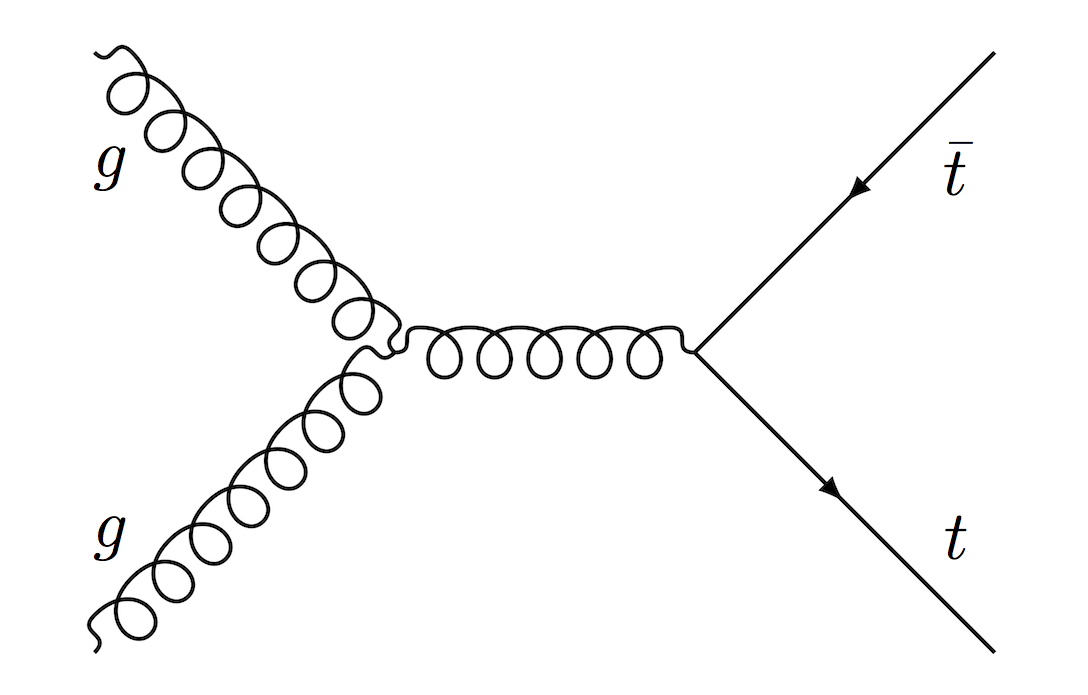
\includegraphics[width=0.3\textwidth]{figures/susy_common/feynman/ttbar_2}\label{fig:ttbar_prod_gg_3}}
\caption{\Gls{lo} Feynman diagram for the production of top quark pairs initiated by \subref{fig:ttbar_prod_qq} quark-antiquark annihilation and \subref{fig:ttbar_prod_gg_1}-\subref{fig:ttbar_prod_gg_3} gluon-gluon fusion.}\label{fig:ttbar_prod}
\end{figure}

\subsection{Top quark pair production}
\label{sec:susy_general:ttbar}

Given the presence of several $b$-jets in the final state, \ttbar production in association with jets constitutes the main source of \gls{sm} background in all the analysis regions. \ttbar production, which at the \gls{lhc} at 13 TeV has a cross-section of $831.8^{+19.8 + 35.1}_{-29.2-35.1}$ pb \cite{Czakon:2013goa}, is mediated by the strong interaction, and it can occur through quark-antiquark annihilation (Fig. \ref{fig:ttbar_prod_qq}) or through gluon-gluon fusion (Fig. \ref{fig:ttbar_prod_gg_1} to \ref{fig:ttbar_prod_gg_3}). When the \gls{lhc} is running at 13 TeV, the threshold fraction of the proton energy that must be carried by each parton in order to have sufficient energy to produce a system of two top quarks 
is about 2.6\%.
%, assuming a top quark mass of 173.1 GeV \cite{Patrignani:2016xqp}. 
At these low fractions, the \gls{partdf} of the gluon is higher than the \gls{partdf} of quarks and much higher than the \gls{partdf} of the antiquarks, so gluon-gluon fusion is the dominant \ttbar production mode at the \gls{lhc}.


In the \gls{sm}, the top quark decays $\approx 99.8$\% of the times to a $W$ boson and a $b$-quark. 
Beside the pair of $b$-quarks, which are always present, the final state can be characterized based on the decay of the two $W$ bosons, leading to three different categories:
\begin{description}
\item[Dilepton]  Both $W$ bosons decay to a lepton ($e$, $\mu$, $\tau$) and a neutrino (10.5\%).
\item[Single-lepton] One $W$ boson decays to lepton and neutrino, the other decays hadronically (43.8\%).
\item[All-hadronic] Both $W$ bosons decay hadronically (45.7\%).
\end{description}

All the analysis regions considered in this thesis have a tight \met selection (the loosest one is $\met > 200$ GeV). Since the all-hadronic component 
of the \ttbar background does not have any neutrino in the final state, it does not fulfill the \met requirement unless one or more jets are mismeasured; 
this case produces a negligible background in the analysis regions, and is anyway included in the multijet estimate with the jet-smearing method described in Section \ref{sec:jet_smearing}.
The \ttbar components that is dominating the background estimate are the dilepton and single-lepton ones, both in the analysis regions that require reconstructed leptons as well as in the analysis regions that have a lepton veto.
In the second case, the dominating component is the single-lepton component, where one lepton is a hadronically decaying $\tau$, has a \pt too low to be reconstructed, or falls out of acceptance. 
The \gls{mc} generator used to simulate \ttbar events produced in association with high-\pt jets is \PowhegBox v2 with the CT10 \gls{partdf} set \cite{Lai:2010vv} and interfaced with \PY v6.428 \cite{Sjostrand:2006za} for the \gls{psh} and hadronization. 
The normalization is derived in \glspl{cr} designed to be kinematically as close as possible to the corresponding \glspl{sr} (while being non-overlapping with them by inverting some of the selections), and is expressed in terms of \glspl{sf} relative to the cross-section computed with the highest
available accuracy (NNLO+NNLL \cite{Czakon:2011xx}).

\subsubsection*{Truth-level classification: \ttbar decays}

When considering events at particle level,
the \gls{mc} information can be used to reconstruct the decay chains that lead to the stable particles in the final state. 
Starting from each top quark in the event, it is possible to follow its decay chain and classify the event first of all into dilepton or single-lepton, or also with a finer classification based on the flavor of the lepton. 
Subsequent decays of the $\tau$ lepton are not considered, and hadronically decaying $\tau$ leptons are fully considered as leptons in this classification. 
Figure \ref{fig:ttbar_decay_mT_1L} shows the \ttbar decay type as a function of the \mt value  in a selection requiring at least four jets, at least three $b$-jets, $\met>200$ GeV and at least one signal lepton. It is possible to see that, while at low \mt values the \ttbar component is dominated by events where one top quark decays leptonically and the other one decays hadronically, after the kinematic threshold imposed by the mass of the $W$ boson the dilepton component is dominant. 

\begin{figure}[h!]
\centering 
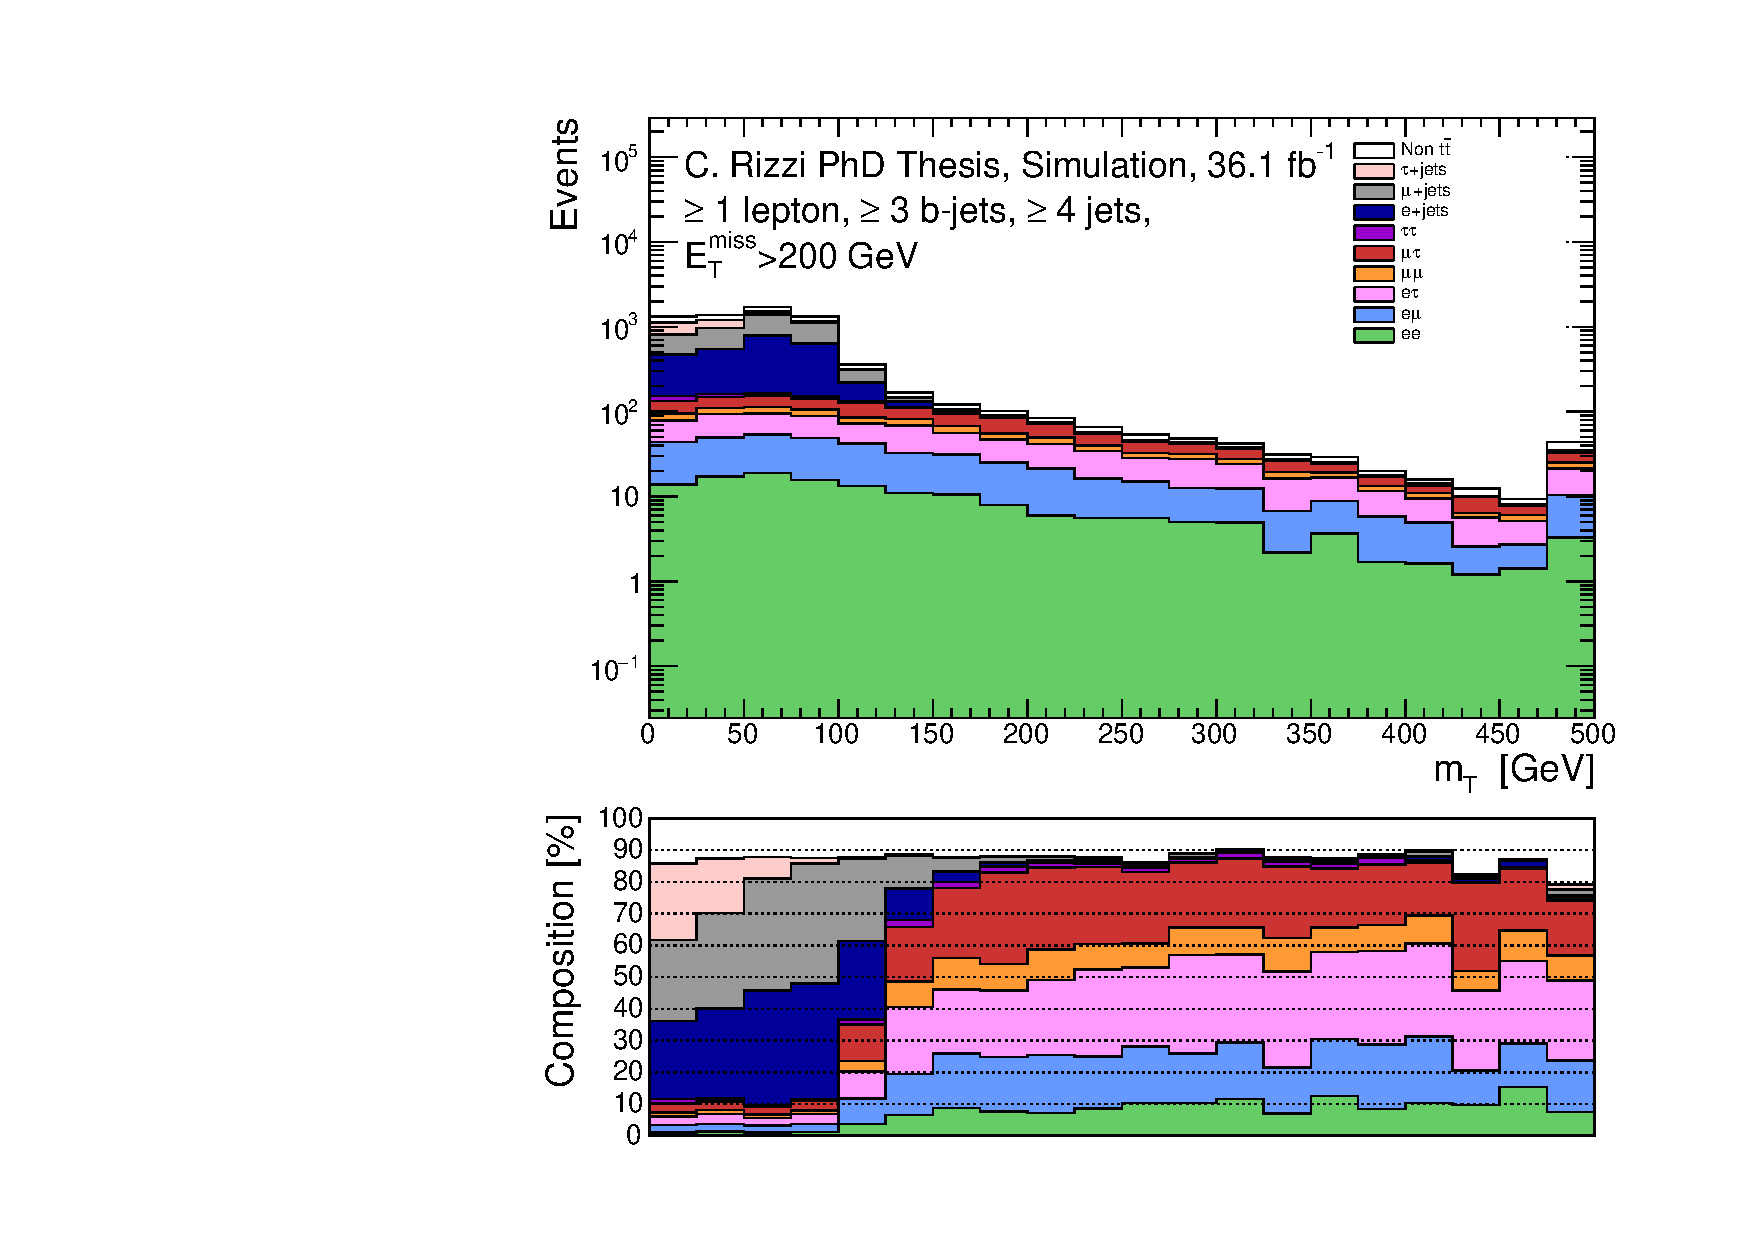
\includegraphics[width=0.49\textwidth]{figures/susy_common/mc_stack_mT_1L_3b_tt_dec.pdf}
\caption{\ttbar decay type as a function of the \mt value  in a selection requiring at least four jets, at least three $b$-jets, $\met>200$ GeV and at least one signal lepton.}\label{fig:ttbar_decay_mT_1L}

\subfigure[]{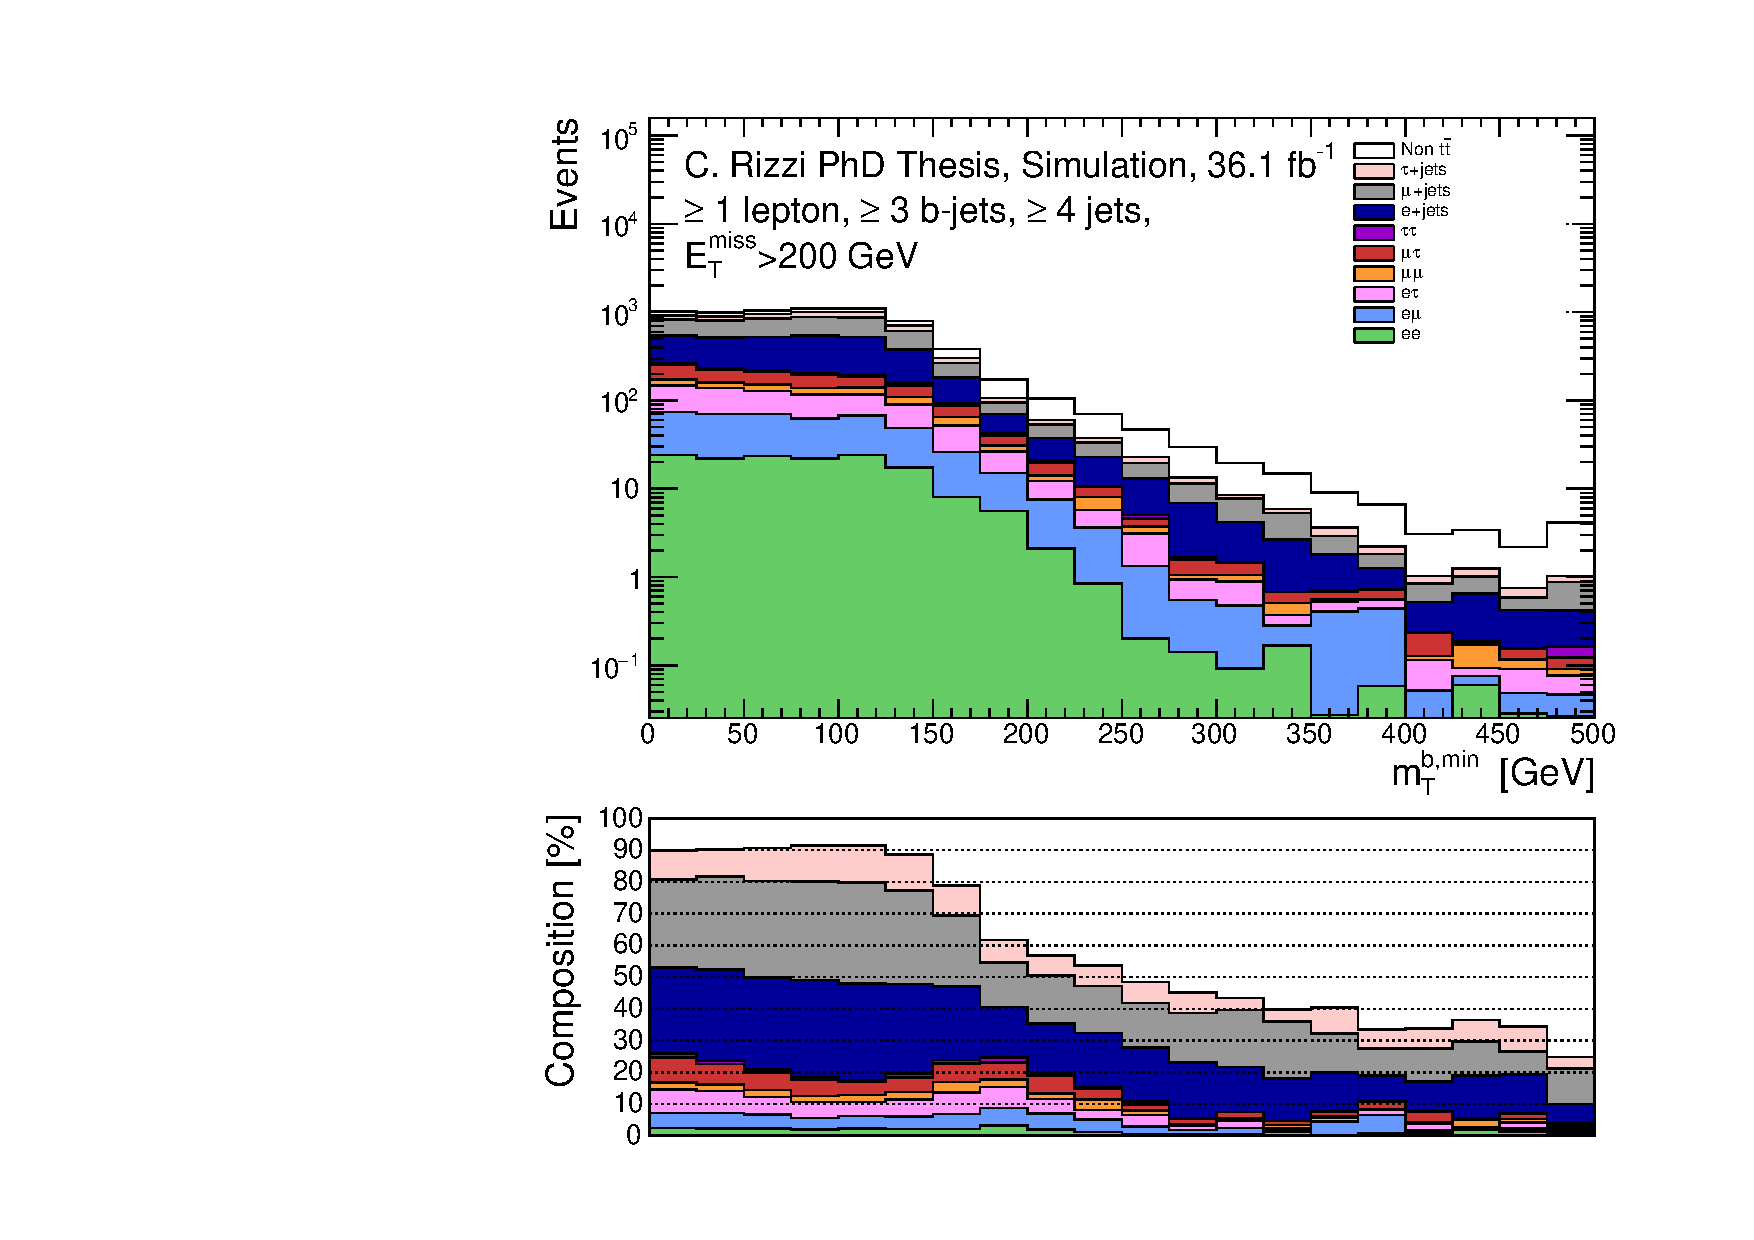
\includegraphics[width=0.49\textwidth]{figures/susy_common/mc_stack_mTb_min_1L_3b_tt_dec.pdf}\label{fig:ttbar_dec_mTb_min_1L}}
\subfigure[]{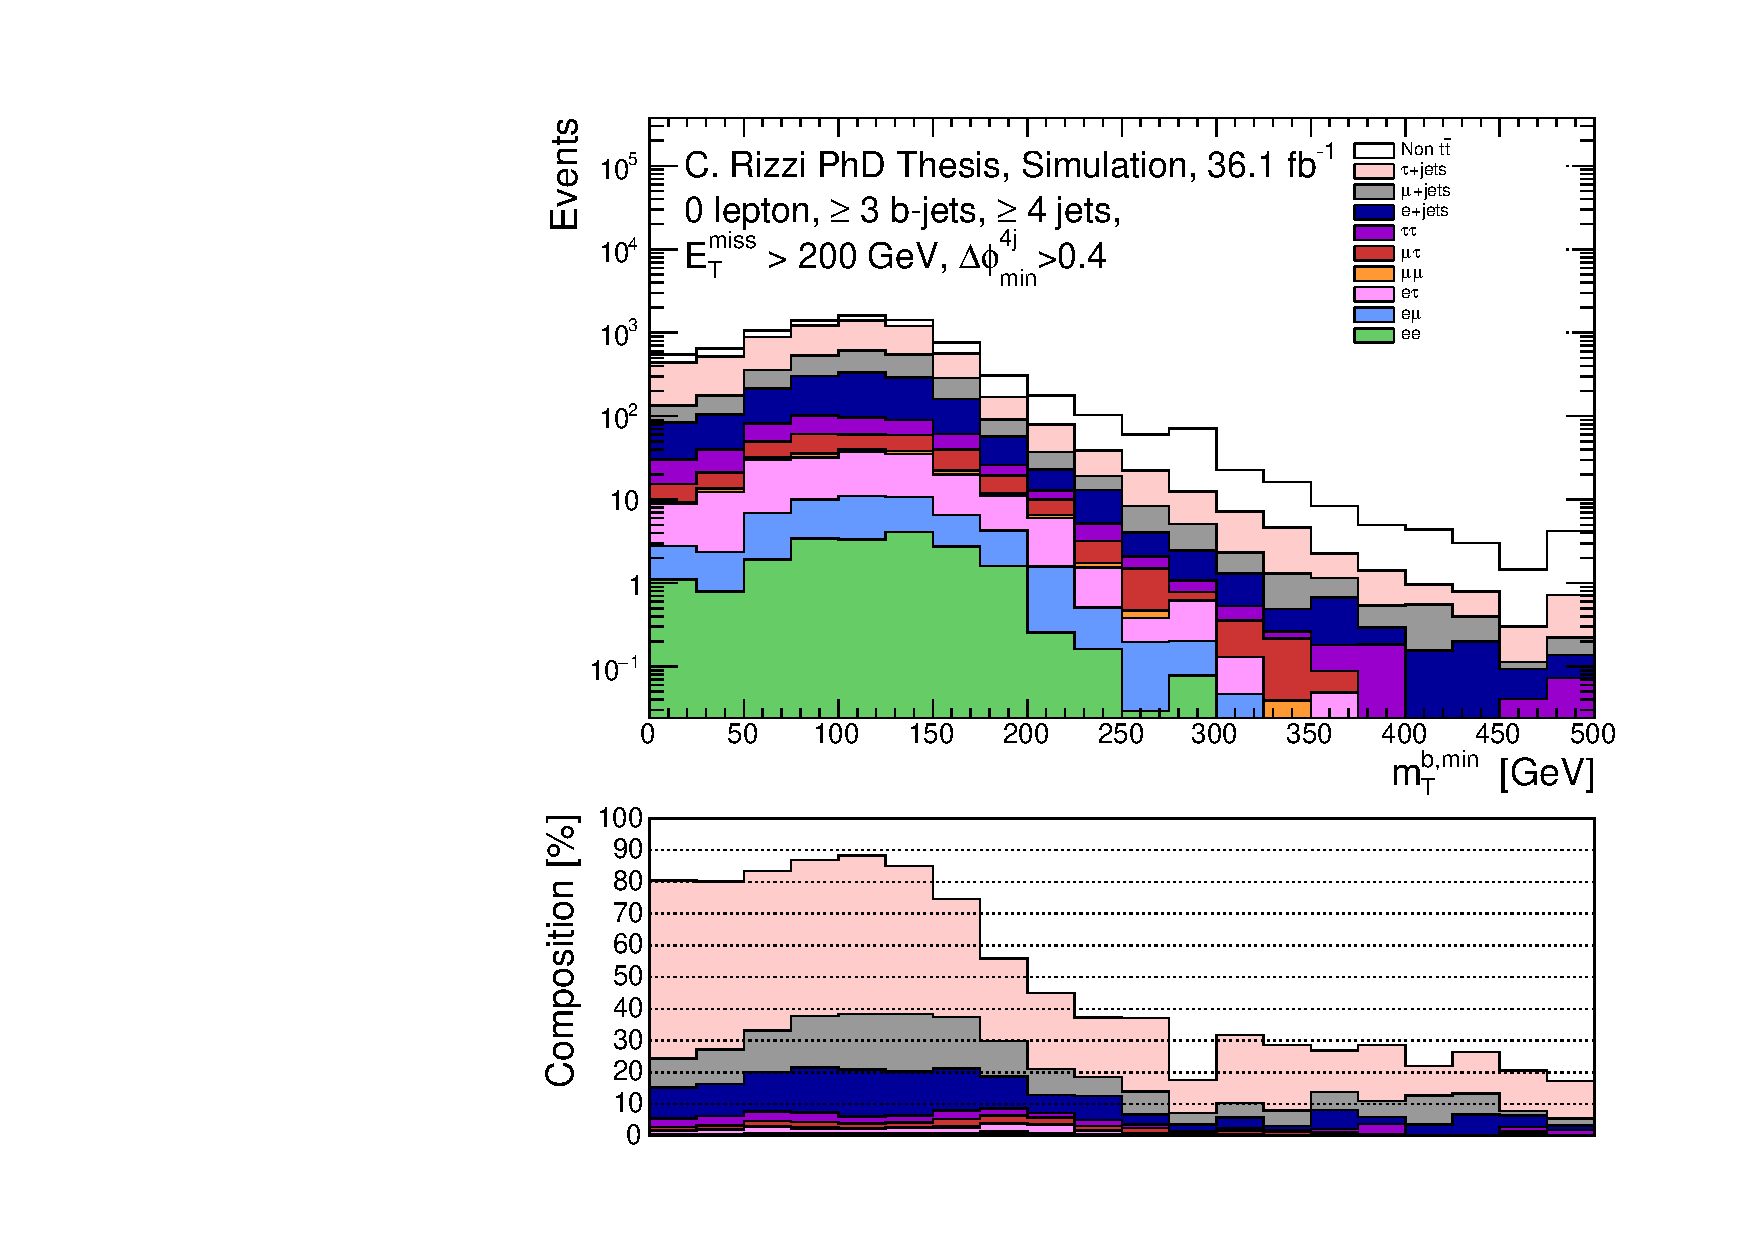
\includegraphics[width=0.49\textwidth]{figures/susy_common/mc_stack_mTb_min_0L_3b_tt_dec.pdf}\label{fig:ttbar_dec_mTb_min_0L}}
\caption{\ttbar decay type as a function of the \mtb value  in a selection requiring at least four jets, at least three $b$-jets, $\met>200$ GeV and \subref{fig:ttbar_dec_mTb_min_1L} at least one signal lepton \subref{fig:ttbar_dec_mTb_min_0L} exactly zero lepton and $\dphimin > 0.4$.}\label{fig:ttbar_decay_mTb_min}
\end{figure}

Figure \ref{fig:ttbar_decay_mTb_min} shows the same \ttbar classification but as a function of \mtb, both in a selection with at least one signal lepton (Figure \ref{fig:ttbar_dec_mTb_min_1L}) and with a lepton veto (Figure \ref{fig:ttbar_dec_mTb_min_0L}). Here it is possible to notice two features. First of all, in general both the selection with a lepton requirement and the one with a lepton veto are dominated by semileptonic decays: in the case of the selection with the lepton requirement the lepton is in most of the cases a muon or an electron, while in the case of the selection with the lepton veto most of the events contain one $\tau$ lepton, which can decay hadronically giving rise to a topology with no electrons or muons.
Secondly, while in the case of \mt \ttbar events are dominating the background composition also for high values of this variable (just with a change from semileptonic to dileptonic \ttbar events), in the case of \mtb after the kinematic endpoint the \ttbar fraction decreases noticeably. 

%\begin{figure}[htb]
%\centering 

%\end{figure}


\subsubsection*{Truth-level classification: flavor of the associated jets}

A truth-level classification is in place to study the \ttbar+jets background based on the flavor of the associated jets.
This is done starting from the \gls{mc} information at particle level; stable particles are grouped into jets using the anti-k$_t$ algorithm 
described in Section \ref{sec:obj:jetfinding} with R=0.4; only particle jets with $\pt > 15$ GeV and $|\eta|<2.5$ are considered. 
The flavor of the jets is determined by matching them with the $B$- and $D$-hadrons that are in a cone of $\Delta R = 0.4$ from the jet. 
If the event contains at least one jet matched to one or more $B$-hadrons, excluding the ones originating from the decay of the top quarks, the event 
is classified as \ttbb. Otherwise, if at least one jet is matched to $D$-hadrons, excluding the ones from the decay chain of the top quarks, the event is classified as \ttcc. \ttbb and \ttcc events are categorized together as \tthf events, where HF stands for heavy flavor, while the remaining ones are classified as \ttlight.
Figure \ref{fig:ttbar_HF_bjets} shows the evolution of the flavor composition of the jets produced in association with \ttbar
as a function of the number of $b$-jets in the event. 
As expected, as the number of $b$-jets increases, the \ttlight fraction decreases and the \ttbb fraction increases. 

\begin{figure}[htb]
\centering 
\subfigure[]{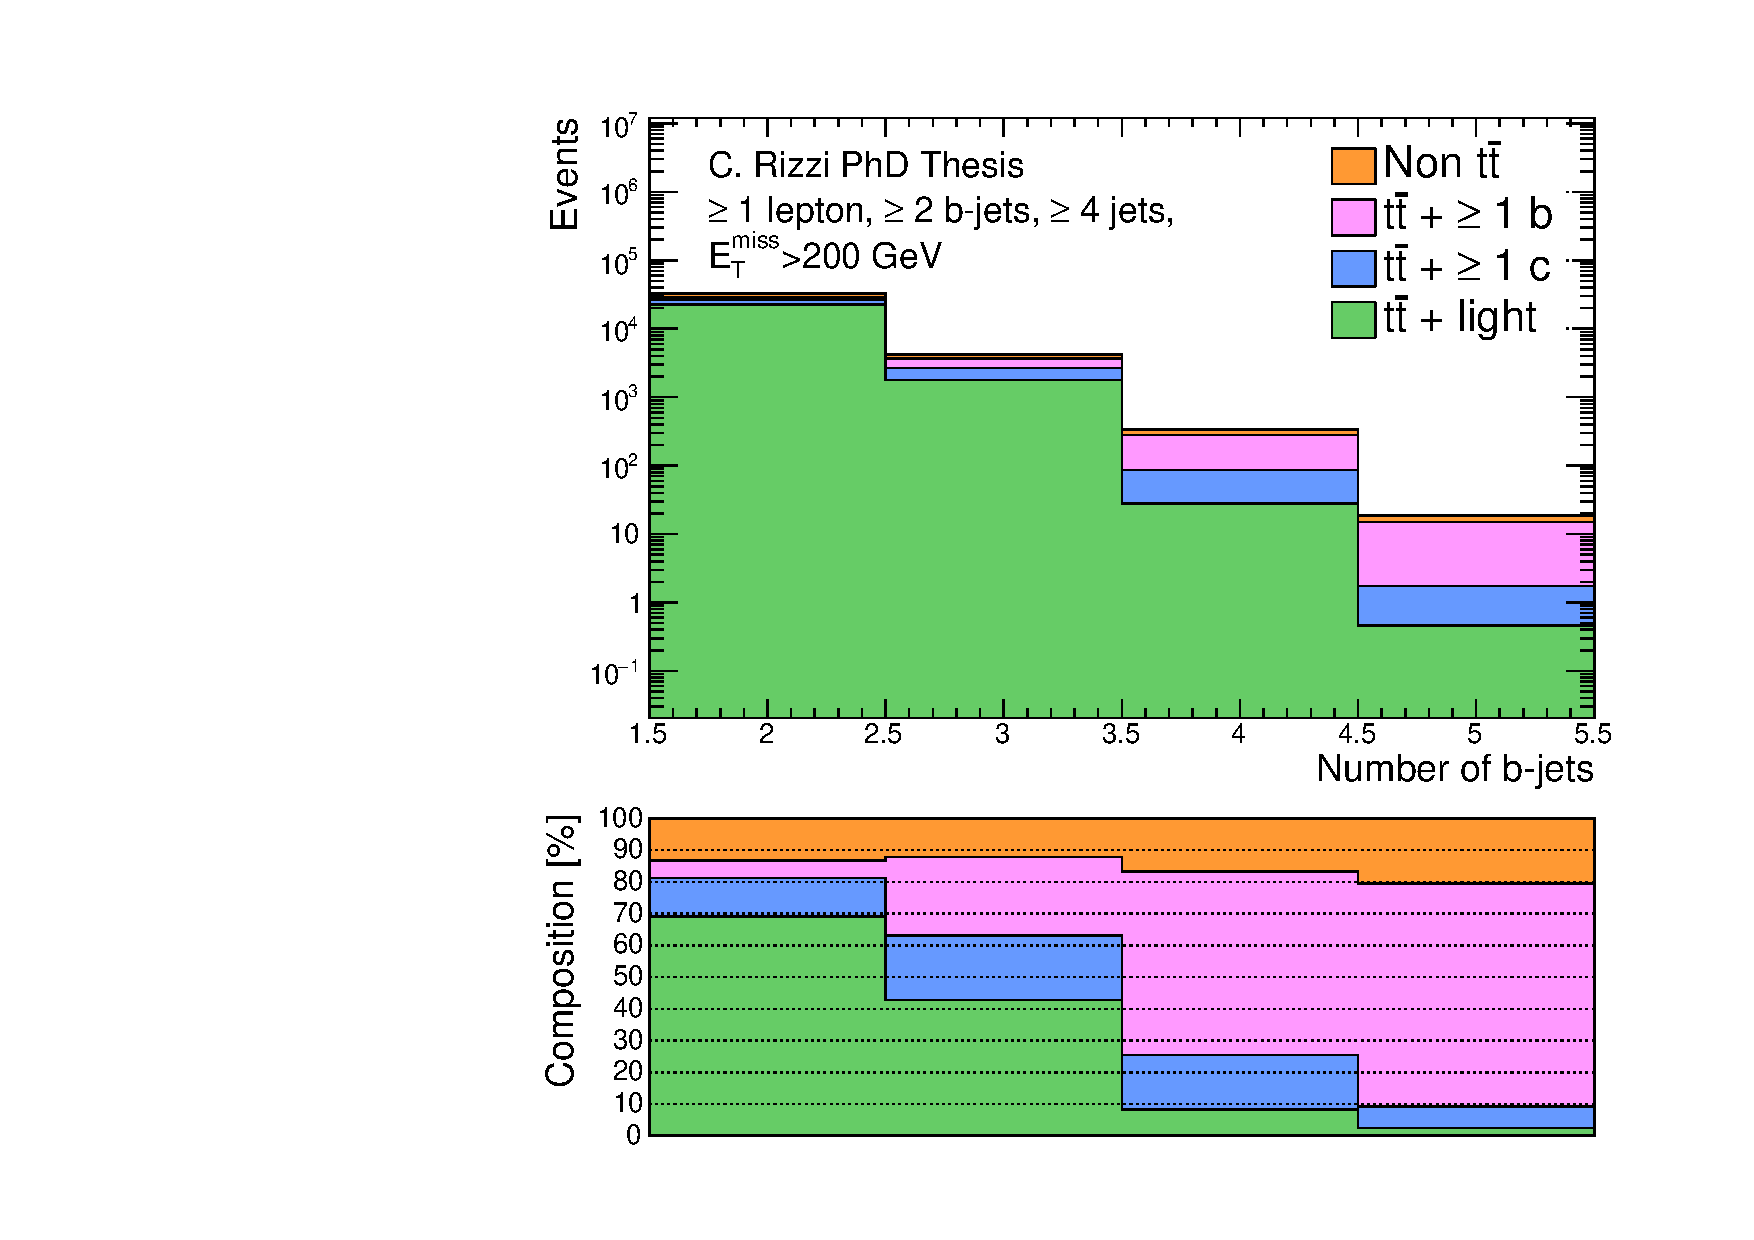
\includegraphics[width=0.49\textwidth]{figures/susy_common/mc_stack_bjets_n_1L_2b_HF.pdf}\label{fig:ttbar_HF_bjets_1L}}
\subfigure[]{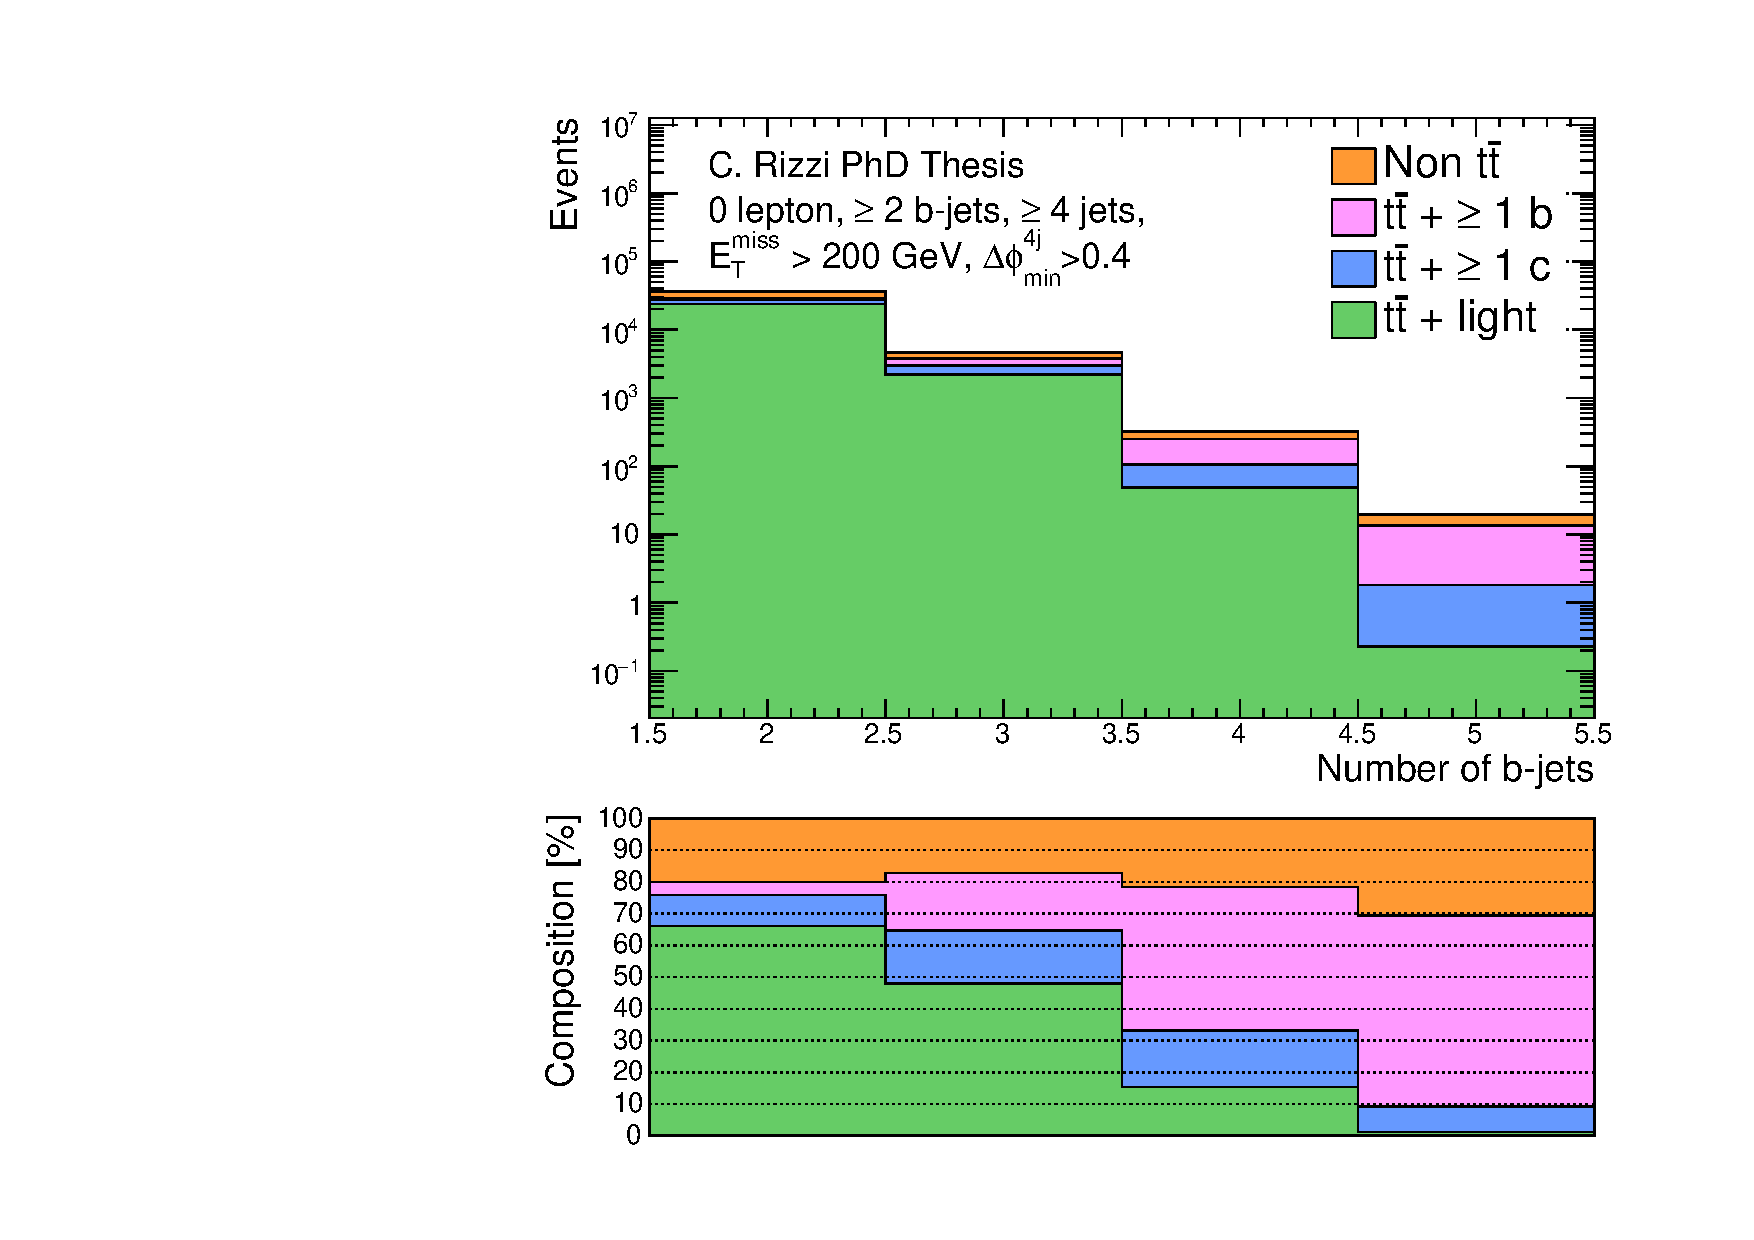
\includegraphics[width=0.49\textwidth]{figures/susy_common/mc_stack_bjets_n_0L_2b_HF.pdf}\label{fig:ttbar_HF_bjets_0L}}
\caption{Evolution of the flavor of the jets produced in association with \ttbar in a selection requiring at least four jets, at least two $b$-jets, $\met>200$ GeV and \subref{fig:ttbar_HF_bjets_1L} at least one signal lepton \subref{fig:ttbar_HF_bjets_0L} exactly zero lepton and $\dphimin > 0.4$.}\label{fig:ttbar_HF_bjets}
\end{figure}


\subsubsection*{Modelling uncertainties}

The modelling uncertainties on the \ttbar background considered in this thesis are:
\begin{description}
\item[Generator] The uncertainty associated with the choice of a specific \gls{mc} generator is estimated by comparing \PowhegBox with \aNLO, both interfaced with \HWpp v2.7.1 with the UEEE5 underlying-event tune.

\item[Parton shower and hadronization] Also the choice of the generator that emulates the \gls{psh} and the hadronization is associated to an uncertainty, that is evaluated by comparing the nominal sample, generated with \PowhegBox and showered with \PY, to another sample generated again with \PowhegBox but showered with \HWpp v2.7.1. 

\item[Radiation] The systematic uncertainty related to the modelling of the \gls{isr} and \gls{fsr} is estimated by comparing samples
generated with \PowhegBox interfaced with two versions of \PY v6.428 with two different settings \cite{Skands:2010ak}. 
One uses the PERUGIA2012radHi tune, has $h_{\rm{dump}}$ parameter set to twice the top mass and the renormalization and factorization scales set to twice the nominal value; these settings lead to an overall larger amount of radiation. The second sample uses a version of \PY with the PERUGIA2012radLo tune, has $h_{\rm{dump}}$ set to the top mass and the renormalization and factorization scales set to half of the nominal value, leading to a description of the event with less additional jets.

\end{description}

Figures \ref{fig:ttbar_nj_0L_syst} and \ref{fig:ttbar_ptj1_0L_syst} show the changes in shape in the distribution of the number of signal jets and the \pt of the leading jet when comparing these systematic variations in a representative selection with a lepton veto.
The normalization of \ttbar events is derived in the \glspl{cr}, therefore modelling uncertainties affect only the extrapolation from 
the \gls{cr} to the corresponding \glspl{sr} and \glspl{vr}, and not the overall normalization. 
The modelling uncertainties are therefore estimated by comparing the expected values for the \glspl{tf}, defined in Section \ref{sec:example_cr}.
as the ratio of expected yields in the \gls{sr} or \gls{vr} over the expected yields in the corresponding \gls{cr}. 
The uncertainties on the \glspl{tf} obtained from the different sources listed above are summed in quadrature in each region, and are treated as uncorrelated across regions to avoid 
constraints from the fit. 


\begin{figure}[htb]
\centering 
\subfigure[]{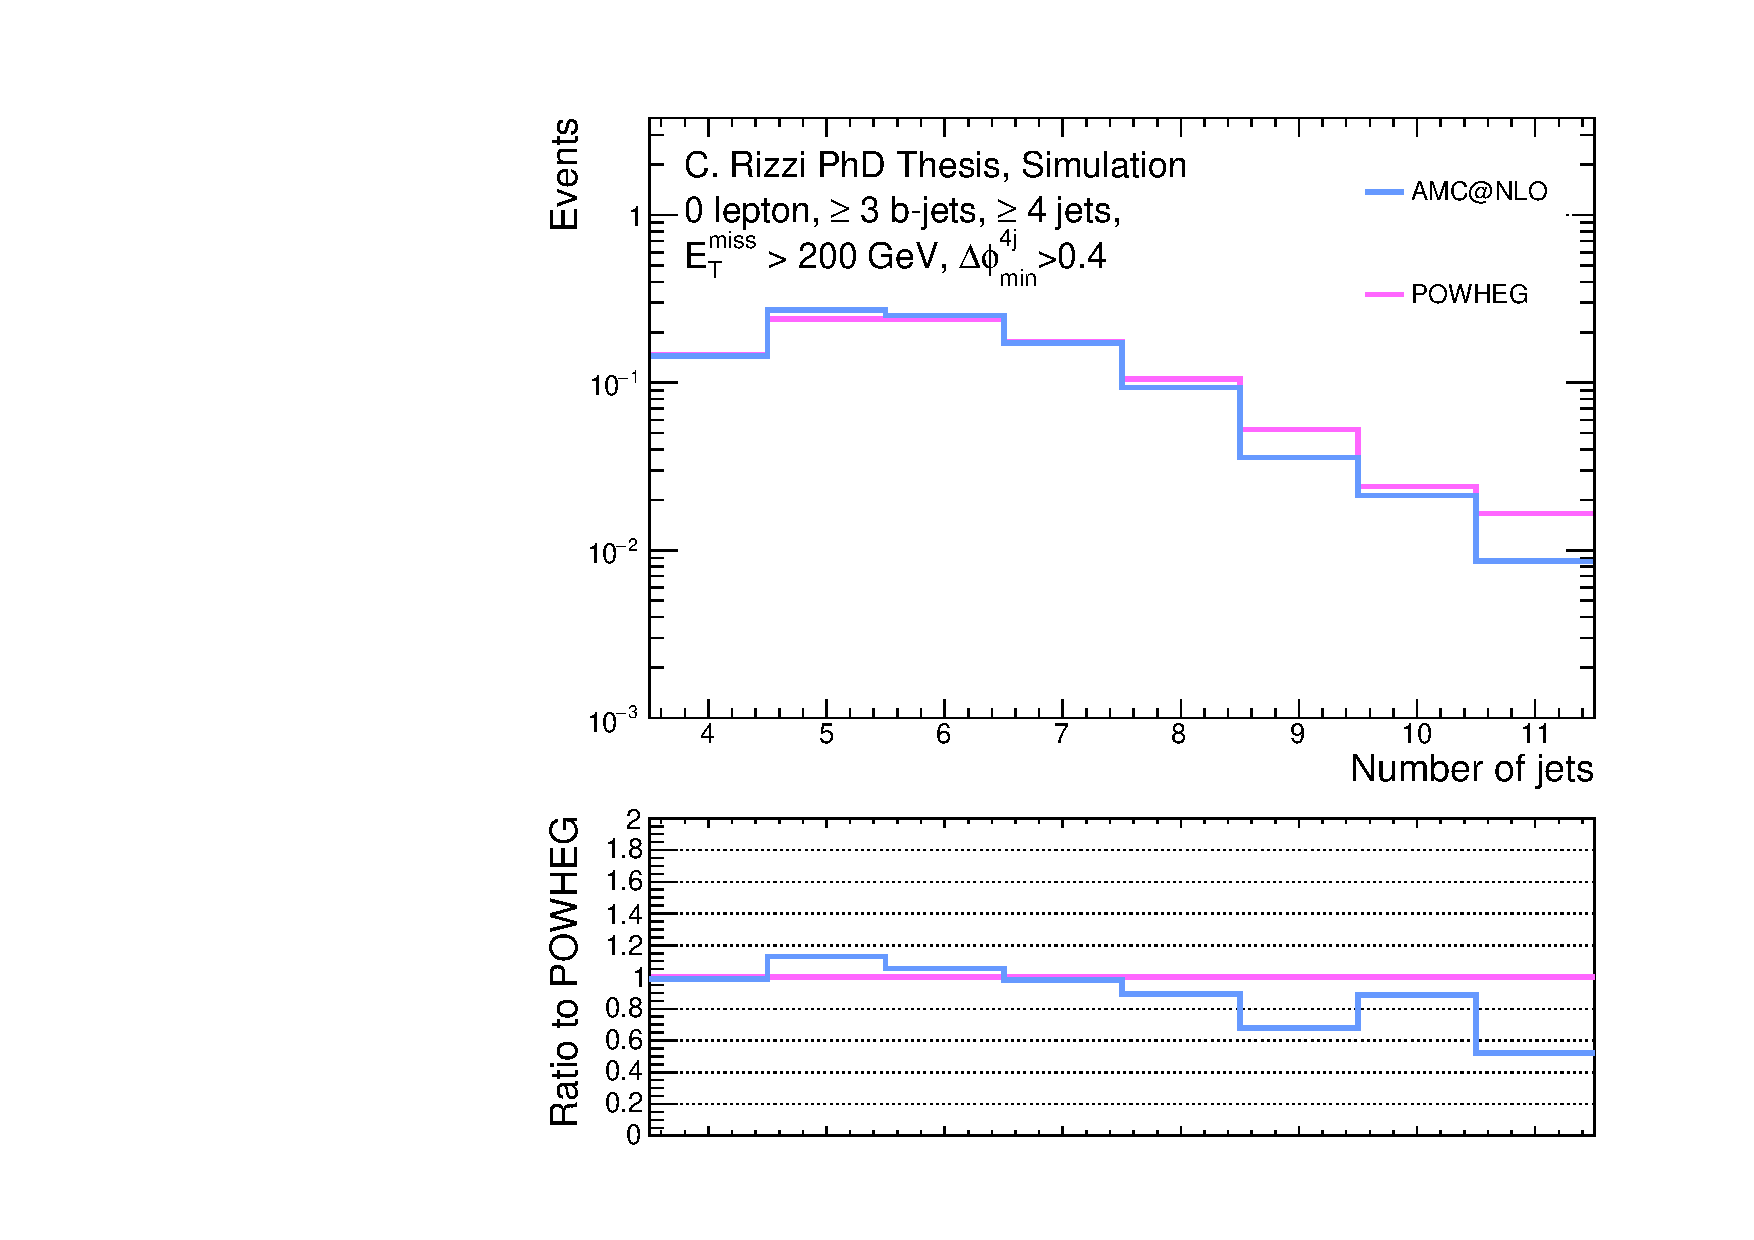
\includegraphics[width=0.32\textwidth]{figures/susy_common/ttbar_syst_gen/0L_3b/compare_jets_n_ttbar_syst_3b_scale.pdf}\label{fig:ttbar_nj_0L_gen}}
\subfigure[]{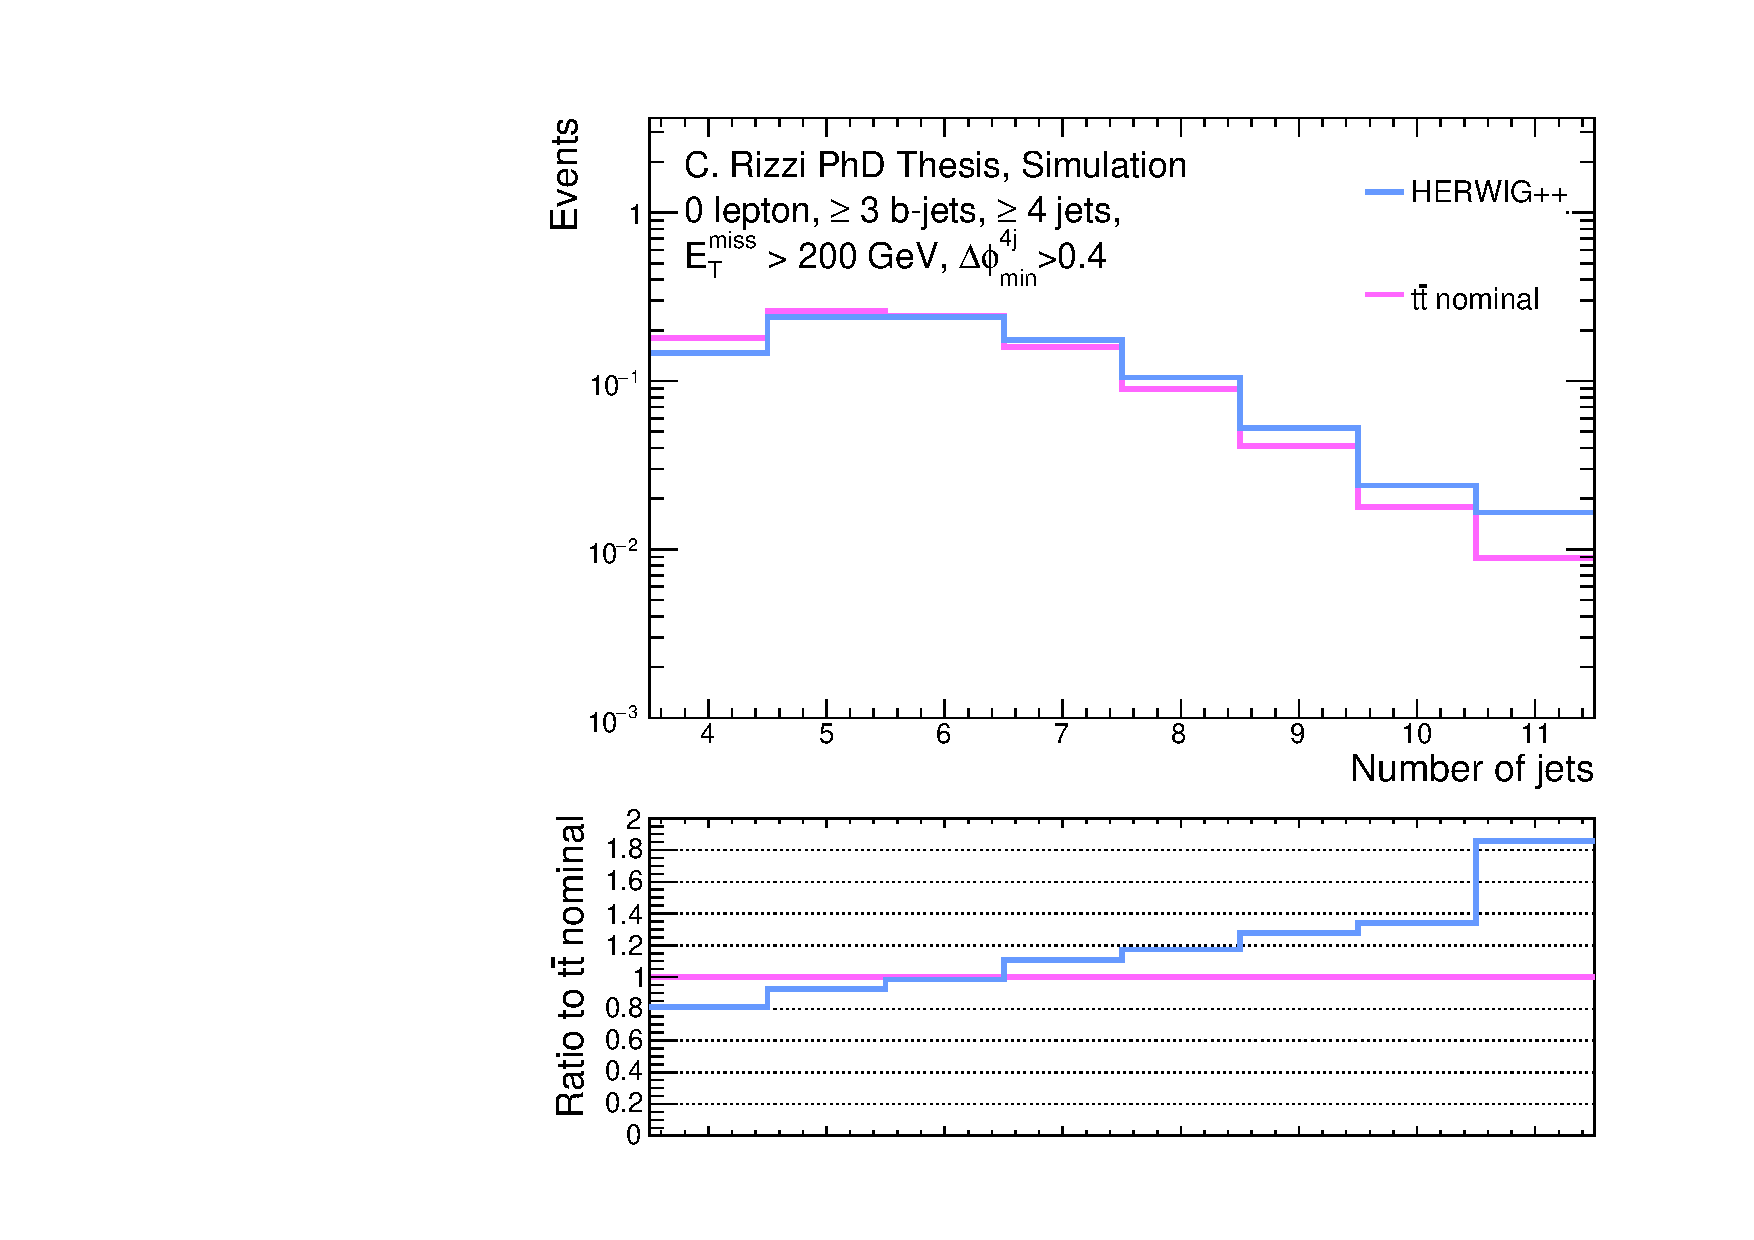
\includegraphics[width=0.32\textwidth]{figures/susy_common/ttbar_syst_ps/0L_3b/compare_jets_n_ttbar_syst_3b_scale.pdf}\label{fig:ttbar_nj_0L_ps}}
\subfigure[]{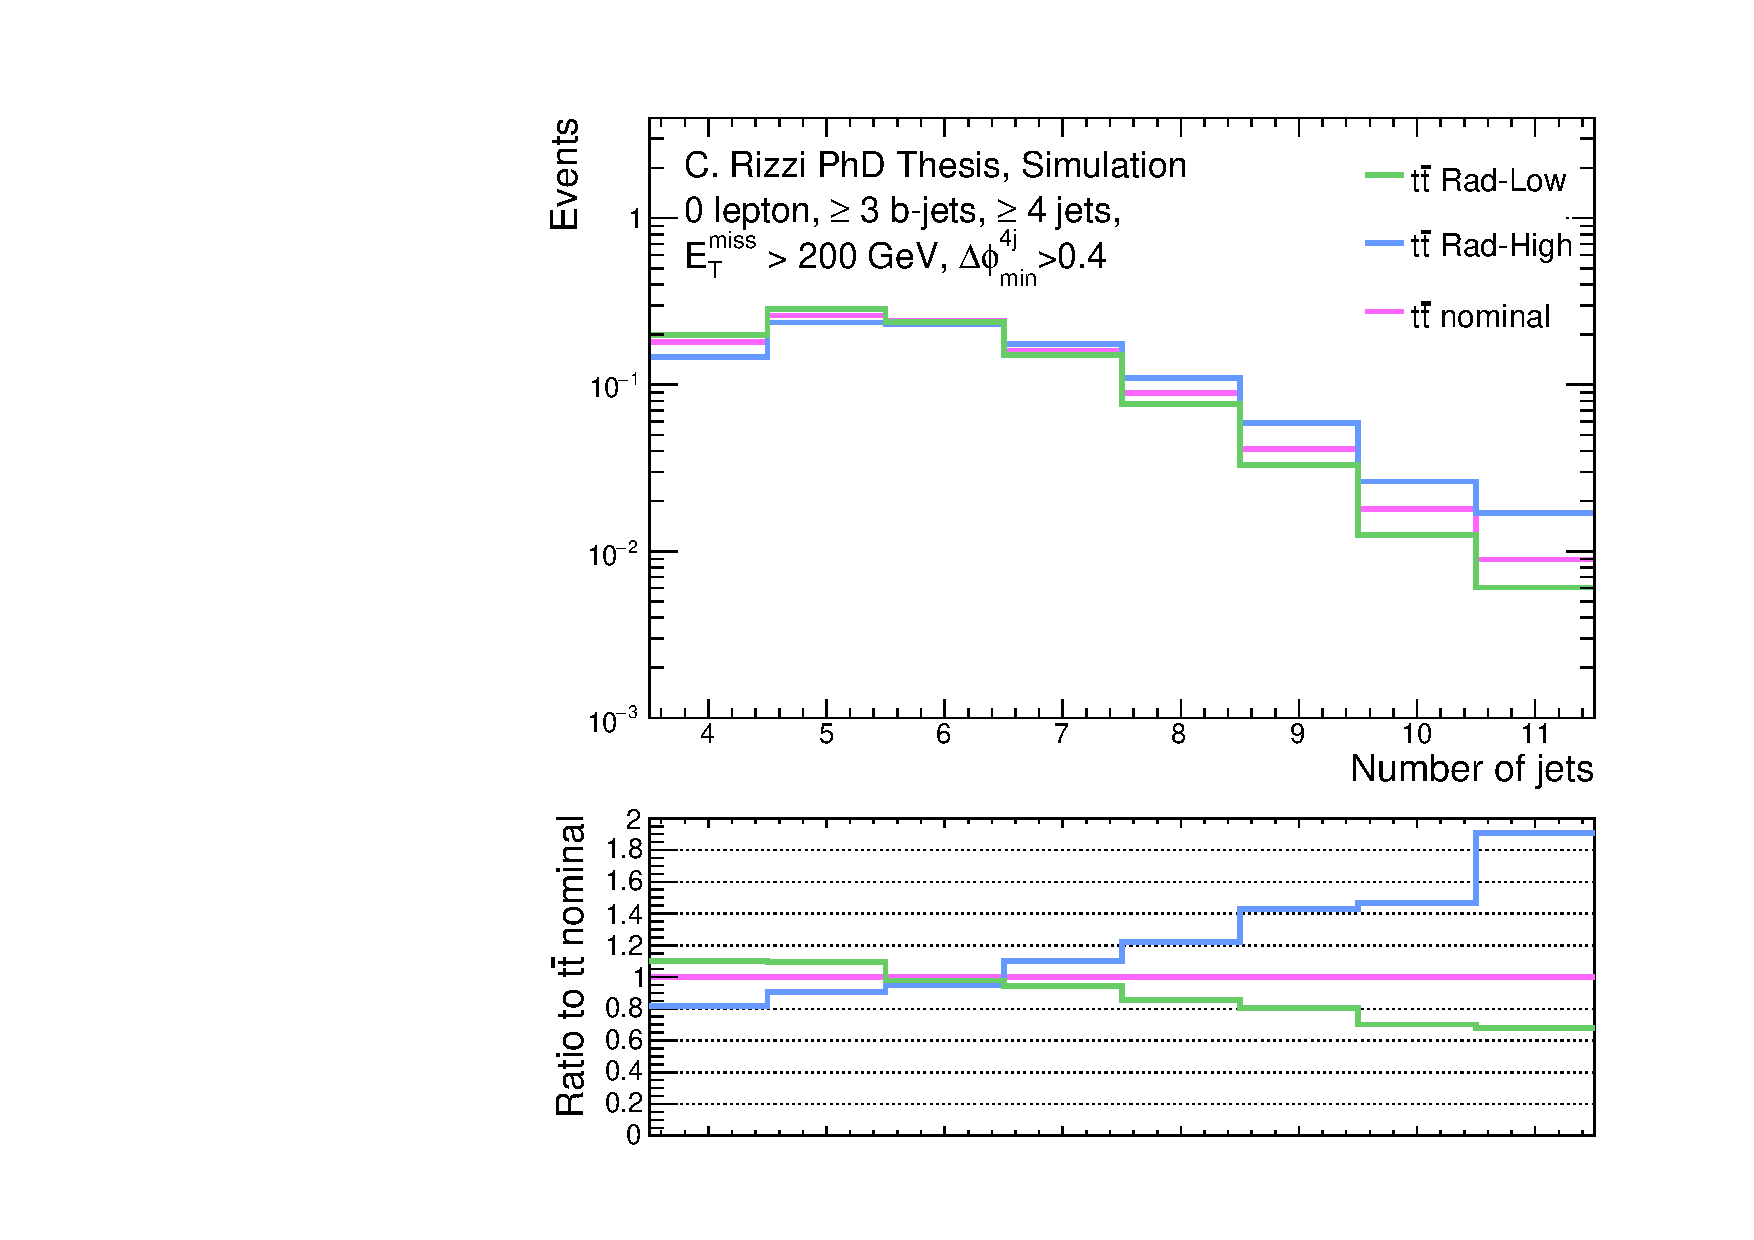
\includegraphics[width=0.32\textwidth]{figures/susy_common/ttbar_syst_rad/0L_3b/compare_jets_n_ttbar_syst_3b_scale.pdf}\label{fig:ttbar_nj_0L_rad}}
\caption{Distribution normalized to unity of the number of signal jets in the \ttbar \gls{mc} sample in a selection requiring at least four jets, at least two $b$-jets, $\met>200$ GeV and exactly zero lepton. 
\subref{fig:ttbar_nj_0L_gen} \PowhegBox (pink line) and \aNLO (blue line), both interfaced with \HWpp.
\subref{fig:ttbar_nj_0L_ps} Nominal sample (pink line), generated with \PowhegBox and showered with \PY, and a sample generated with \PowhegBox and showered with \HWpp (blue line).
\subref{fig:ttbar_nj_0L_rad} Nominal sample (pink line) and two varied samples generated with \PowhegBox interfaced with two versions of \PY (blue and green line).
%Distribution normalized to unity of the number of signal jets in the \ttbar \gls{mc} sample in a selection requiring at least four jets, at least two $b$-jets, $\met>200$ GeV and exactly zero lepton. 
%\subref{fig:ttbar_nj_0L_gen} Comparison of \PowhegBox (pink line) with \aNLO (blue line), both interfaced with \HWpp.
%\subref{fig:ttbar_nj_0L_ps} Comparison of the nominal sample (pink line), generated with \PowhegBox and showered with \PY, with a sample generated with \PowhegBox and showered with \HWpp (blue line).
%\subref{fig:ttbar_nj_0L_rad} Comparison of the nominal sample (pink line) with two varied samples generated with \PowhegBox interfaced with two versions of \PY (blue and green line).
}\label{fig:ttbar_nj_0L_syst}
\end{figure}

\begin{figure}[htb]
\centering 
\subfigure[]{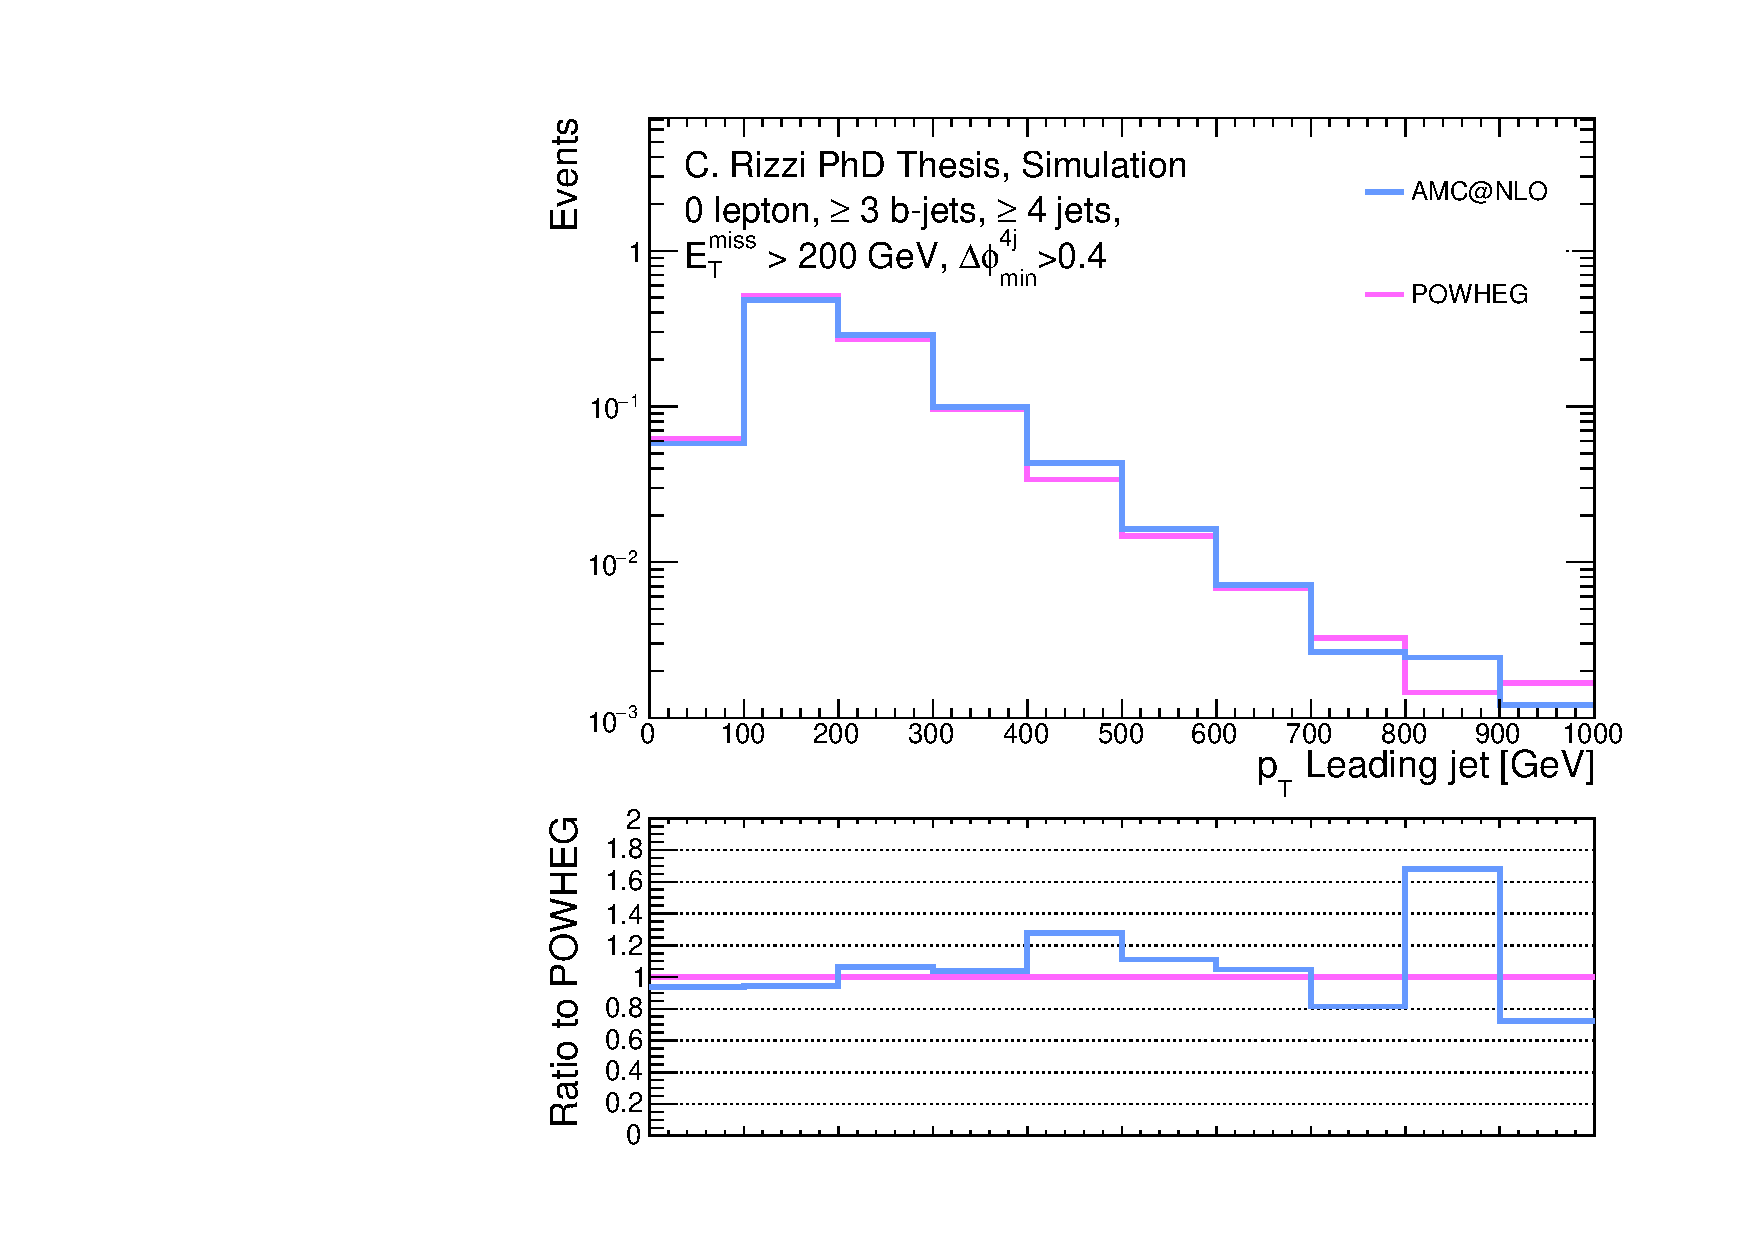
\includegraphics[width=0.32\textwidth]{figures/susy_common/ttbar_syst_gen/0L_3b/compare_pt_jet_1_ttbar_syst_3b_scale.pdf}\label{fig:ttbar_ptj1_0L_gen}}
\subfigure[]{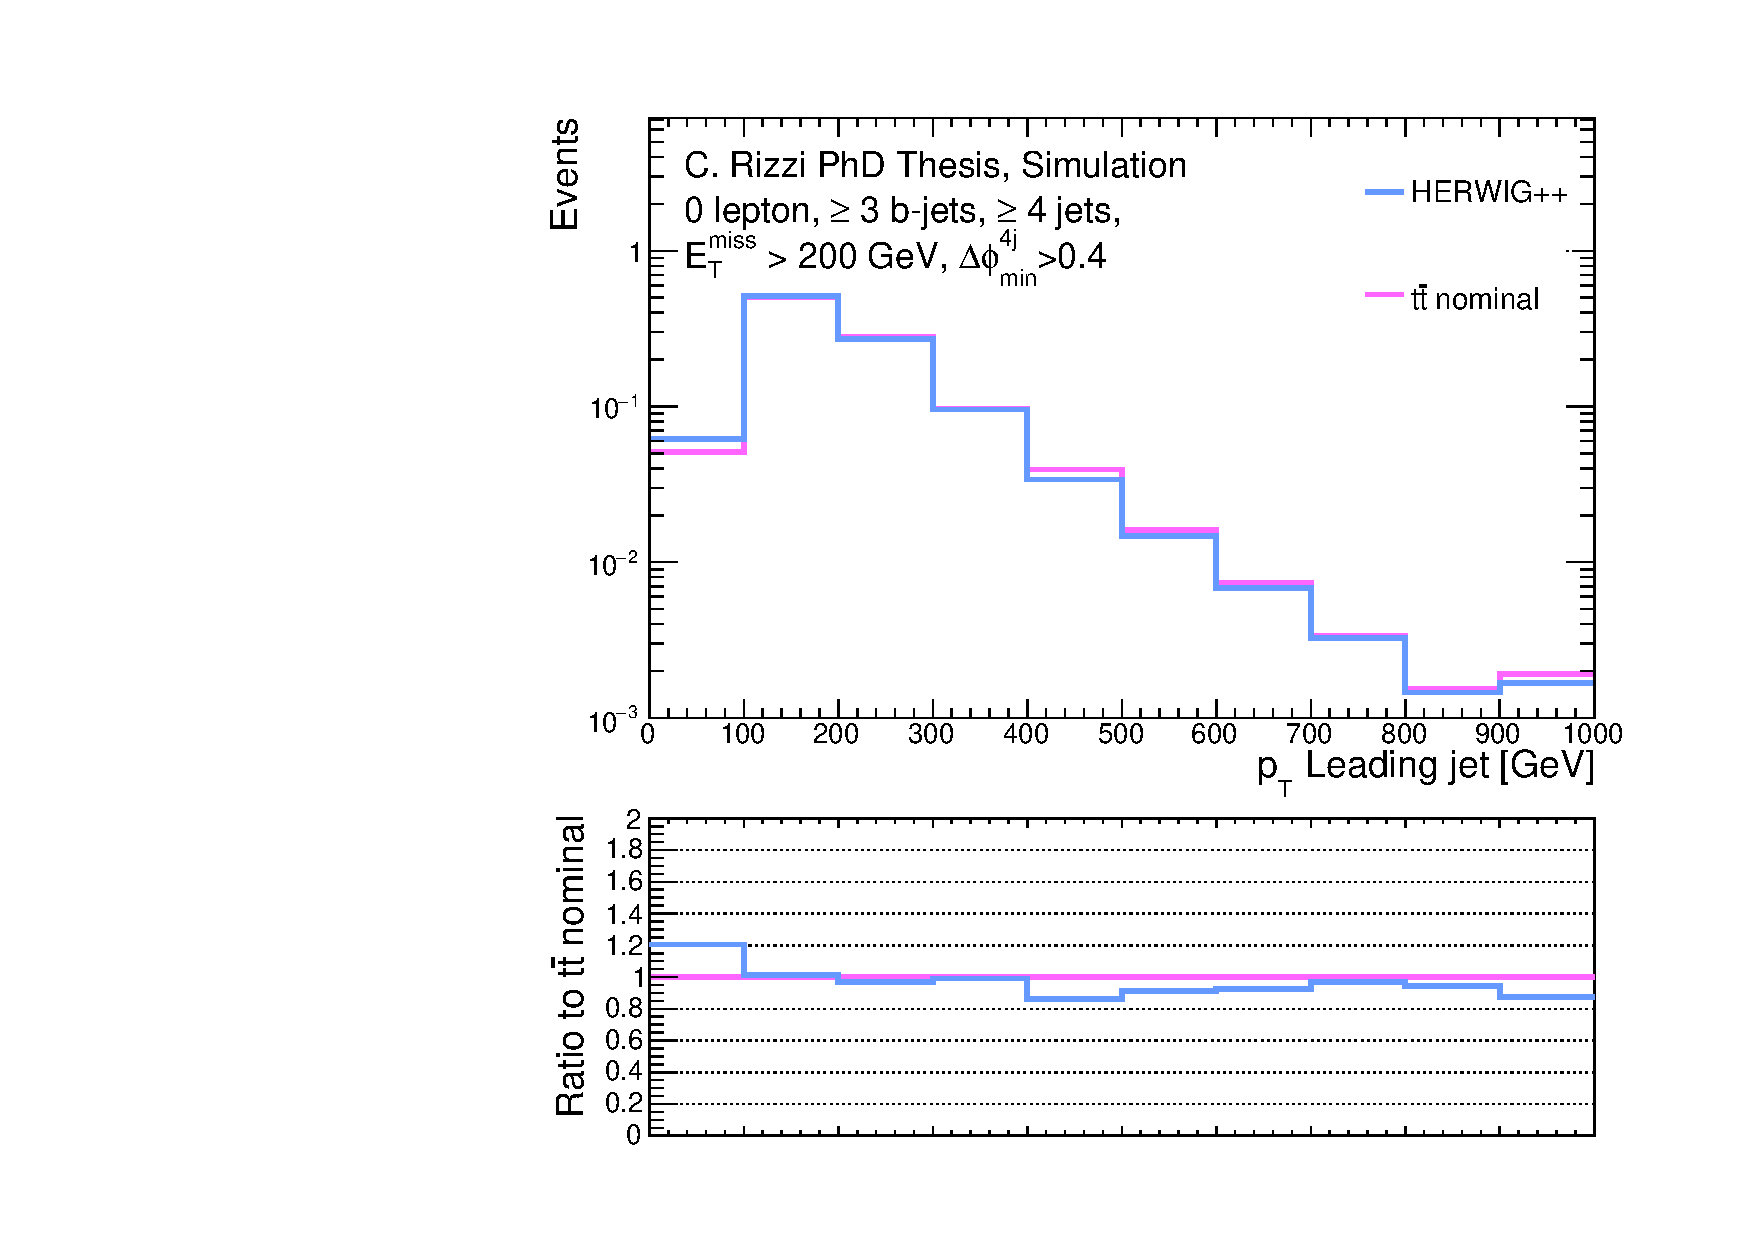
\includegraphics[width=0.32\textwidth]{figures/susy_common/ttbar_syst_ps/0L_3b/compare_pt_jet_1_ttbar_syst_3b_scale.pdf}\label{fig:ttbar_ptj1_0L_ps}}
\subfigure[]{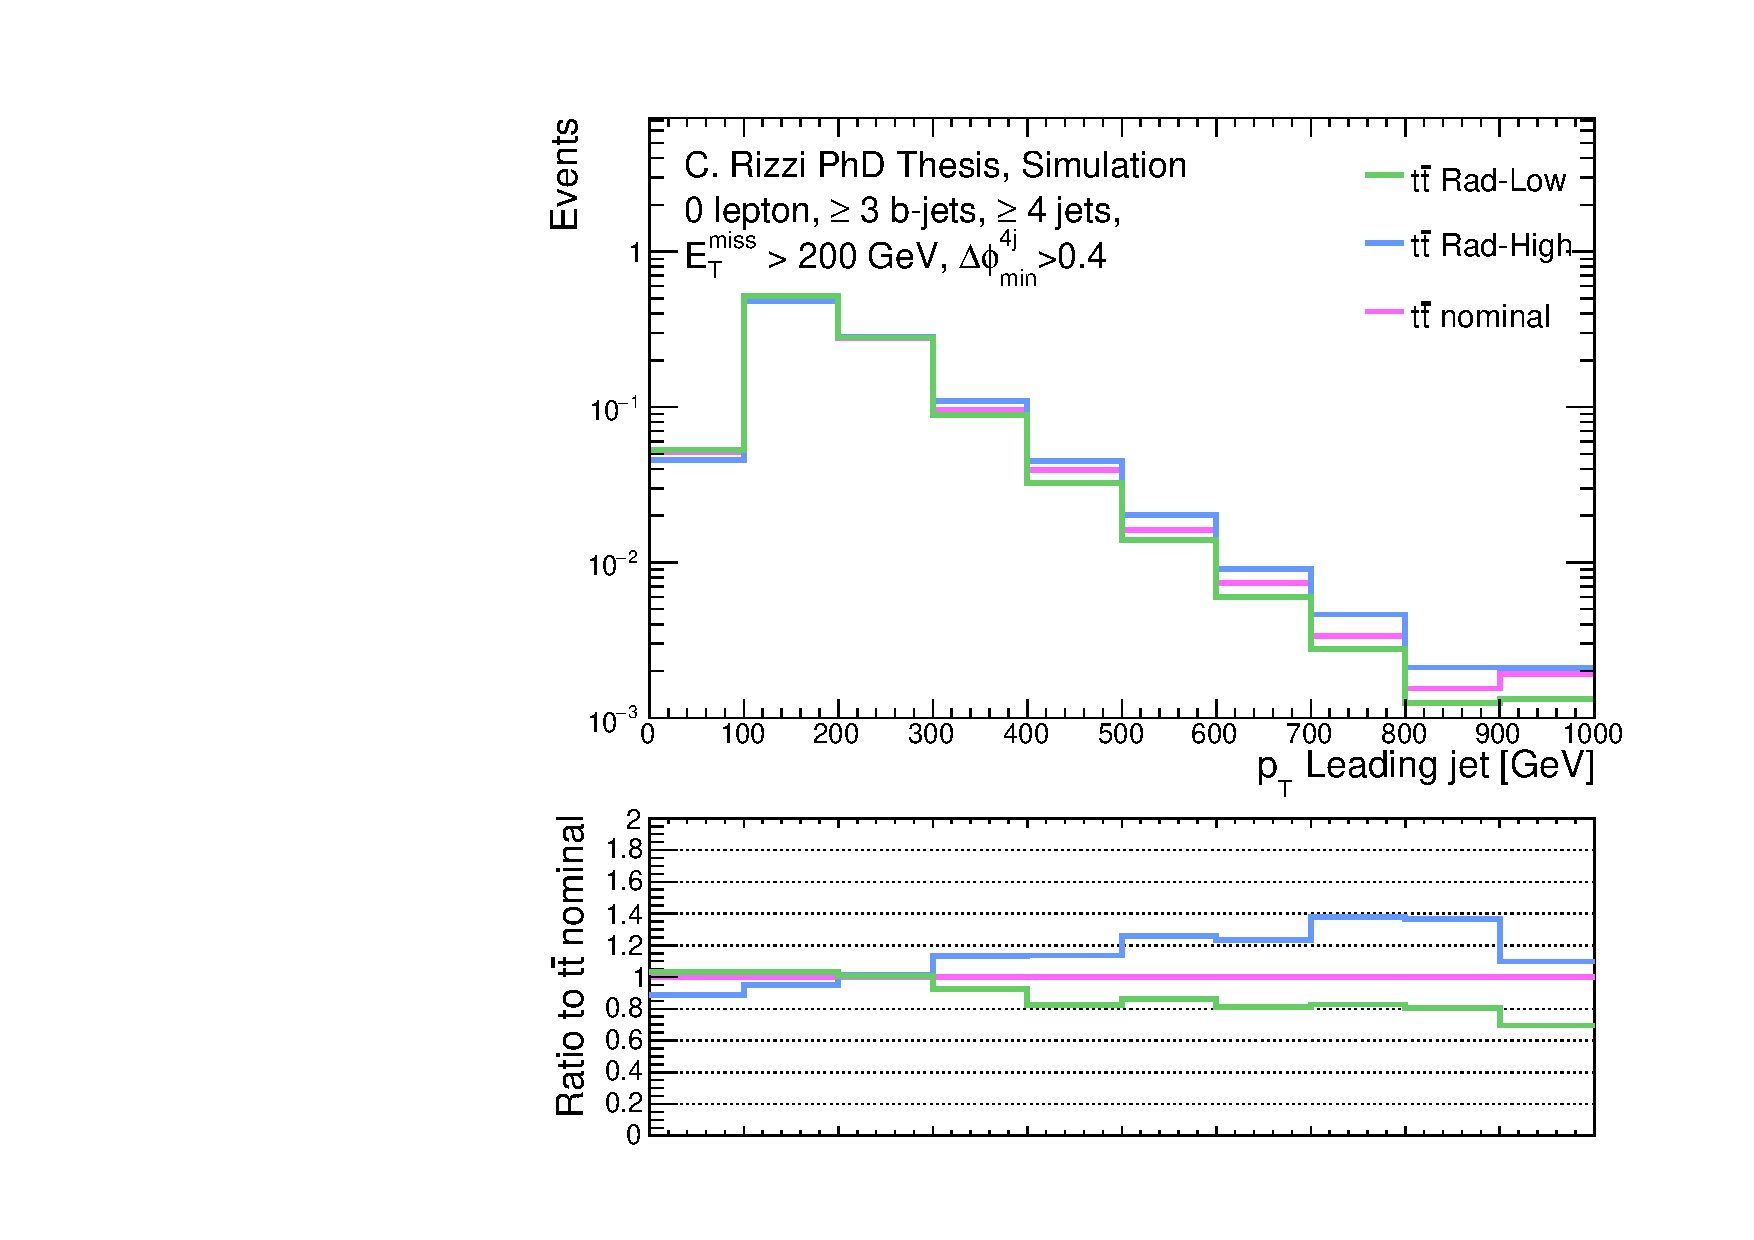
\includegraphics[width=0.32\textwidth]{figures/susy_common/ttbar_syst_rad/0L_3b/compare_pt_jet_1_ttbar_syst_3b_scale.pdf}\label{fig:ttbar_ptj1_0L_rad}}
\caption{Distribution normalized to unity of the \pt of the leading signal jet in the \ttbar \gls{mc} sample in a selection requiring at least four jets, at least two $b$-jets, $\met>200$ GeV and exactly zero lepton. 
\subref{fig:ttbar_nj_0L_gen} \PowhegBox (pink line) and \aNLO (blue line), both interfaced with \HWpp.
\subref{fig:ttbar_nj_0L_ps} nominal sample (pink line), generated with \PowhegBox and showered with \PY, and a sample generated with \PowhegBox and showered with \HWpp (blue line).
\subref{fig:ttbar_nj_0L_rad} Nominal sample (pink line) and two varied samples generated with \PowhegBox interfaced with two versions of \PY (blue and green line).}\label{fig:ttbar_ptj1_0L_syst}
\end{figure}


The main limitation for the estimate of the uncertainties is the statistical uncertainty of the \gls{mc} samples for the systematic variations, as these samples have in general less simulated events than the nominal sample. 
More statistics is available at particle level, where the simulation of the interaction of the particles with the detector and the following event reconstruction (discussed in Section \ref{sec:detsim}) is not performed, so the evaluation of the \ttbar modelling uncertainties is carried out 
comparing samples at particle level, with the assumption that the detector simulation has a similar effect on all the samples, 
independently of the \gls{mc} generator used. Two further strategies are in place to allow enough statistics in the comparison of the different samples. 
One consists in relaxing or removing some selections to both the \glspl{cr} and the corresponding \glspl{sr}/\glspl{vr}. 
Another is to substitute the selection on the number of $b$-jets with truth-tagging, described in the next section.

\subsubsection*{Truth $b$-tagging}

With truth tagging, instead of keeping only the events that satisfy a certain criterion on the number of $b$-tagged jets, all the events are kept and weighted. The weight is the probability that, out of all selected jets in the event,
a certain number pass the $b$-tagging identification.
A different weight is computed for each $b$-tagging requirement; 
for example, the probability for the event to have at least three $b$-tagged jets will be different from the probability of having exactly two. 
For each jet, the probability to be $b$-tagged can be expressed as a function of the jet flavor ($f$), \pt and $\eta$:

\begin{equation}
\varepsilon \left(f,|\eta|,p_{\mathrm{T}}\right) \; .
\label{eq:susy_common:btageff}
\end{equation}

\noindent If an event has $N$ jets, the probability of containing exactly one $b$-tag jet can be expressed as:
\begin{equation}
        P_{=1} = \sum\limits_{i=1}^N \left( \varepsilon_{i} \prod\limits_{i \neq j} \left( 1 - \varepsilon_{j} \right) \right) \; ,
\end{equation}

\noindent and in the same way, we can compute the probability for an inclusive $b$-tagging selection:
\begin{equation}
 \begin{split}
        P_{=0} &= \prod\limits_{i=1}^N \left( 1 - \varepsilon_{j} \right) \; ,\\
        P_{\geq 1} &= 1 - P_{=0} \; .
 \end{split}
\end{equation} 
 
\noindent This procedure can be extended to an arbitrary number of $b$-tagged jets by summing over all the possible permutations that lead to the desired number of $b$-tagged jets ($n$) to derive the exclusive probability and then subtract it from the $P_{\geq n}$ probability to have the inclusive probability for $\geq n+1$ $b$-tagged jets.
 
Beside decreasing the statistical uncertainty on the expected number of events, the other advantage of using truth tagging on particle-level samples is that it allows to emulate the reconstruction-level efficiency of the $b$-tagging algorithm: 
at particle-level a jet is considered a $b$-tagged if it is matched to a $b$-quark in the \gls{mc} record within a certain cone. This criterion has 
almost 100\% efficiency for real $b$-jets, and it leads to a null mistag rate. Instead with truth tagging, if the efficiency map used in Equation \ref{eq:susy_common:btageff} corresponds to the $b$-tagging efficiency measured for reconstructed jets, 
it is possible to obtain the same efficiency to a $b$-tagging selection as in a reconstructed-level analysis. 

Some analysis variables are build using explicitly the kinematic characteristics of the $b$-tagged jets, e.g. \mtb. The truth tagging method allows to choose which jets in the event should be considered as $b$-tagged: in an event with $N$ jets, each permutation with a $n$ jets considered as $b$-tagged and $N-n$ jets considered as non $b$-tagged is characterized by an individual weight $w_i$. If we define $S$ the sum of all these individual weights, a pseudo-random number generated with uniform probability between 0 and $S$ will indicate which permutation to choose and consequently which jets to consider as $b$-tagged; this procedure is illustrated in Figure \ref{fig:susy_common_trf_perm}. 

\begin{figure}[h]
\centering 
%\subfigure[]{
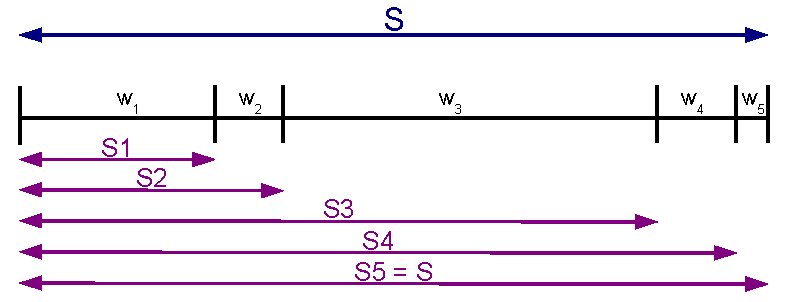
\includegraphics[width=0.6\textwidth]{figures/susy_common/trf_perm}
%}
\caption{Example schema to choose the selected permutation with truth $b$-tagging.}\label{fig:susy_common_trf_perm}
\end{figure}


\subsection{Single top quark production}

While the production of a \ttbar pair is mediated by the strong interaction, in the case of a single top quark the production occurs via the electroweak interaction. 
There are three possible production channels, illustrated in Fig. \ref{fig:single_top_prod}: the t-channel, the Wt-channel, where a top quark and a $W$ boson are produced, and the s-channel. 
The Wt- and s-channel production mechanisms are simulated with the same generator choice as \ttbar: \PowhegBox v2, showered with \PY v6.428.
Single top events produced through the t-channel process are simulated with \PowhegBox v1, which uses the four-flavor scheme for the computation of the \gls{nlo} \gls{me} and the CT10f4 \gls{partdf} set, with the four-flavor scheme as well, and the top quarks are decayed with \MadSpin \cite{Artoisenet:2012st}.
The cross section used for normalization is computed at \gls{nlo}+\gls{nnll} order 
\cite{Kidonakis:2011wy,Kidonakis:2010ux,Kidonakis:2010tc}.

\begin{figure}[h]
\centering 
\subfigure[]{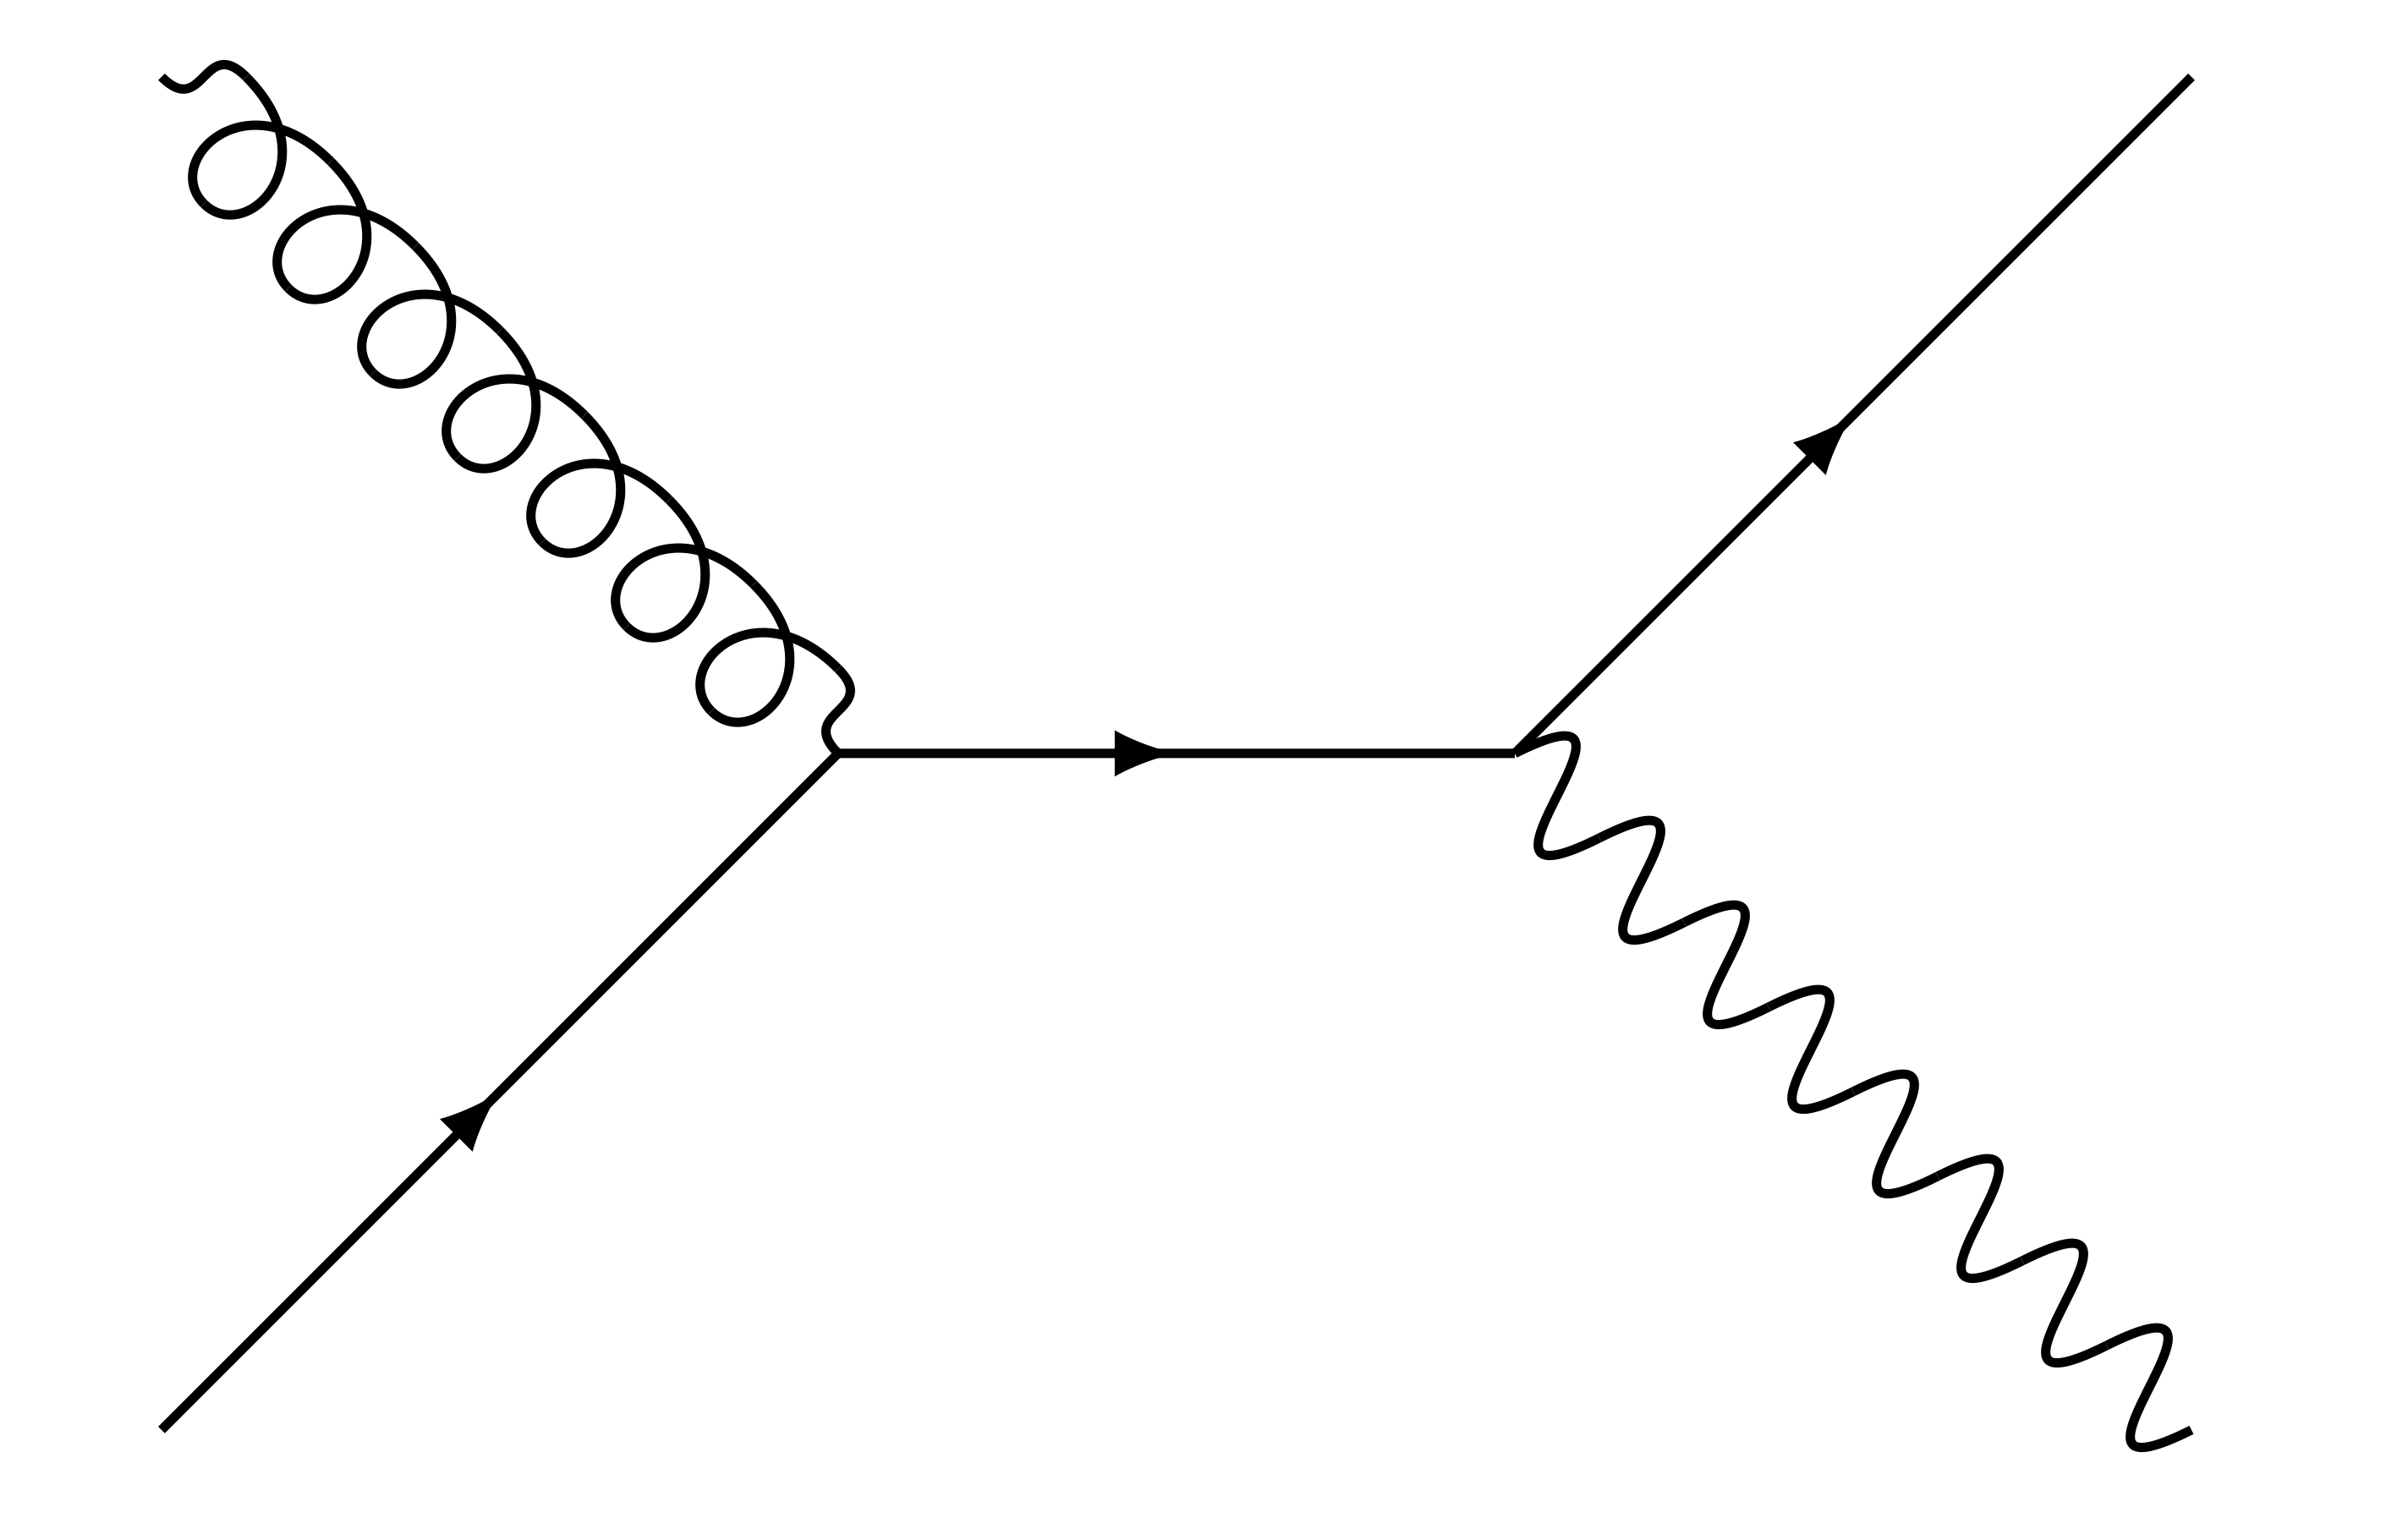
\includegraphics[width=0.3\textwidth]{figures/susy_common/feynman/st_2}\label{fig:st_prod_Wt1}}
\subfigure[]{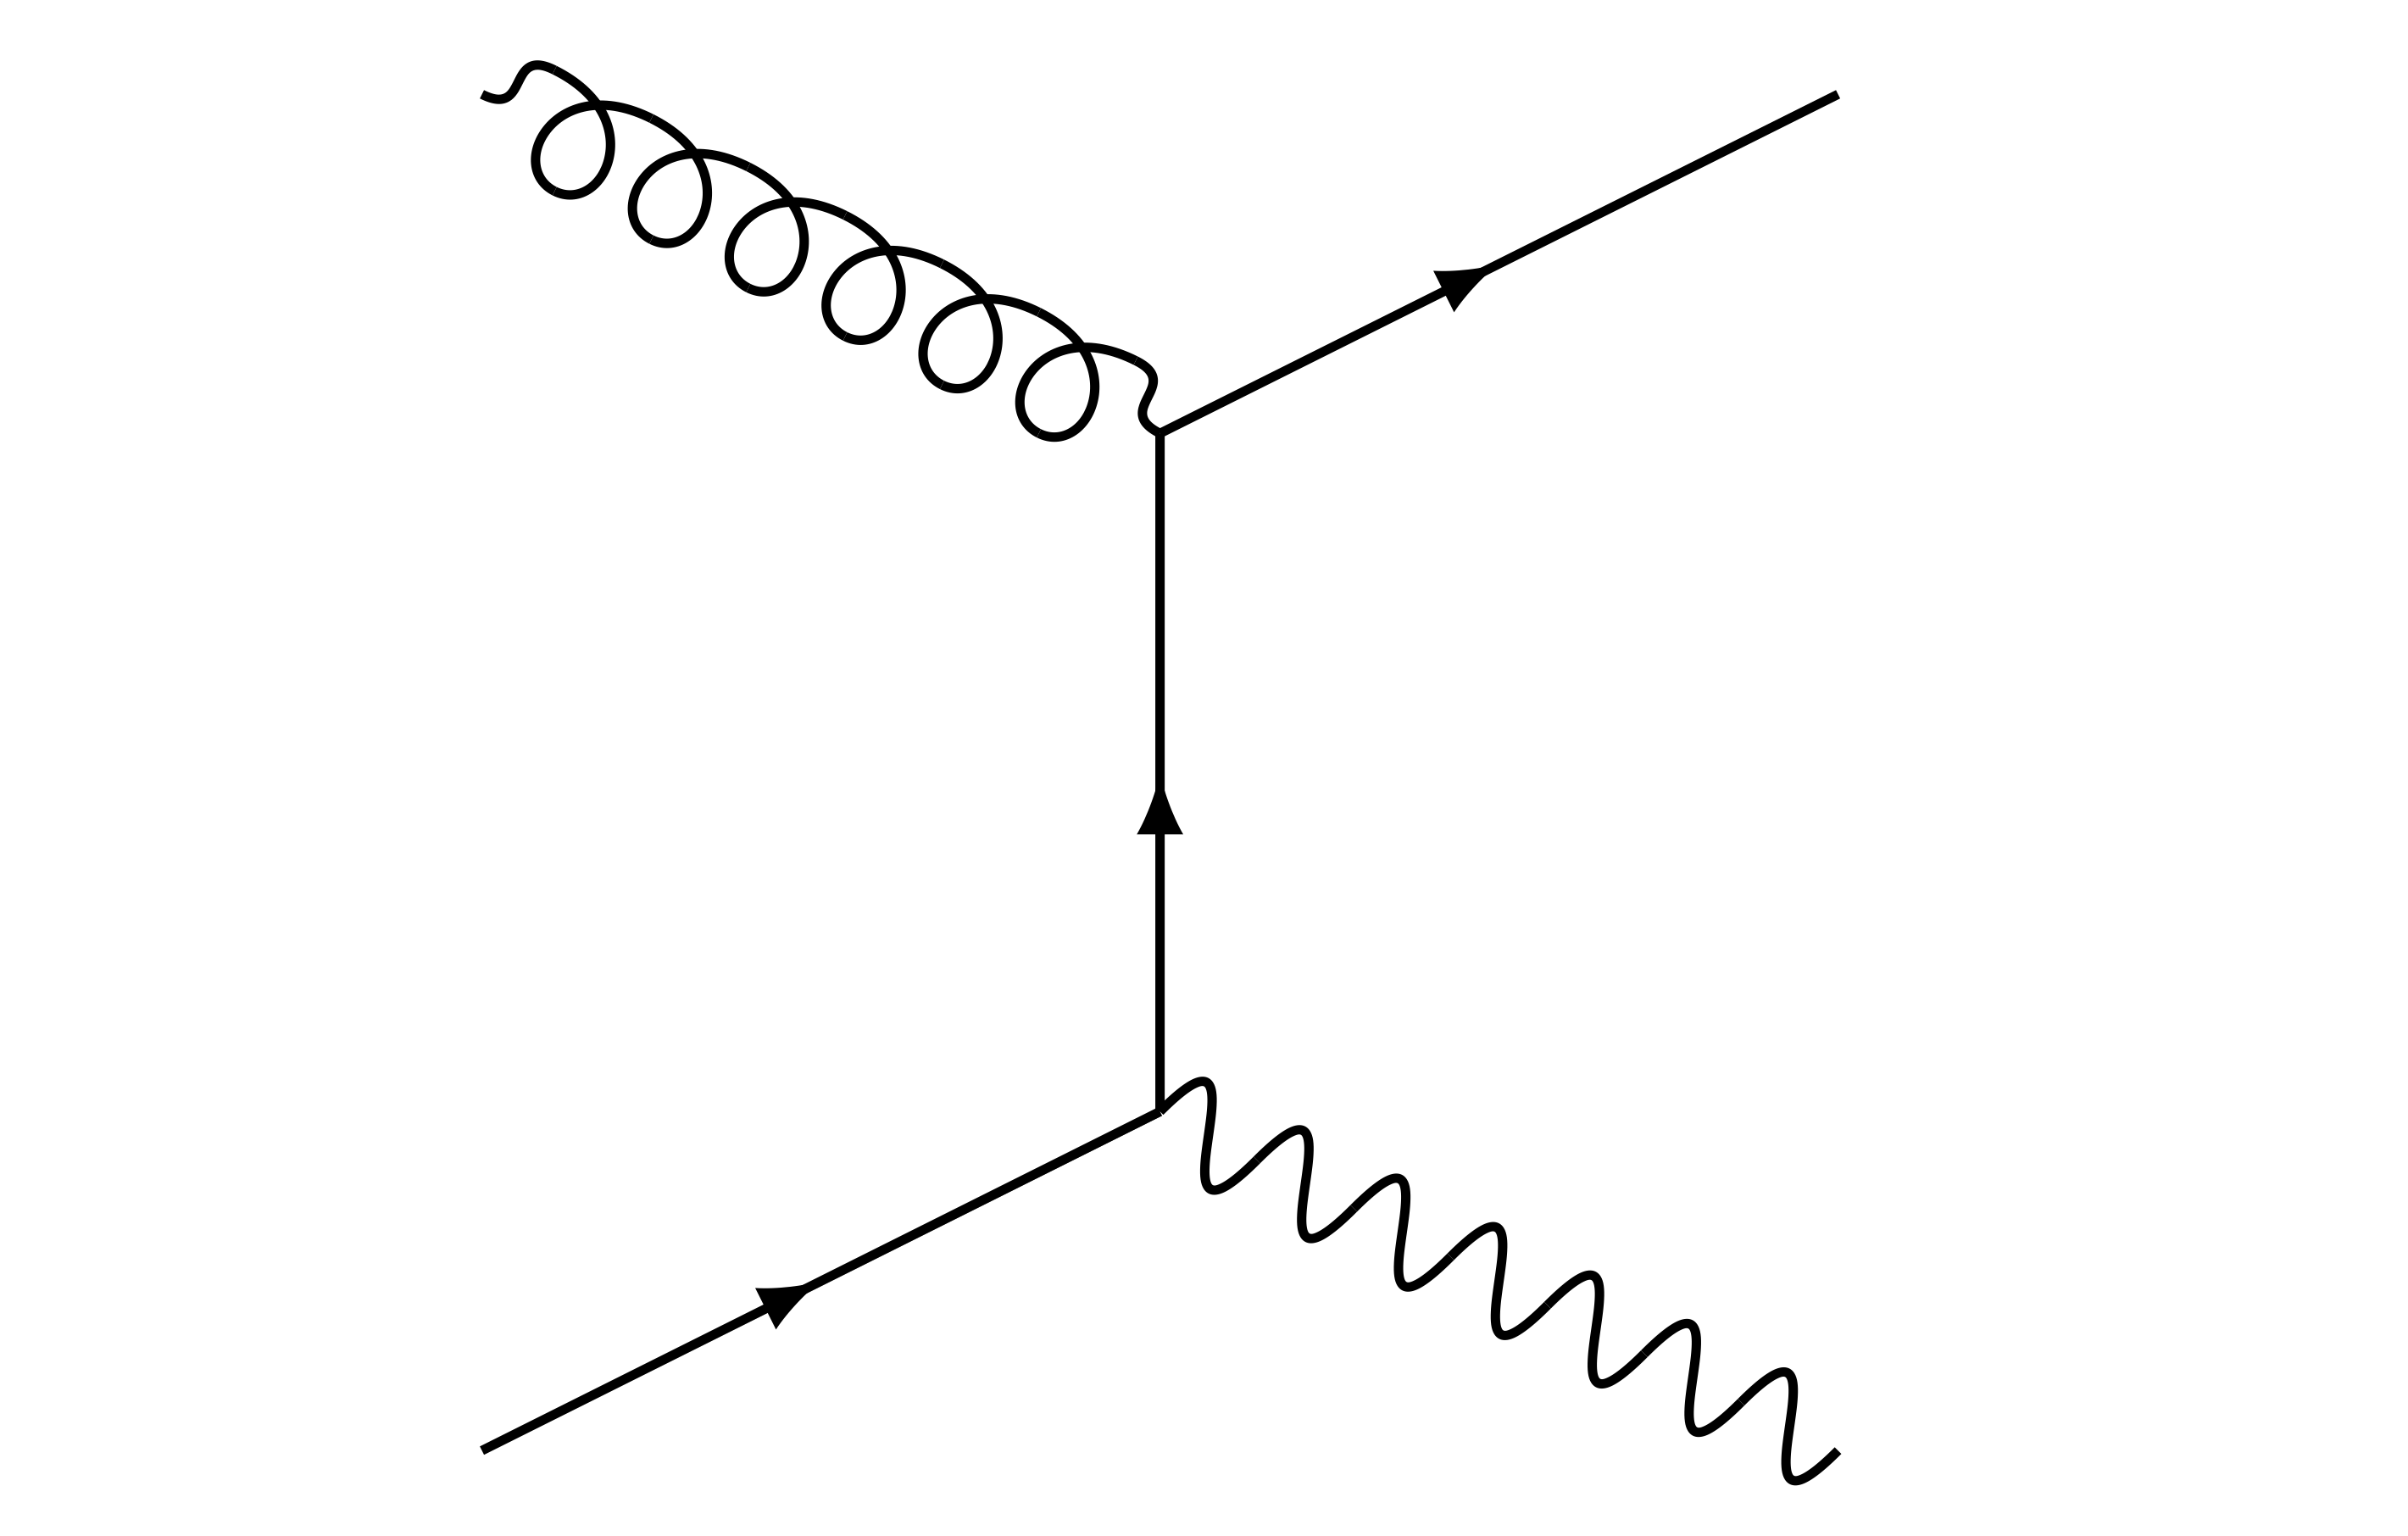
\includegraphics[width=0.3\textwidth]{figures/susy_common/feynman/st_3}\label{fig:st_prod_Wt2}} \\
\subfigure[]{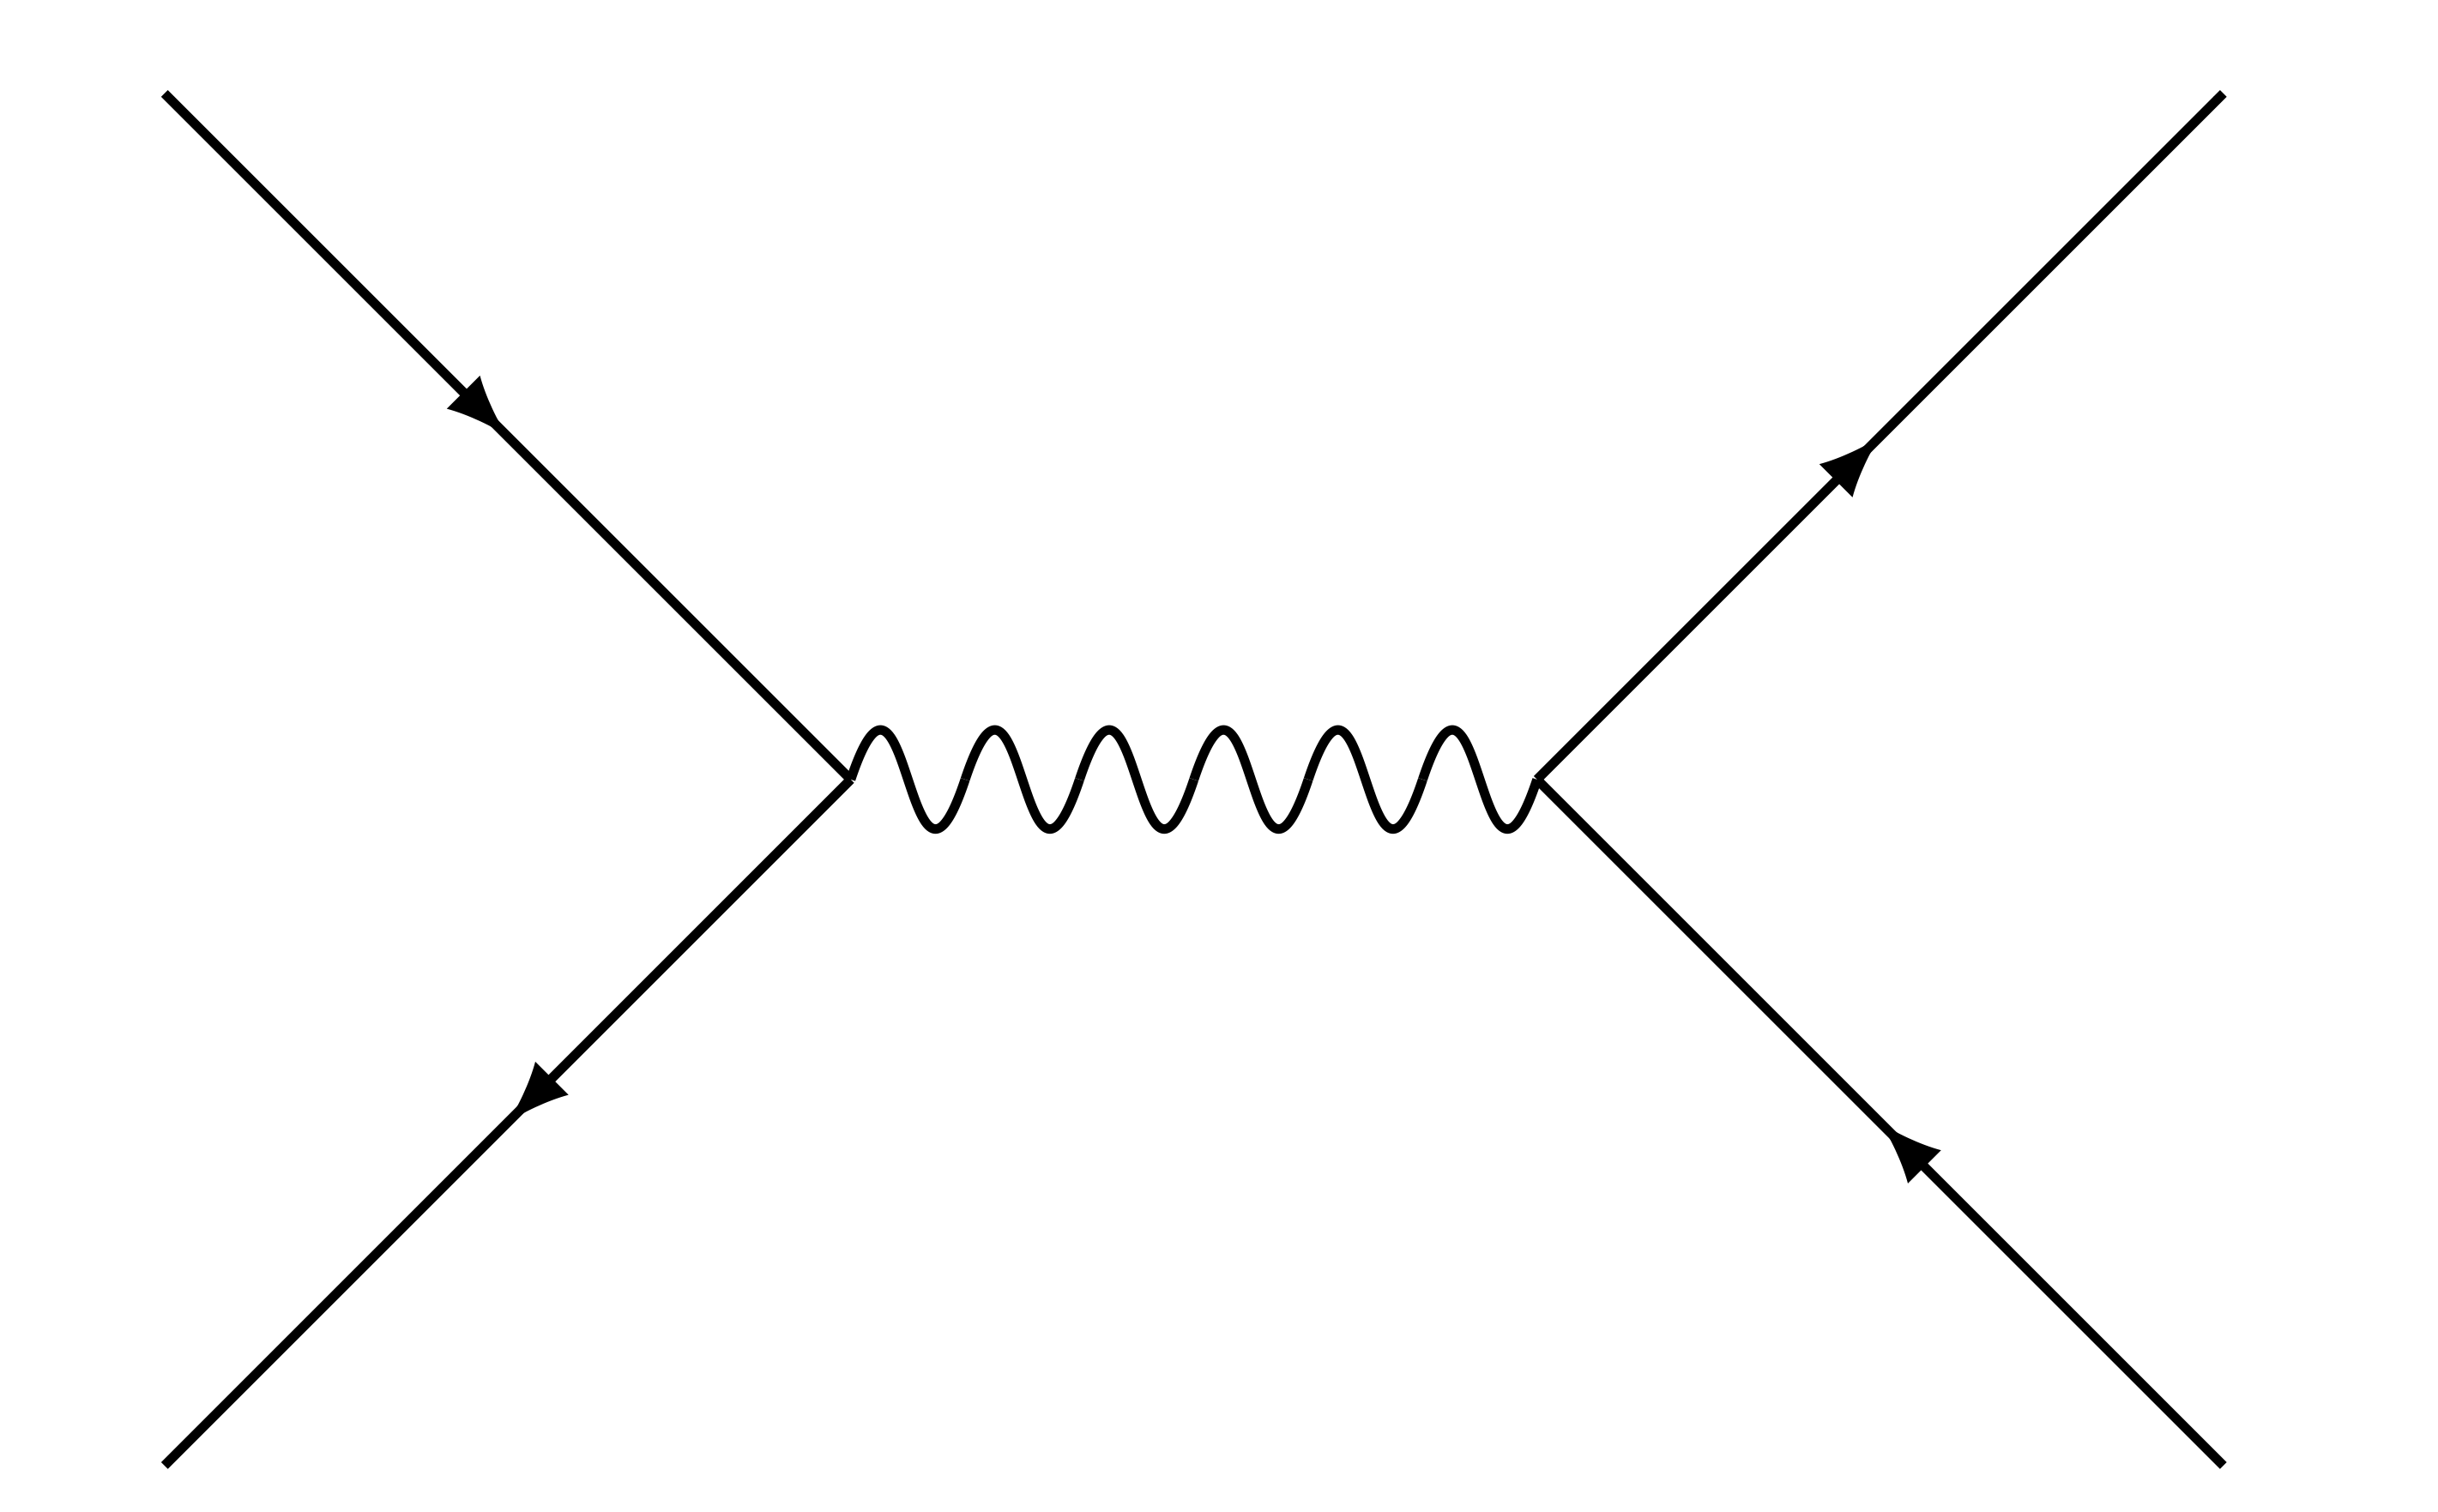
\includegraphics[width=0.3\textwidth]{figures/susy_common/feynman/st_4}\label{fig:st_prod_3}}
\subfigure[]{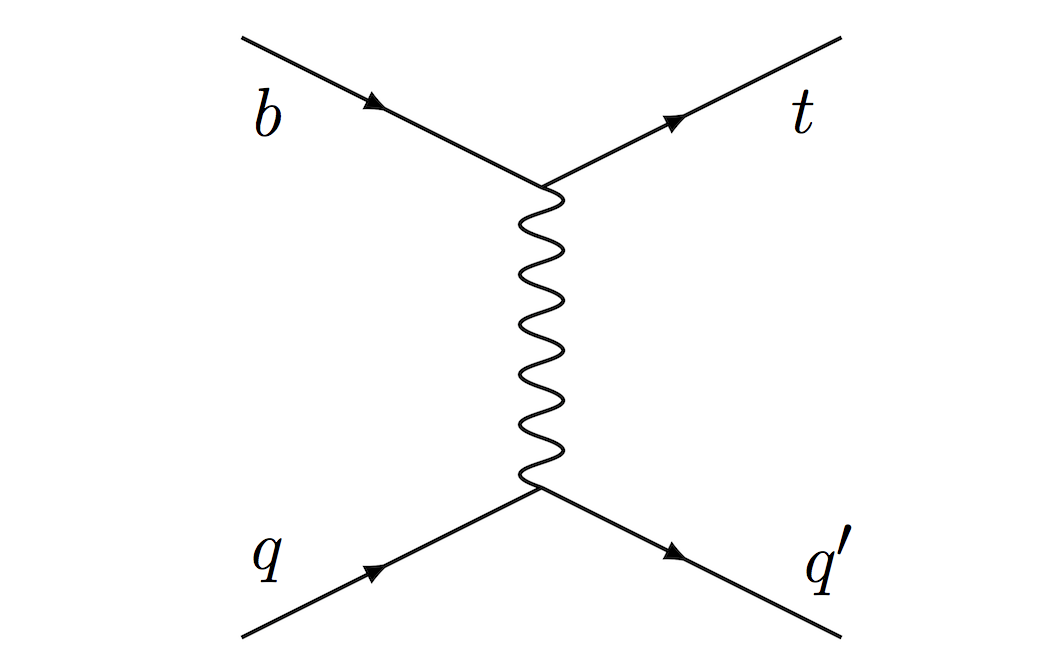
\includegraphics[width=0.3\textwidth]{figures/susy_common/feynman/st_5}\label{fig:st_prod_4}}
\caption{\Gls{lo} Feynman diagram for single top production. \subref{fig:st_prod_Wt1}-\subref{fig:st_prod_Wt2} Wt-channel. 
\subref{fig:st_prod_Wt2} s-channel. \subref{fig:st_prod_4} t-channel.}\label{fig:single_top_prod}
\end{figure}

\subsubsection*{Wt-channel and \ttbar interference}

While the \gls{lo} diagrams for Wt-channel single-top production in Figures \ref{fig:st_prod_Wt1} and \ref{fig:st_prod_Wt2} show a clear signature characterized by one single heavy-flavor quark in the final state,
when \gls{nlo} diagrams are considered it is possible to reach the same final state as with \ttbar production, namely $WWbb$, as shown in Fig. \ref{fig:WWbb_int}. 
Considering the two processes separately leads necessarily to an improper treatment of the quantum interference between them.
\PowhegBox allows to approach this problem with two different strategies, \gls{dr} and \gls{ds} \cite{Frixione:2005vw}; while none of them reproduces the quantum interference between single top and \ttbar, they allow to mitigate the size of the effect. 

\begin{figure}[h]
\centering 
\subfigure[]{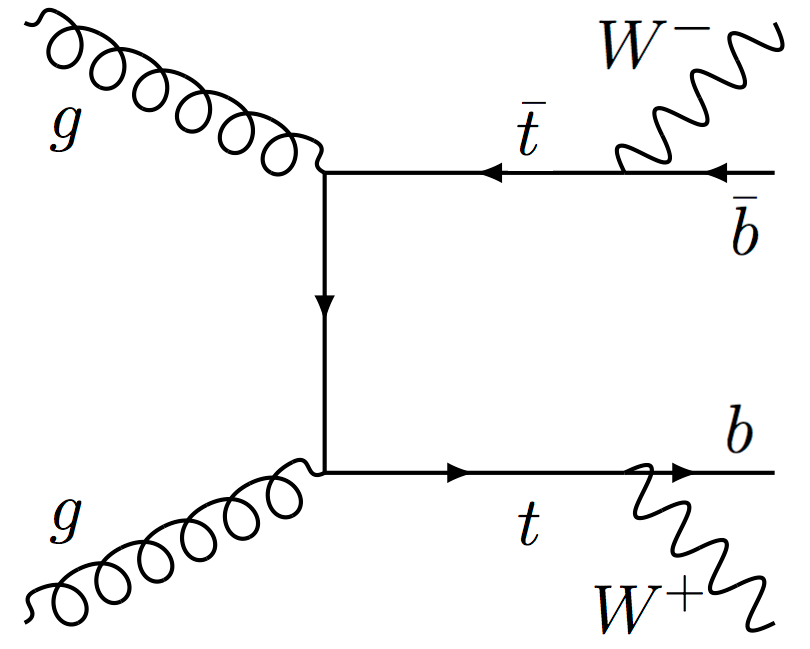
\includegraphics[width=0.25\textwidth]{figures/susy_common/feynman/ttbar_decay}\label{fig:ttbar_decay}}$\;\;\;\;\;\;$
\subfigure[]{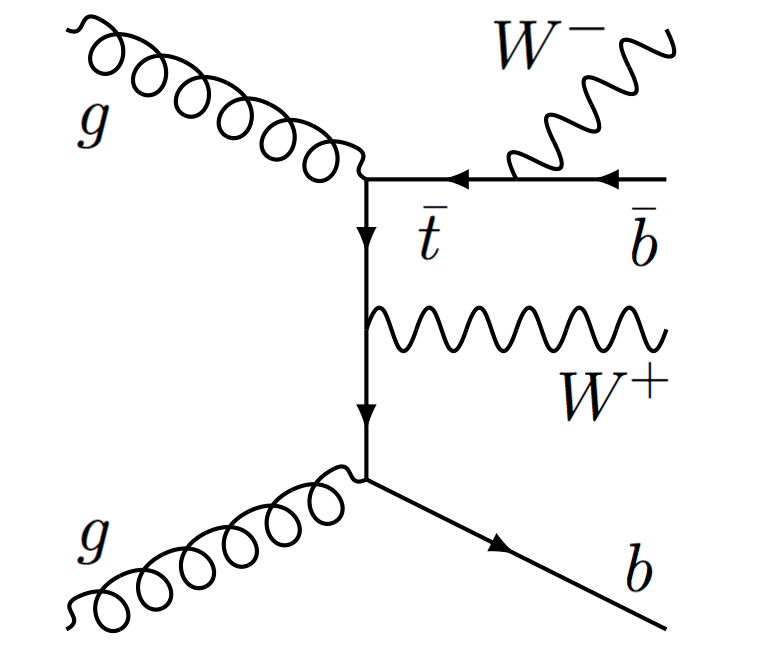
\includegraphics[width=0.25\textwidth]{figures/susy_common/feynman/Wt}\label{fig:Wt_nlo}} 
\caption{Two example diagrams that lead to a $WWbb$ final state. \subref{fig:ttbar_decay} double resonance, both $Wb$ pairs form a top quark. \subref{fig:Wt_nlo} single resonance, only one $Wb$ pair forms a top quark.}\label{fig:WWbb_int}
\end{figure}


We can write the matrix element for the production of the $WWbb$ final state as:

\begin{equation}
\mathcal{M}_{WWbb} = \mathcal{M}_{\rm{double-res}} + \mathcal{M}_{\rm{single-res}} \; ,
\end{equation}

\noindent where the first term represent the contribution from \ttbar production (double resonance) and the second term the contribution from 
\gls{nlo} corrections to the Wt single top production, where only one of the two $Wb$ systems is resonant (single resonance). 
When computing the squared amplitude, this becomes:

\begin{equation}
|\mathcal{M}_{WWbb}|^2 = |\mathcal{M}_{\rm{double-res}}|^2 + |\mathcal{M}_{\rm{single-res}}|^2 + 2 \mathcal{R}\left(\mathcal{M}_{\rm{double-res}}\times \mathcal{M}_{\rm{single-res}}^* \right) \; .
\end{equation}

While the first two terms are properly taken into account by the individual \ttbar and single top \gls{mc} simulations, 
the last term represent the interference between the two processes and, unless special care to avoid this is taken, it is completely ignored if the two processes are simulated independently. 

In the \gls{dr} approach, all the diagrams where a $W$ boson and a $b$-quark form a top quark are removed from the matrix element used to compute the single top cross-section in the Wt channel. While this approach is not gauge invariant, it is found to have negligible dependence on the gauge choice.

Instead in the \gls{ds} approach an extra subtraction term is added directly to the differential cross-section to cancel the contribution of the 
production of two on-shell top quarks, which is more accurate the more the invariant mass of the non-resonant $Wb$ system tends to the top quark mass. 
Acting at the cross-section level and not at the matrix-element level, this approach aims at accounting also for the interference term. 

Which one of the two strategies gives a better description of the data depends on the phase space under consideration. 
In this thesis the nominal single top estimate for the Wt channel is obtained with the \gls{dr} strategy. 
As an example, Figure \ref{fig:st_1L} shows how the choice of the \gls{dr} or \gls{ds} approach can change the distribution of two key variables 
in the analyses, \met and \mtb. 

\begin{figure}[h!]
\centering 
\subfigure[]{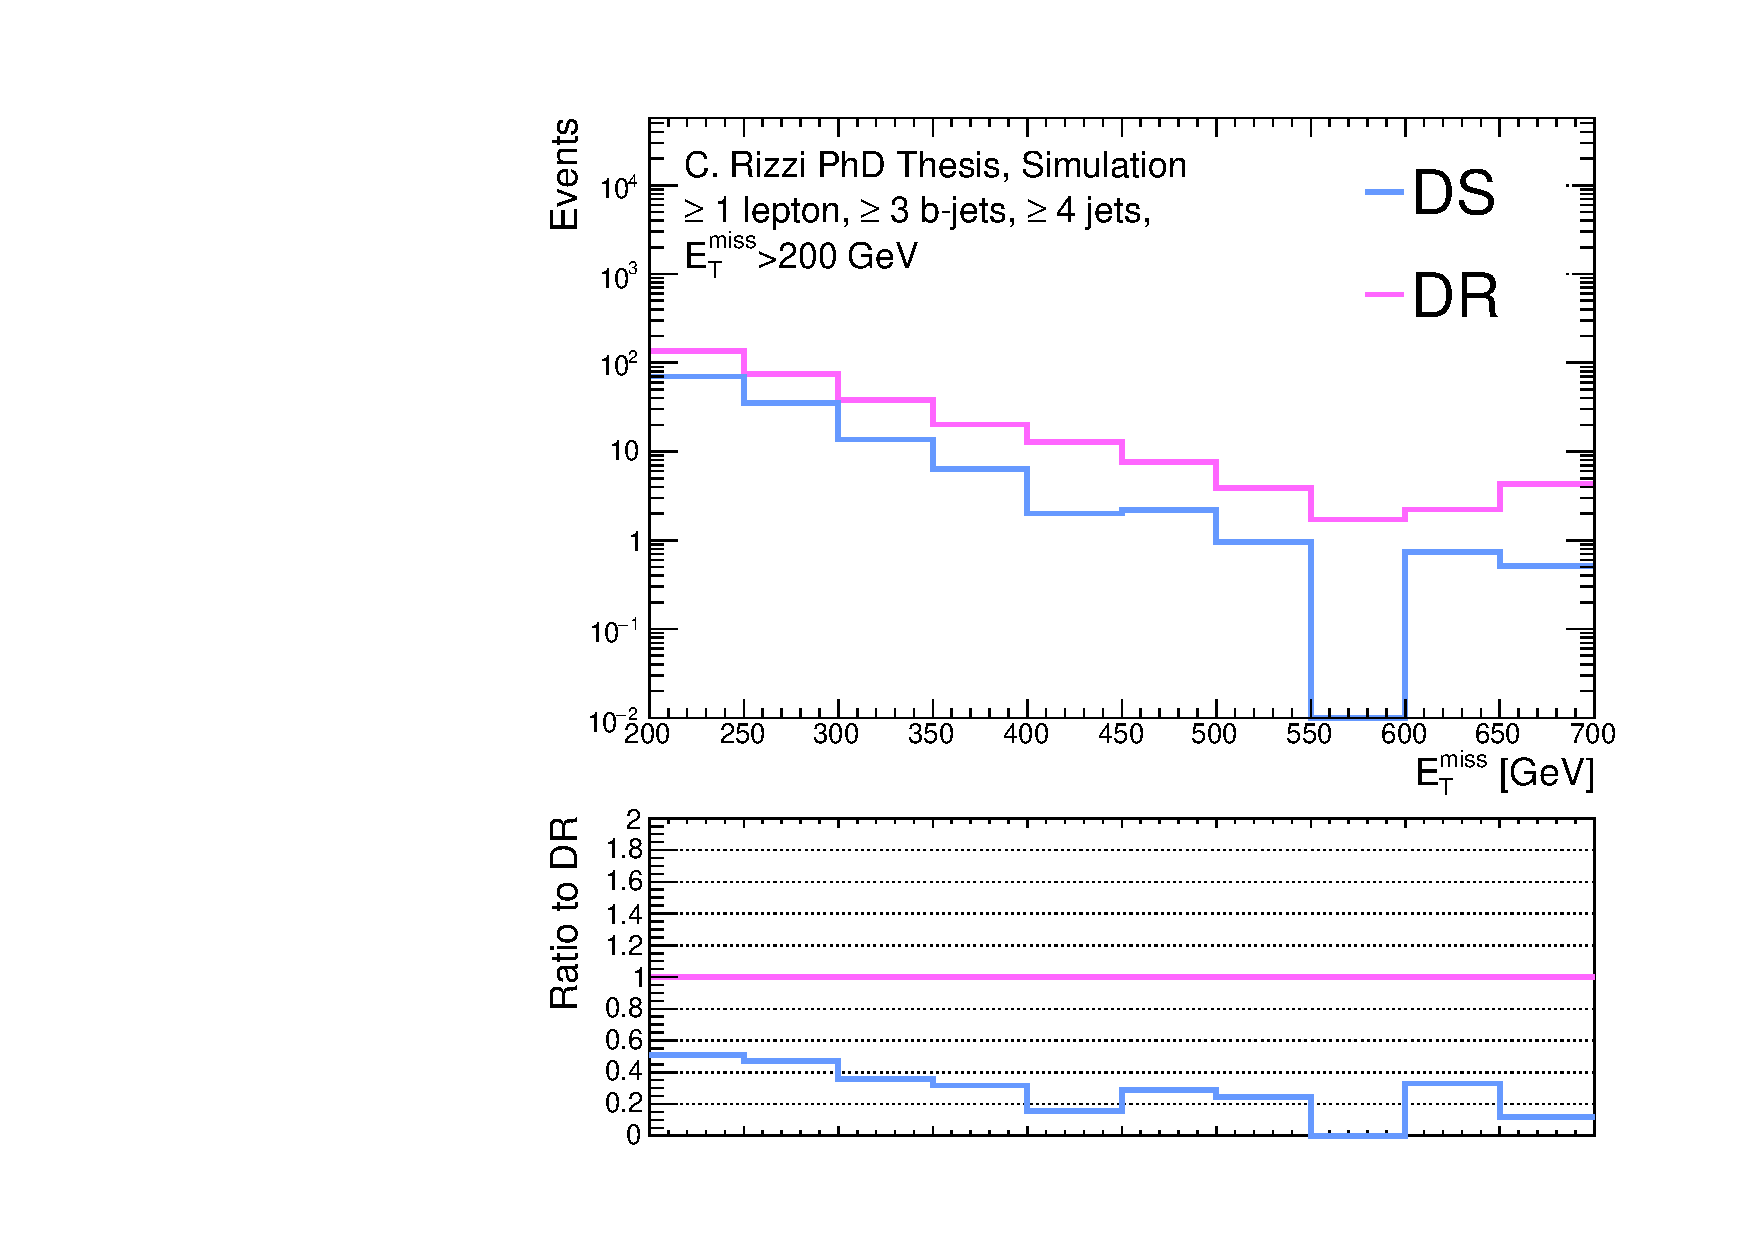
\includegraphics[width=0.32\textwidth]{figures/susy_common/st_DRDS/1L_3b/compare_met.pdf}\label{fig:st_met_1L}}
\subfigure[]{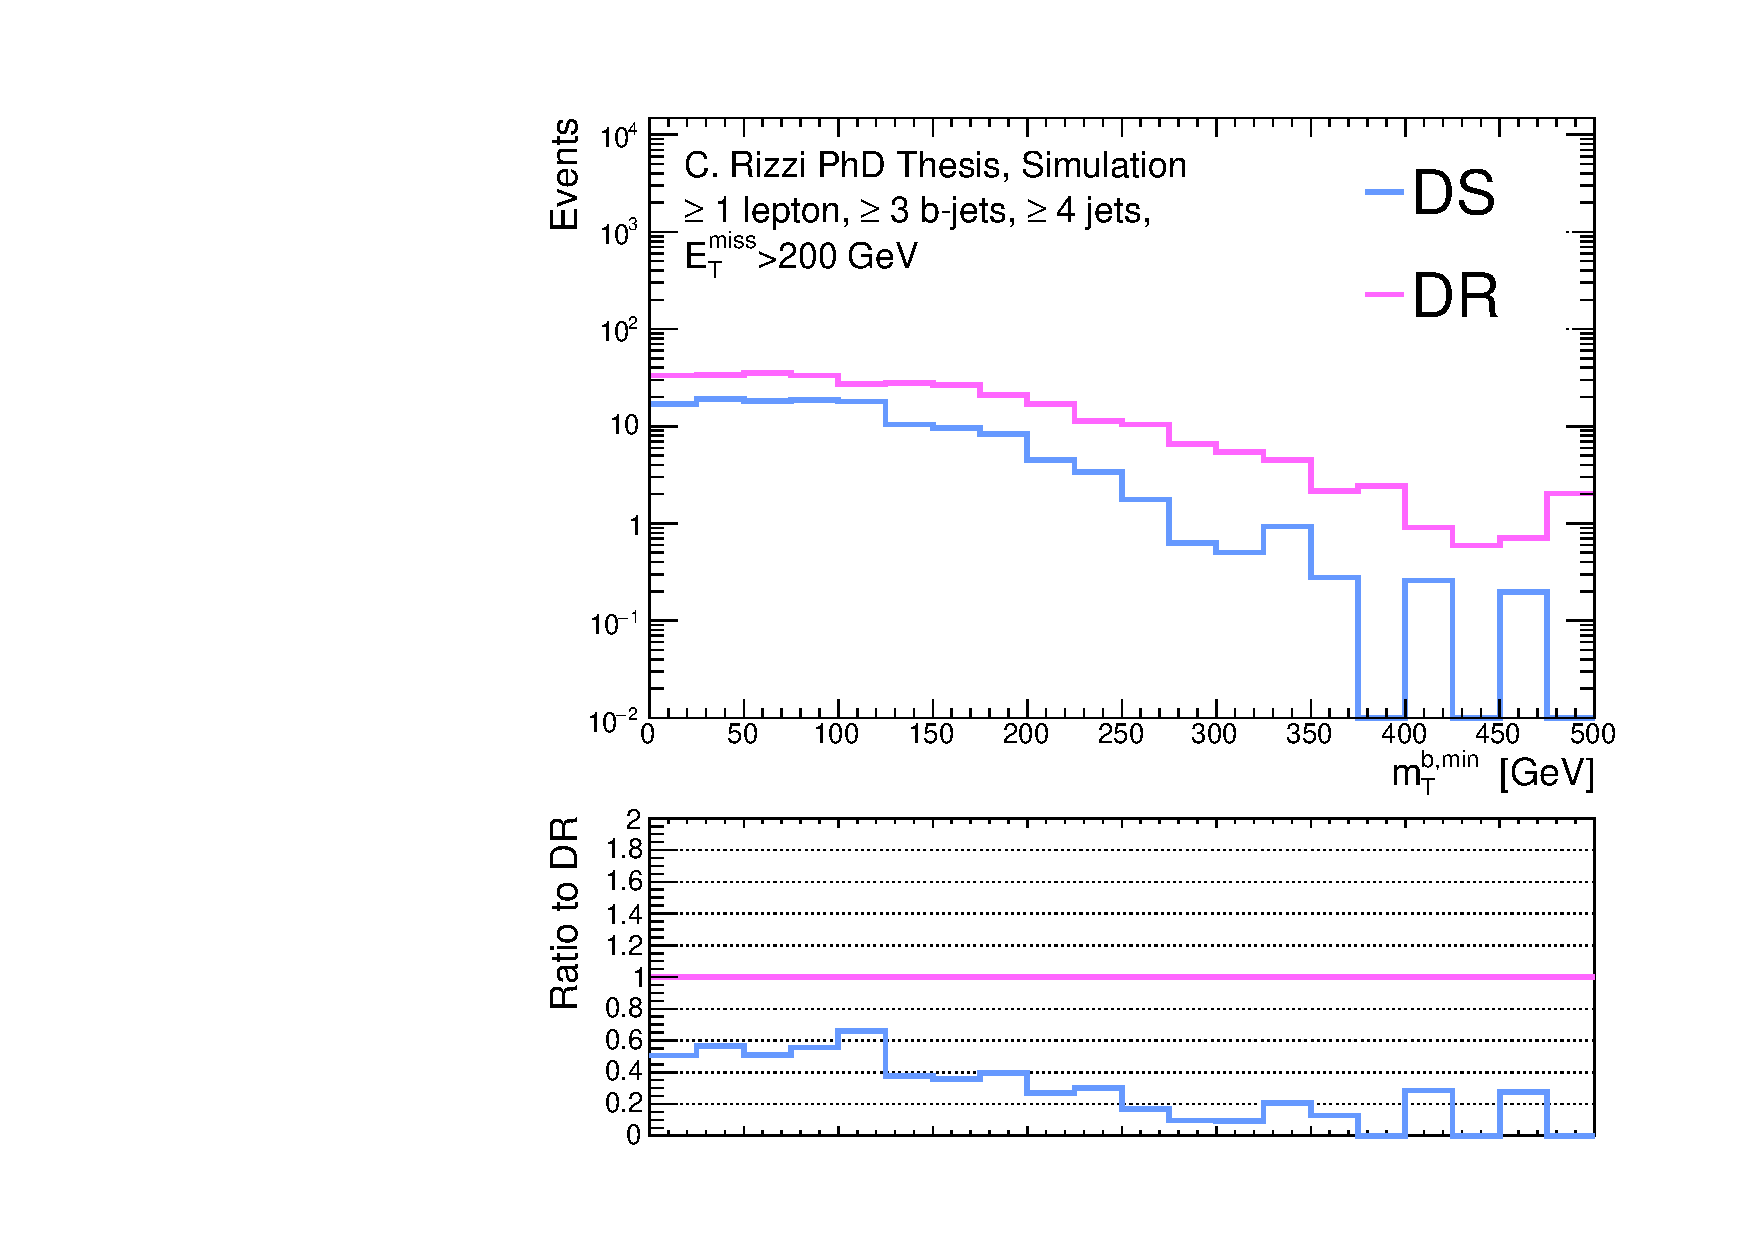
\includegraphics[width=0.32\textwidth]{figures/susy_common/st_DRDS/1L_3b/compare_mTb_min.pdf}\label{fig:st_mtb_1L}}
\subfigure[]{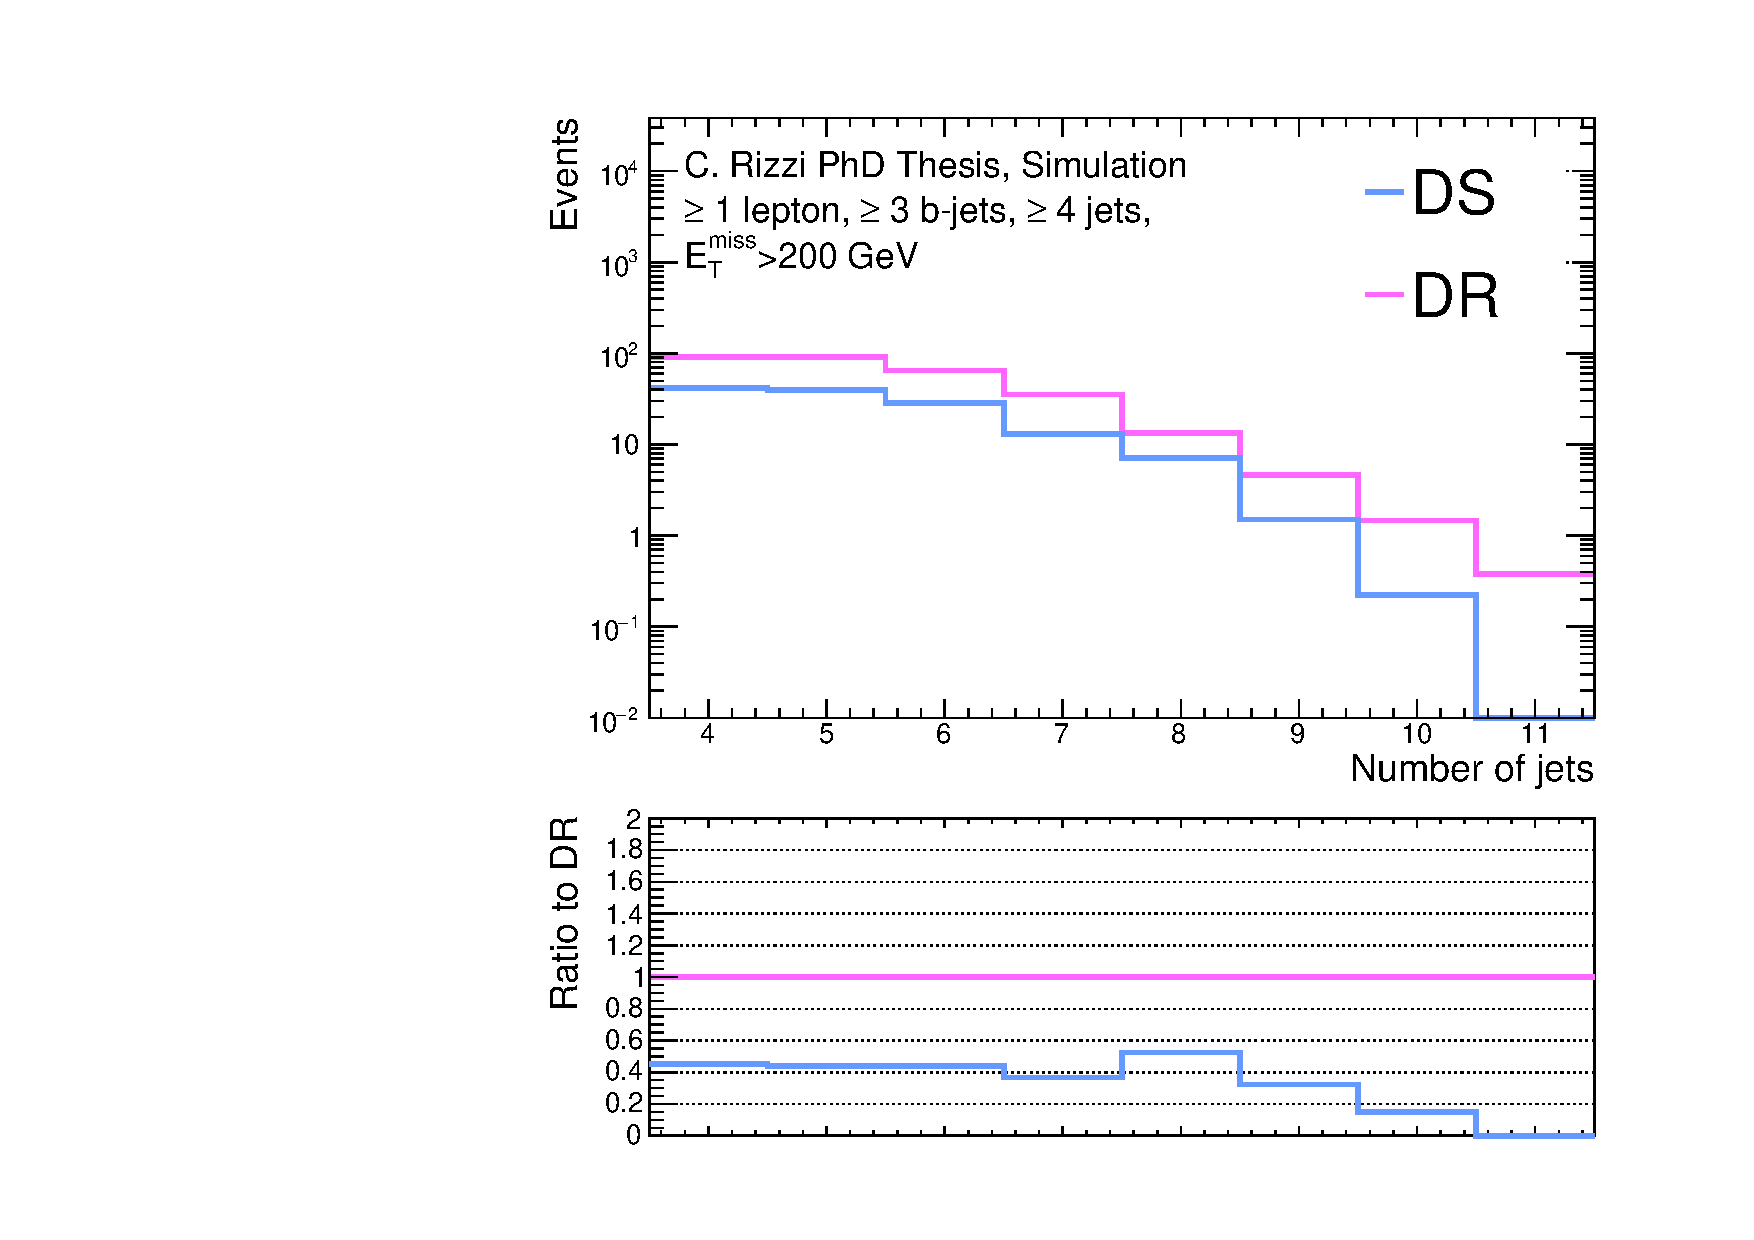
\includegraphics[width=0.32\textwidth]{figures/susy_common/st_DRDS/1L_3b/compare_jets_n.pdf}\label{fig:st_nj_1L}}
\caption{Distribution of \subref{fig:st_met_1L} \met,  \subref{fig:st_mtb_1L} \mtb and \subref{fig:st_nj_1L} number of signal jets in the single top \gls{mc} sample obtained with the \gls{dr} and \gls{ds} approaches (pink and blue line respectively), in a selection requiring at least four jets, at least two $b$-jets, $\met>200$ GeV and at least one lepton. 
}\label{fig:st_1L}
\end{figure}

To evaluate the uncertainty associate with the strategy chosen to account for the interference between \ttbar and single top
we use a dedicated $WWbb$ sample generated at particle level with \aNLO showered with \PY v8, that takes fully into account the interference.
This sample is produced at \gls{lo} and using the four-flavor scheme, where $b$-quarks are treated as massive and processes that require a $b$-quark in the initial state (which is the case for Wt production) are initiated by a gluon splitting into a $b\bar{b}$ pair. 
Because of the \gls{lo} accuracy, the comparison with the sum of the two nominal samples for \ttbar and Wt, generated with \PowhegBox and showered with \PY, does not lead to sensible 
results as the \gls{nlo} corrections to the \ttbar sample are larger than the effect of the interference. 
Instead, two additional samples are generated with the same settings as the $WWbb$ sample to simulate the double-resonance and the single-resonance samples: the former requires the presence of two resonant top quarks, the latter requires one resonant top quark and two $b$-quarks in the \gls{me}, vetoing the presence of a second resonant top quark.  


\subsubsection*{Modelling uncertainties}

The modelling uncertainties on the single top background are estimated at particle level, 
like in the case of the uncertainties on the \ttbar background, but with the difference that in this case the uncertainty is computed based on the difference of expected yields in \glspl{sr} and \glspl{vr} and not based on the difference in the \glspl{tf}; 
this is because in the analyses discussed in this thesis the single top backgrounds is normalized to its theoretical cross section and does not have a data-driven normalization. Truth tagging is used also in this case to increase the available \gls{mc} statistics and to provide a description of the $b$-tagging efficiency closer to the one that we have on reconstructed events. The modelling uncertainties considered are: 

\begin{description}
\item[Interference] The uncertainty deriving from the treatment of the interference between \ttbar and single top in the Wt channel is obtained comparing the sum of single-resonance and double-resonance contributions to the total $WWbb$ sample, using the samples described in the previous paragraph.

\item[Radiation] The systematic uncertainty on the modelling of the extra radiation is estimated with dedicated samples generated with the same set of varied parameters used to generate the variation samples for \ttbar, described in Section \ref{sec:susy_general:ttbar}. 

\end{description}

\subsection{Vector boson in association with jets}

The production of a vector boson ($W$ or $Z$ boson) in association with jets is modeled in \gls{atlas} with the \Sherpa generator in version 2.2: \glspl{me} are 
computed with \comix \cite{Gleisberg:2008fv} and \OL \cite{Cascioli:2011va}, and merged with the \Sherpa parton shower with the CKKW prescription; the \gls{pdf} set used is NNPDF 3.0, and the expected number of events is normalized to the \gls{nnlo} cross-section \cite{Catani:2009sm}.
%For \gls{pp} collisions at 13 TeV, this corresponds to a cross-section of 20080 pb for $W+$jets and 
As an illustration, the \gls{lo} Feynman diagrams for the production of a $W$ boson in association with one jet are shown in Fig. \ref{fig:W_prod}. 
The diagrams for the production of a $Z$ boson in association with one jet are the same, except that in the case of the $Z$ boson the 
two quarks in Fig. \ref{fig:W_prod_1} and the quark and antiquark in Fig. \ref{fig:W_prod_2} have the same flavor. 

\begin{figure}[h]
\centering 
\subfigure[]{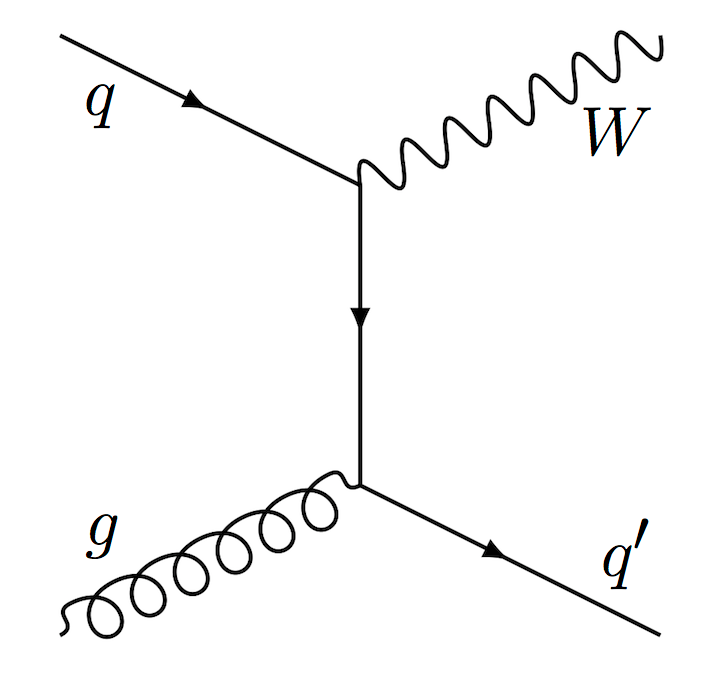
\includegraphics[width=0.25\textwidth]{figures/susy_common/feynman/W_1}\label{fig:W_prod_1}}
\subfigure[]{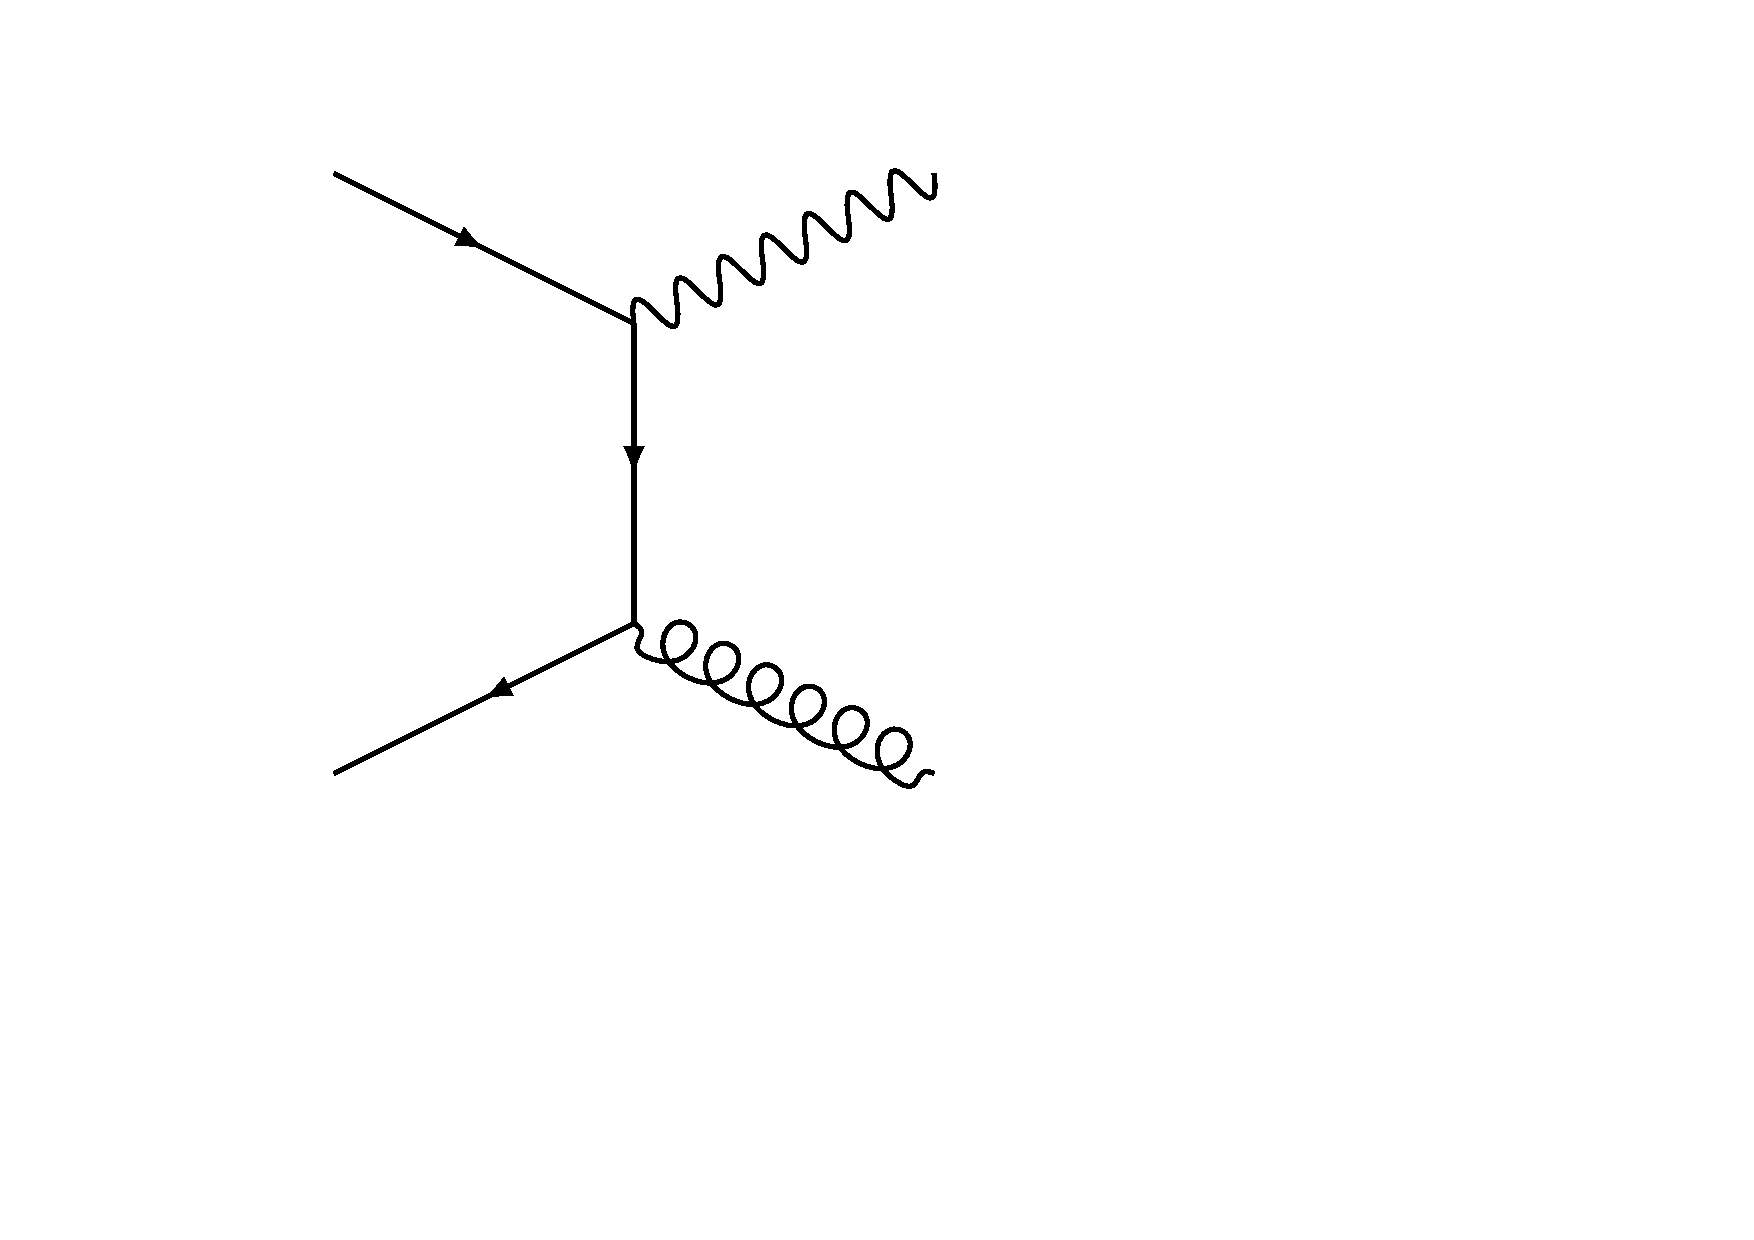
\includegraphics[width=0.25\textwidth]{figures/susy_common/feynman/W_2}\label{fig:W_prod_2}} 
\caption{Representative \gls{lo} Feynman diagrams for the production of a $W$ boson in association with one jet.}\label{fig:W_prod}
\end{figure}

Our analysis selections require high \met and the presence of $b$-jets, therefore most of the $W$+jets events that fulfill the selection are the ones where the $W$ boson decays to a electron, muon or $\tau$ lepton 
and the associated neutrino (to produce some \met) and the $b$-tagging requirement is satisfied because of the production of extra heavy-flavor jets, or because the jet form the hadronic decay of the $\tau$
lepton is incorrectly tagged as a $b$-jet together with other associated jets. 
$W$+jets events can therefore be present both in analysis regions with a lepton requirement and in those with a veto on the presence of leptons. 
In the case of $Z$+jets events, most of the events that enter the analysis regions have a $Z \to \nu \nu$ decay (which has a \gls{br} of about 20\%), and are produced in association with 
heavy-flavor jets or jets that are mistagged; these events contribute almost exclusively to the analysis regions with a lepton veto. 

\subsubsection*{Modeling uncertainties}

The modelling uncertainties considered in the case of the simulation of vector boson production in association with jets are related to the choice of parameters in the \Sherpa generator. 
In particular, the parameters whose choice can influence the description of the events are:

\begin{description}
\item[Renormalization scale] The default renormalization scale ($\mu_{\rm{R}}$) is set to the mass of the $W$ or $Z$ boson in the $W$+jets and $Z$+jets samples respectively. 
The systematic uncertainty associated with this choice is derived by comparison with alternative samples where $\mu_{\rm{R}}$ is set to twice or to half of the nominal value. 

\item[Factorization scale] Like $\mu_{\rm{R}}$, the factorization scale ($\mu_{\rm{F}}$) has its default value at the mass of the vector boson, and is varied to twice and half this value.

\item[Matching scale] The scale for the matching between \gls{me} and \gls{psh} is set to 20 GeV, and this choice is compared with two alternative samples where is set to 30 and 15 GeV.

\item[Resummation scale] As in the case of $\mu_{\rm{R}}$ and $\mu_{\rm{F}}$, the central value of the resummation scale ($Q_{sf}$, the scale used to factorize between constant and logarithmic terms
in the resummation process) is set to the $W$ or $Z$ boson mass, and varied to twice or half its central value in the systematic uncertainties. 

\end{description}

In order to derive the effect of these systematic uncertainties, the analyses described in this thesis do not use a direct comparison of the nominal 
samples with the ones implementing the systematic variations.
Instead, the comparison is implemented through weights with a 2D parametrization based on the number of jets present in the event at particle level 
and on the transverse momentum of the vector boson \cite{Anders:2291836}.
As an example, the impact of these systematic uncertainties on the shapes of the distributions of \met in a selection with a lepton veto is shown in Figure \ref{fig:Z_met_0L_syst} for the $Z$+jets sample and in Figure \ref{fig:W_met_0L_syst} for the $W$+jets sample.  

\begin{figure}[h!]
\centering 
\subfigure[]{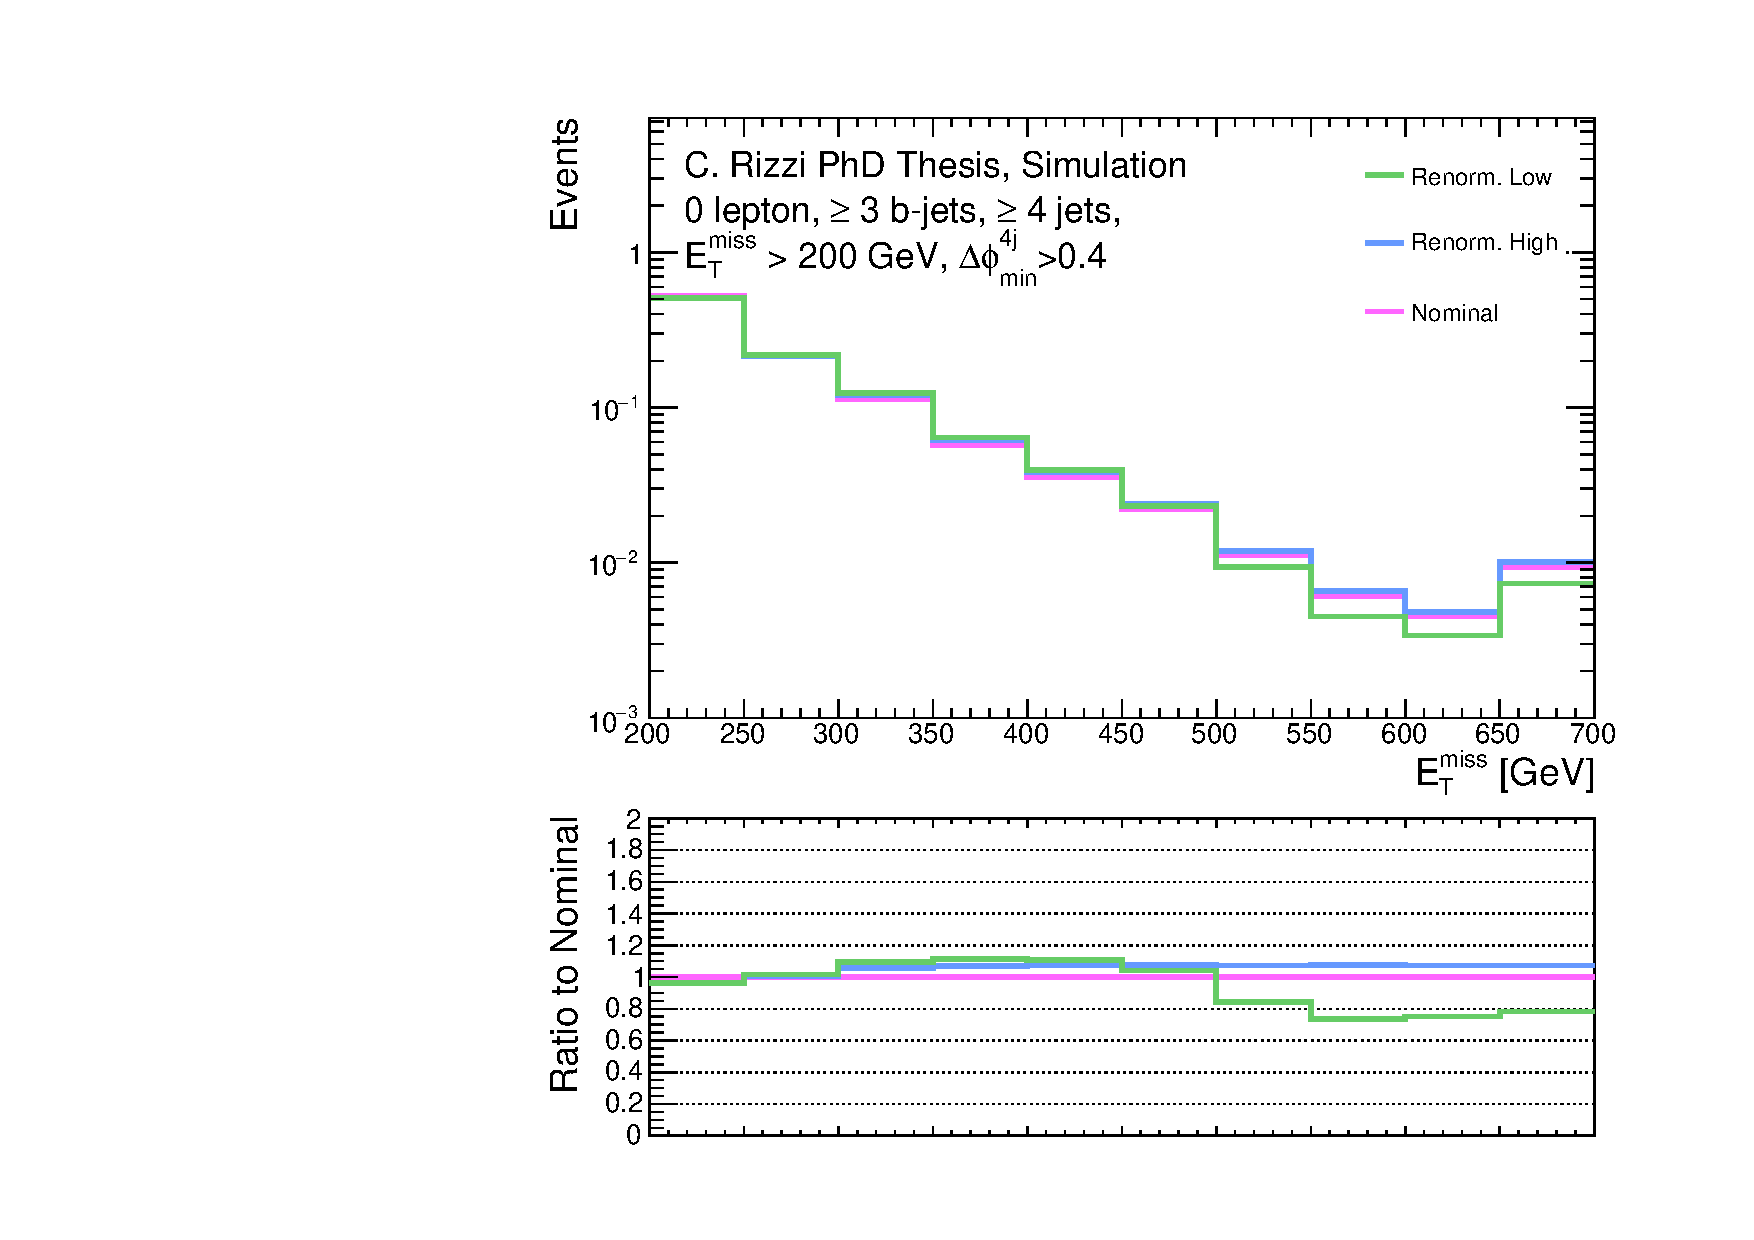
\includegraphics[width=0.32\textwidth]{figures/susy_common/Z_syst_ren/0L_3b/compare_met_Z_scale.pdf}\label{fig:Z_met_0L_ren}}
\subfigure[]{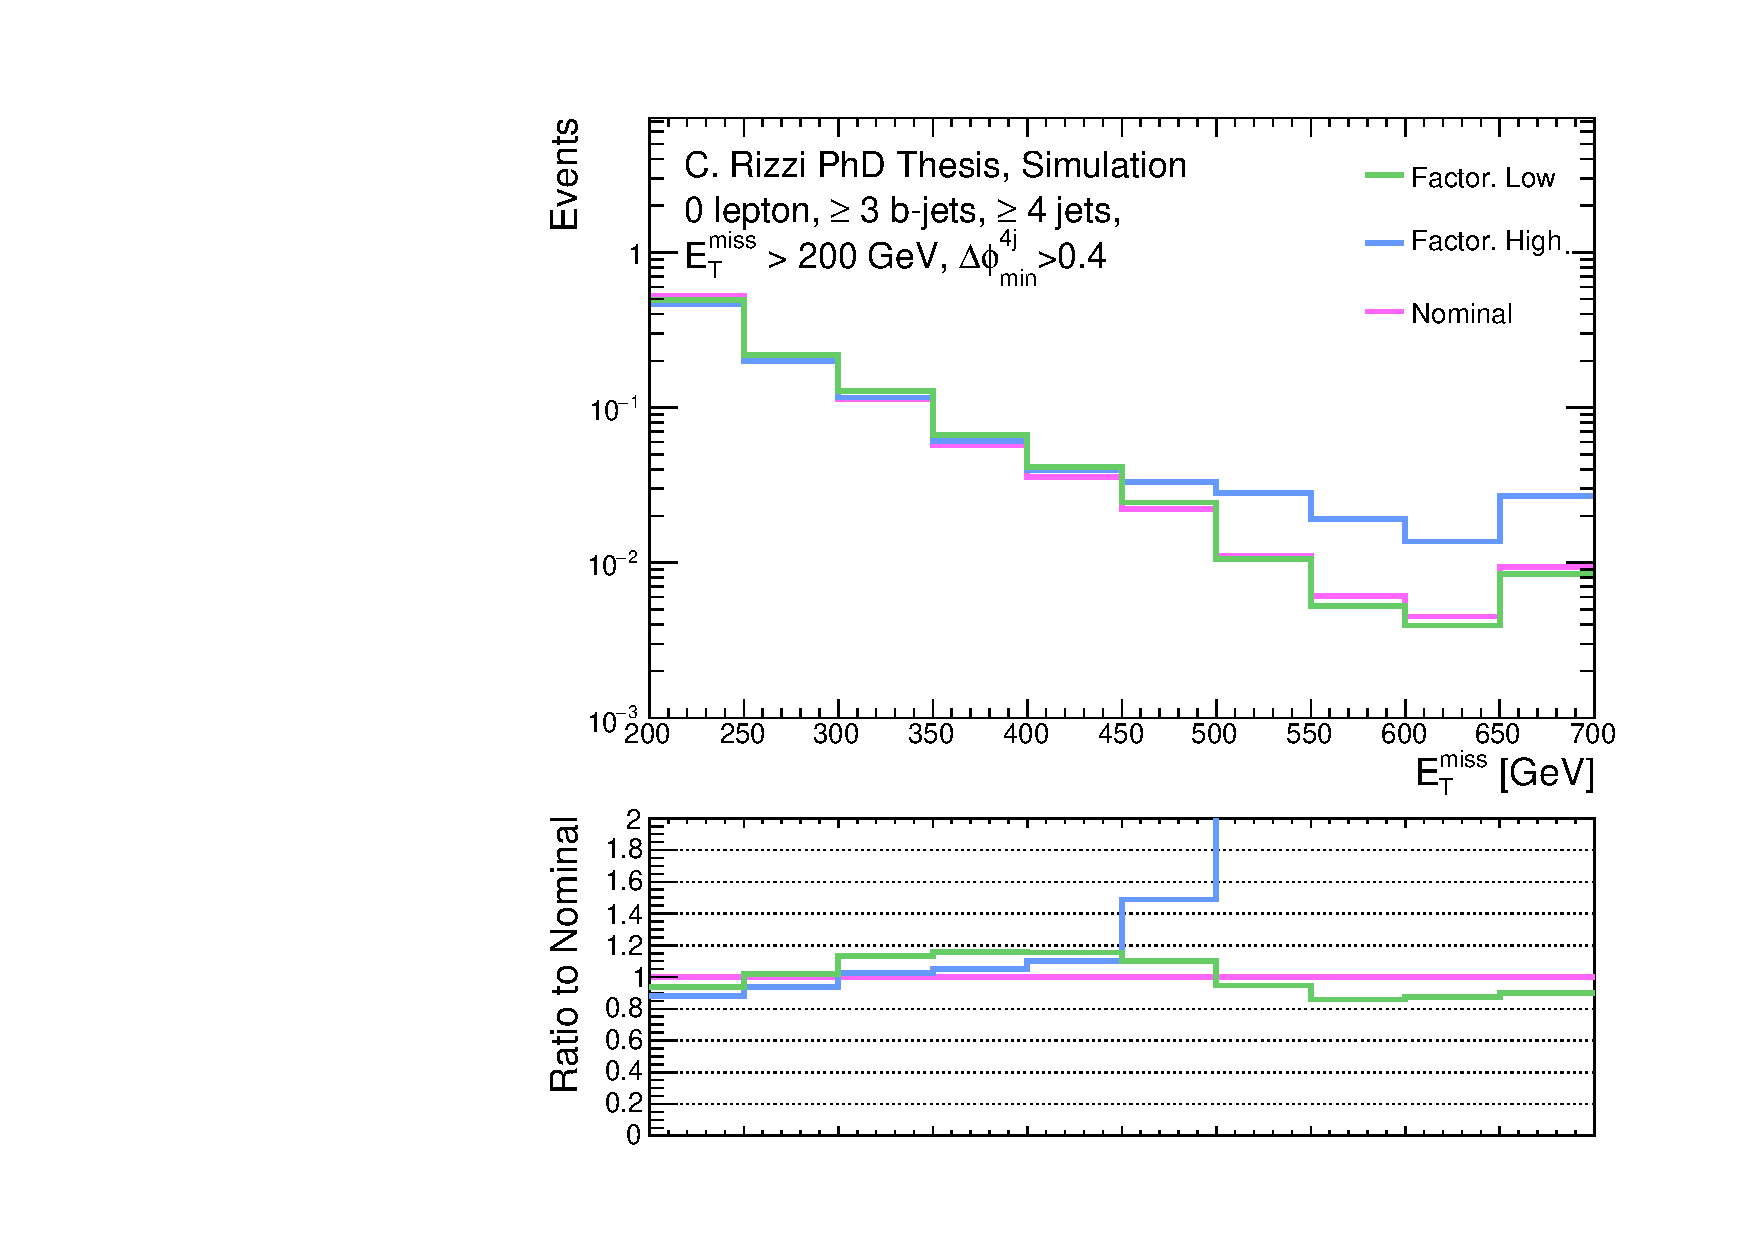
\includegraphics[width=0.32\textwidth]{figures/susy_common/Z_syst_fac/0L_3b/compare_met_Z_scale.pdf}\label{fig:Z_met_0L_fac}}\\
\subfigure[]{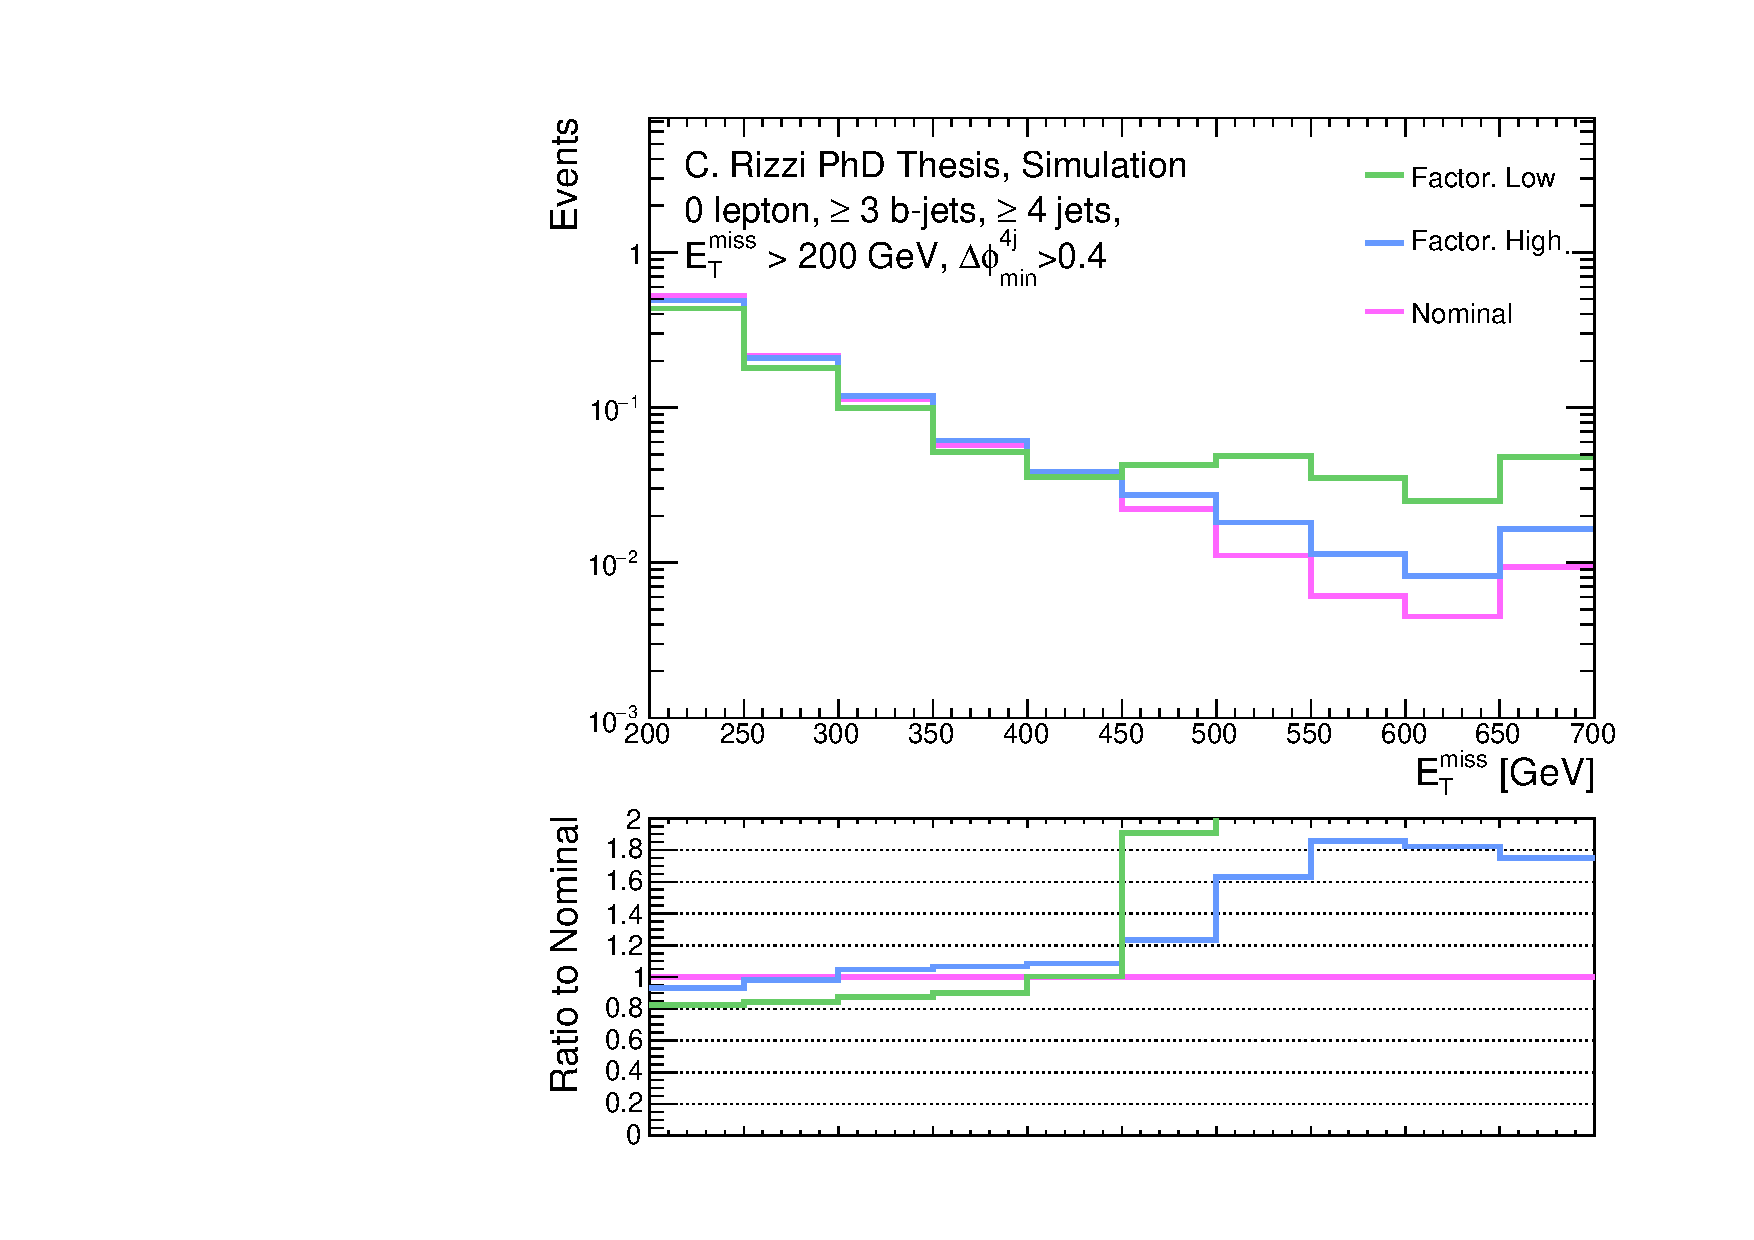
\includegraphics[width=0.32\textwidth]{figures/susy_common/Z_syst_match/0L_3b/compare_met_Z_scale.pdf}\label{fig:Z_met_0L_match}}
\subfigure[]{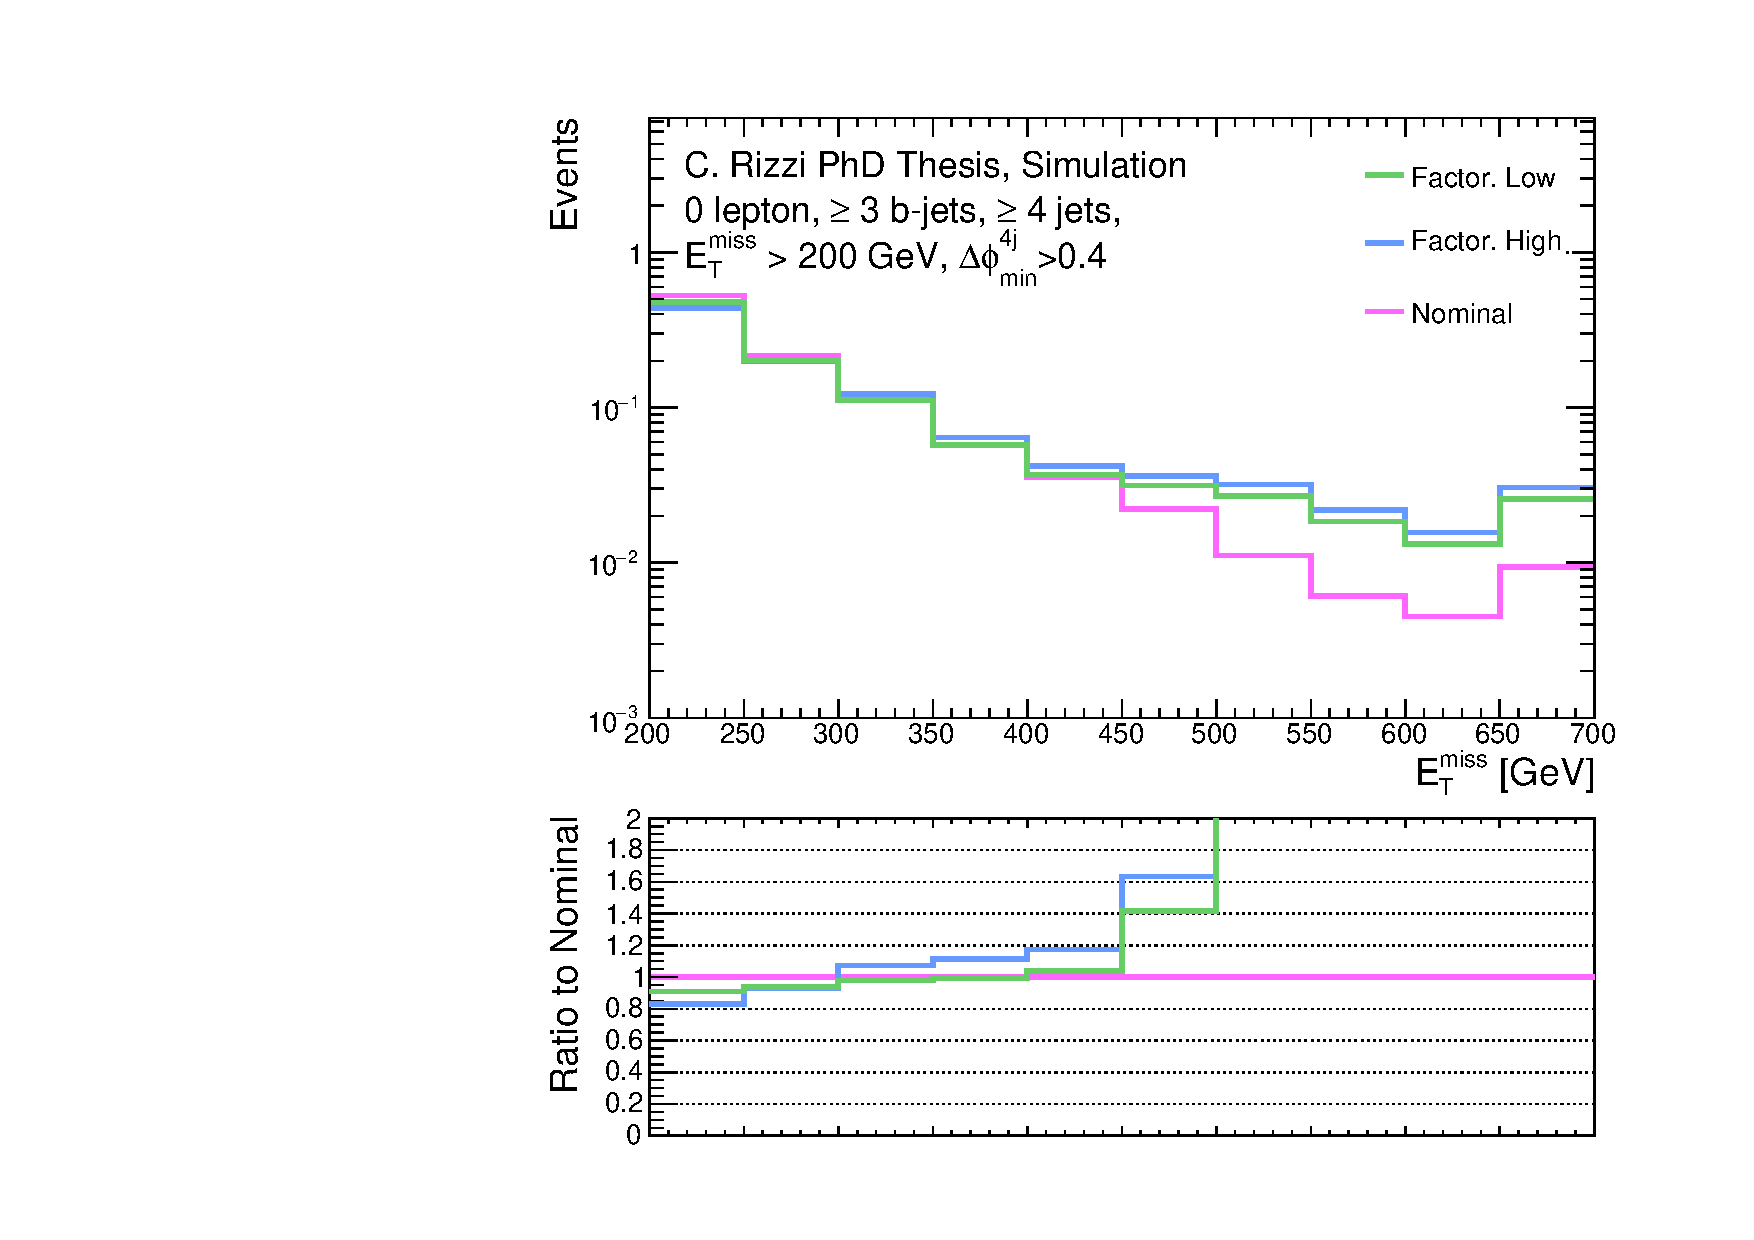
\includegraphics[width=0.32\textwidth]{figures/susy_common/Z_syst_res/0L_3b/compare_met_Z_scale.pdf}\label{fig:Z_met_0L_res}}
\caption{Distribution normalized to unity of the \pt of the leading signal jet in the $Z$+jets \gls{mc} sample in a selection requiring at least four jets, at least two $b$-jets, $\met>200$ GeV and exactly zero lepton. 
\subref{fig:Z_met_0L_ren} Comparison of nominal and renormalization scale variations.
\subref{fig:Z_met_0L_fac} Comparison of nominal and factorization scale variations.
\subref{fig:Z_met_0L_match} Comparison of nominal and matching scale variations.
\subref{fig:Z_met_0L_res} Comparison of nominal and resummation scale variations.
}\label{fig:Z_met_0L_syst}
\end{figure}

\begin{figure}[h!]
\centering 
\subfigure[]{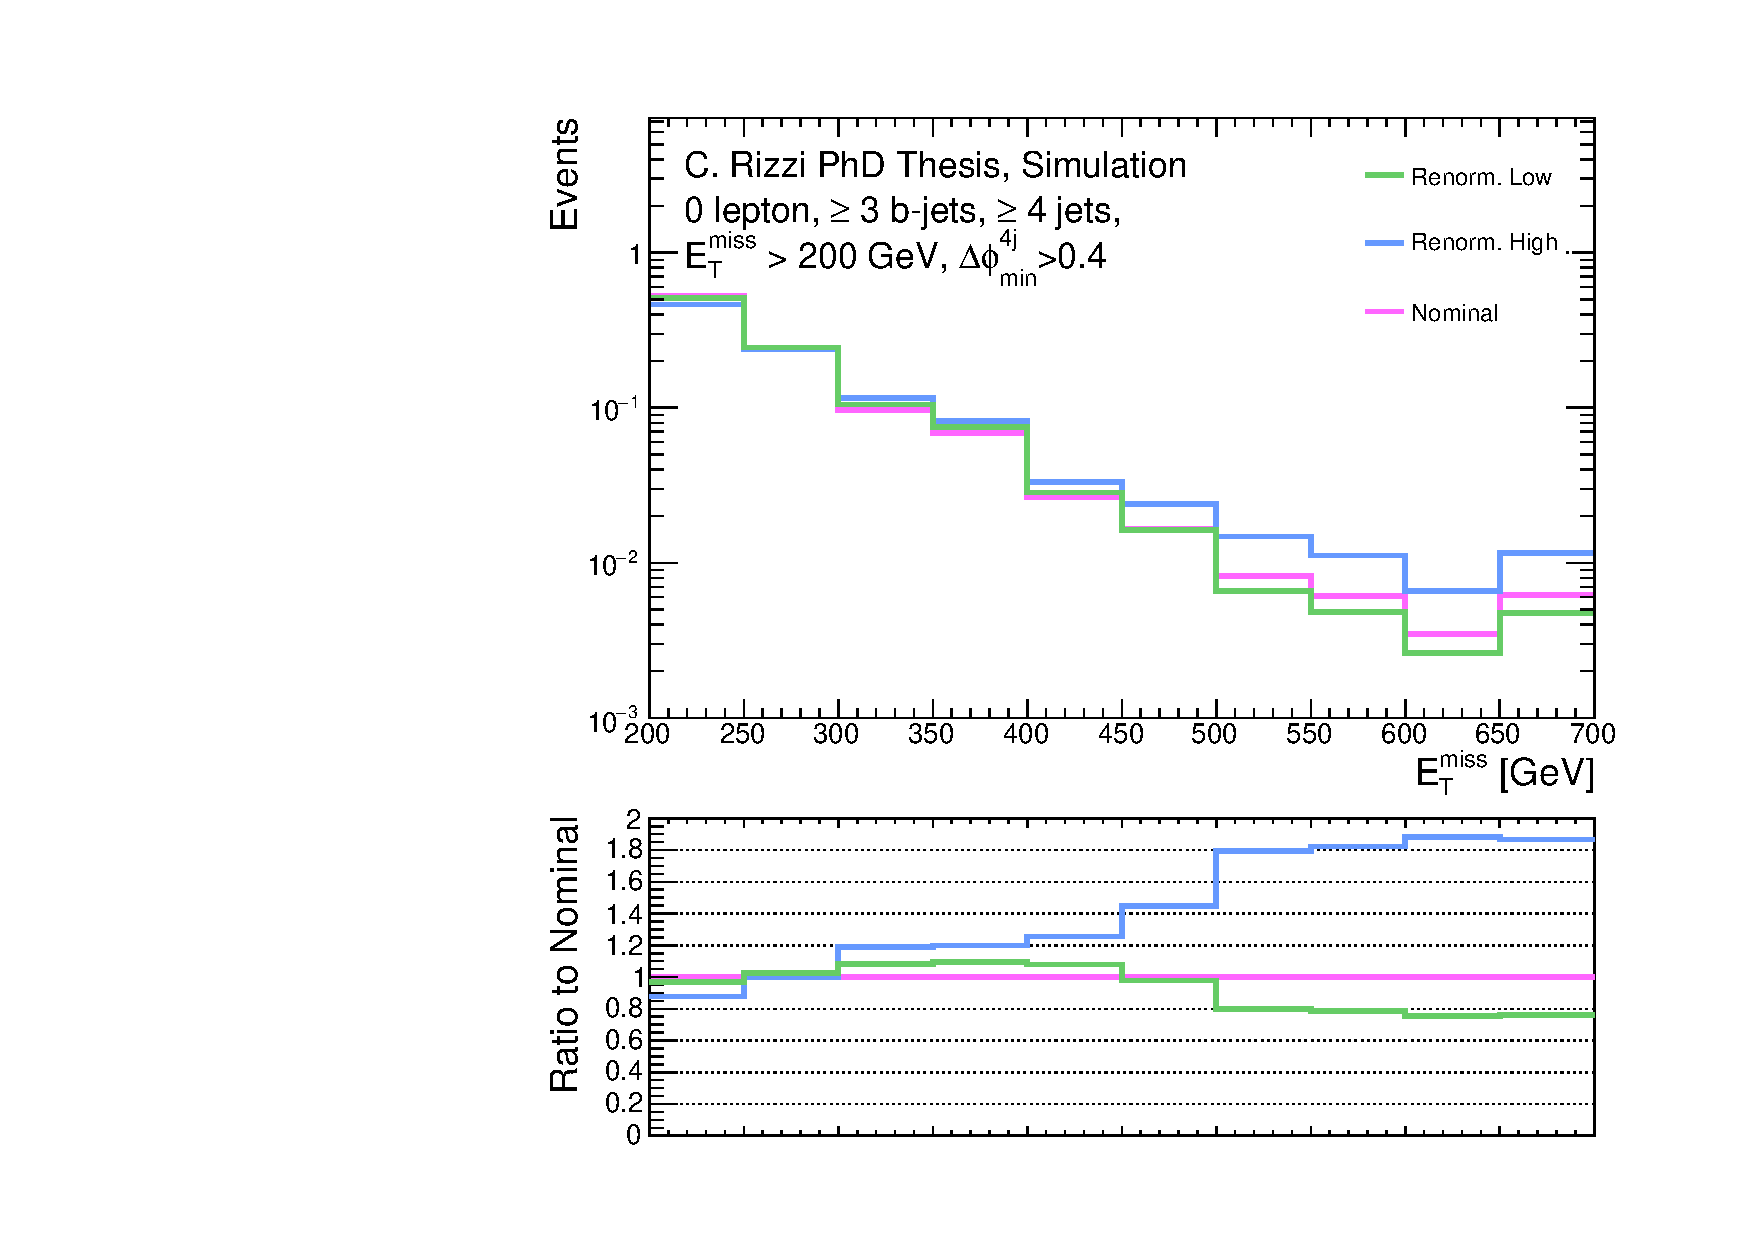
\includegraphics[width=0.32\textwidth]{figures/susy_common/W_syst_ren/0L_3b/compare_met_W_scale.pdf}\label{fig:W_met_0L_ren}}
\subfigure[]{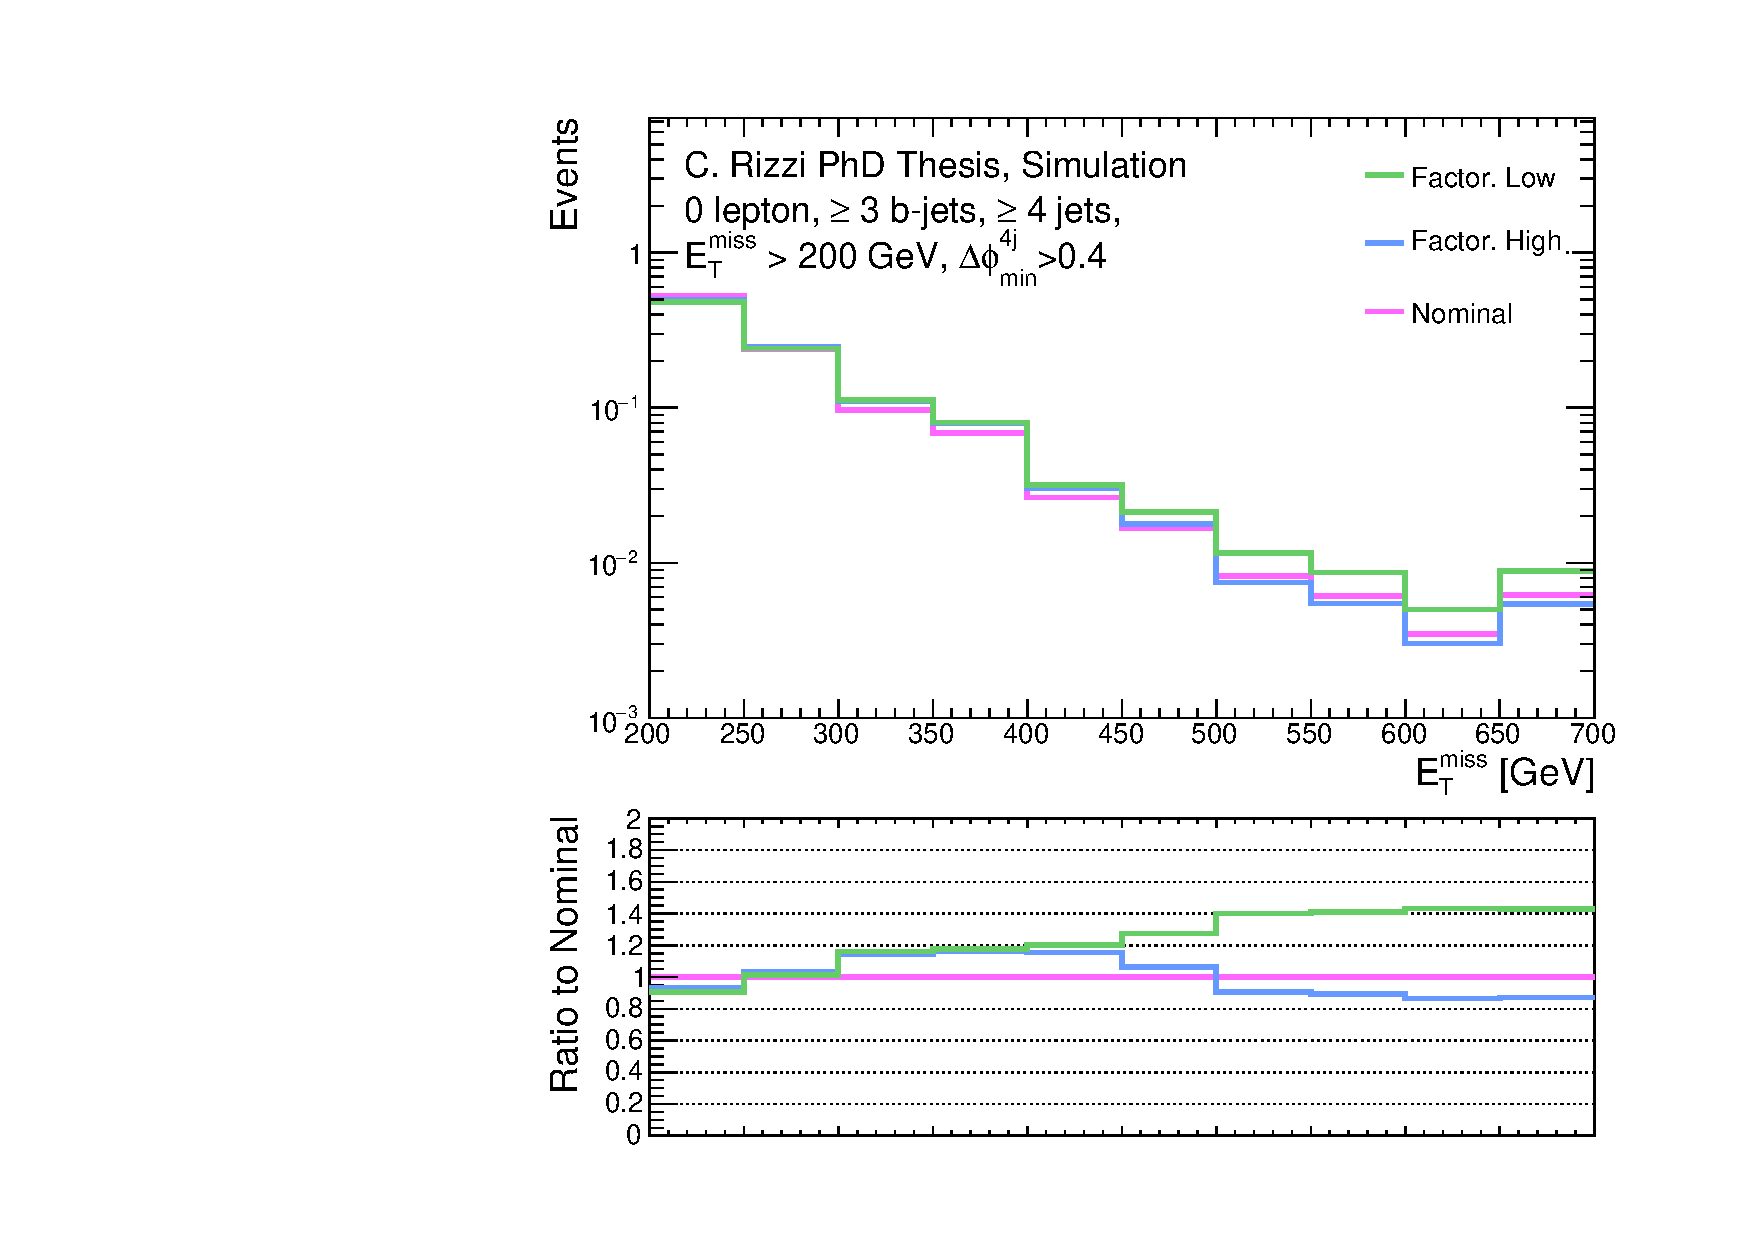
\includegraphics[width=0.32\textwidth]{figures/susy_common/W_syst_fac/0L_3b/compare_met_W_scale.pdf}\label{fig:W_met_0L_fac}}\\
\subfigure[]{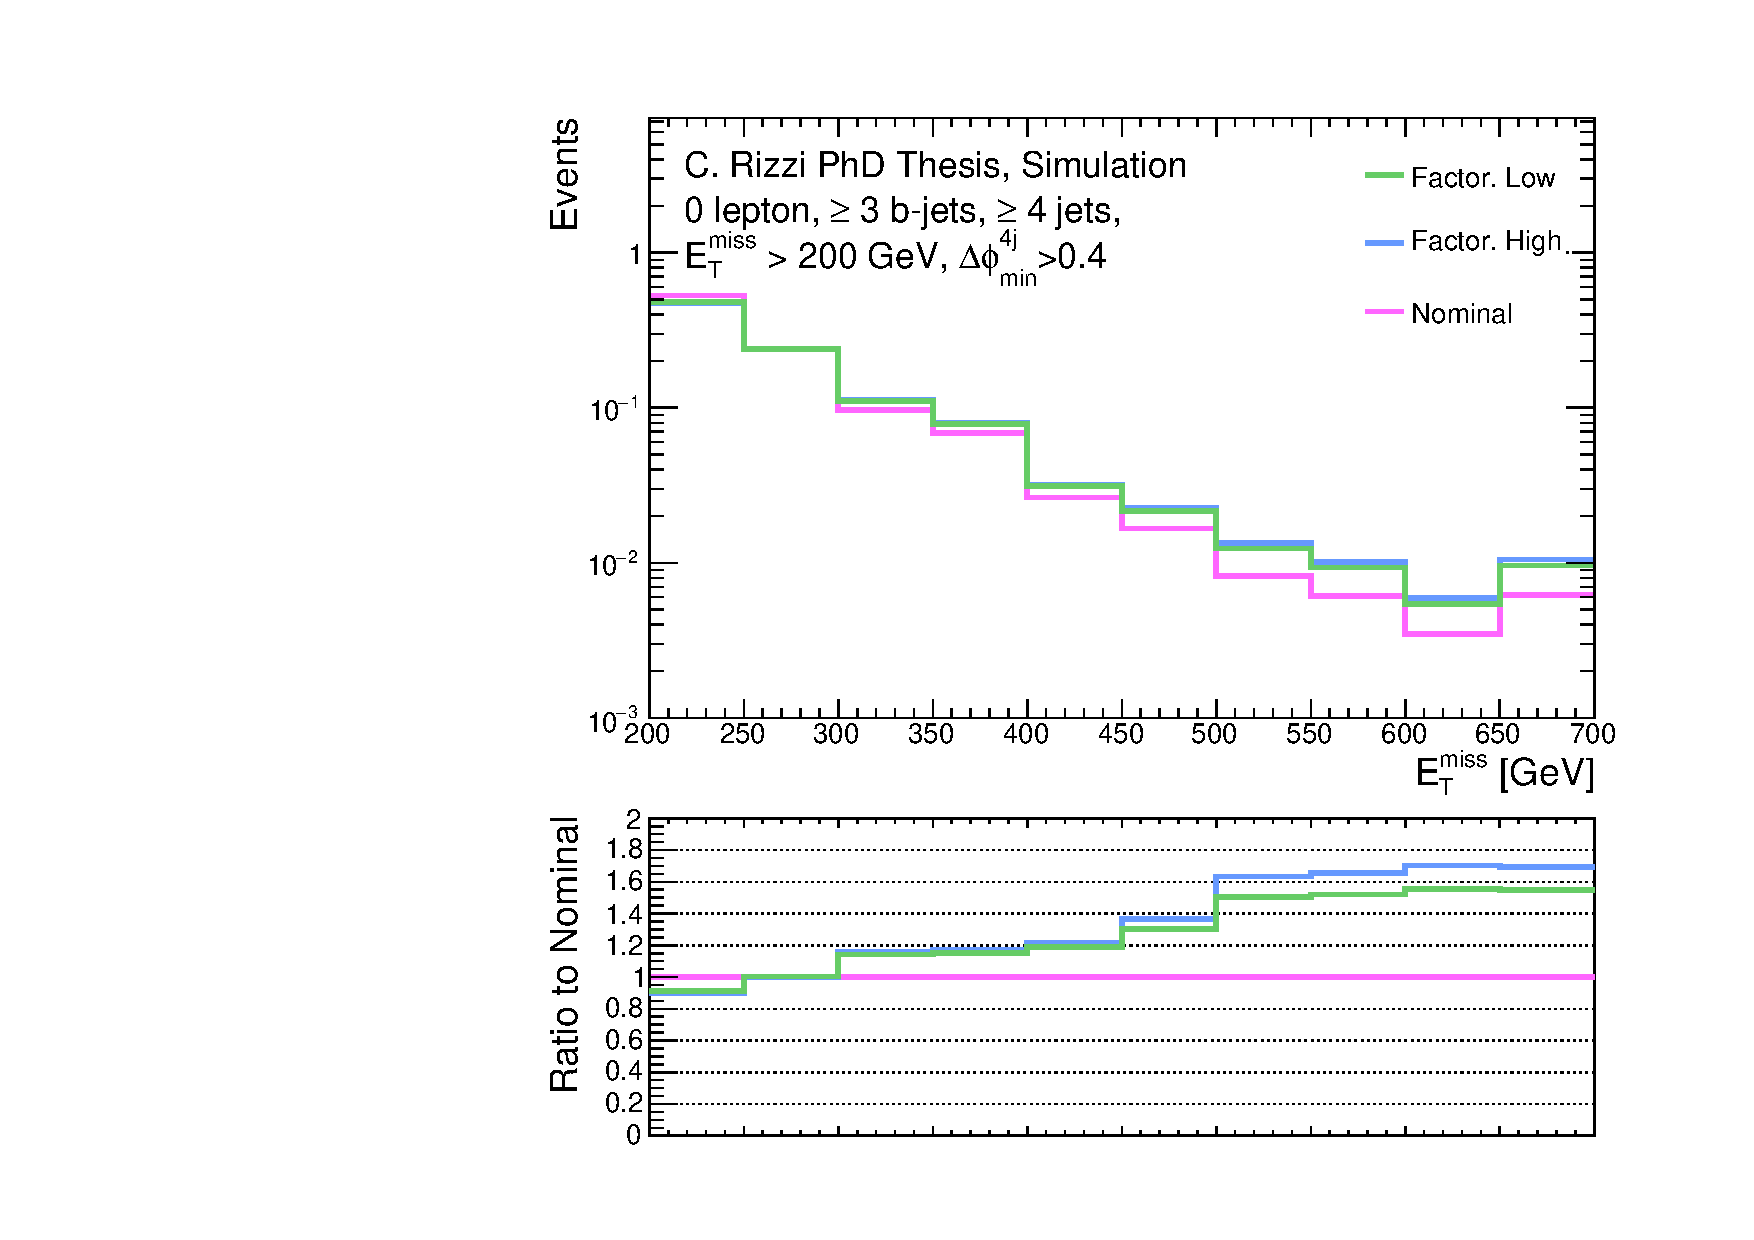
\includegraphics[width=0.32\textwidth]{figures/susy_common/W_syst_match/0L_3b/compare_met_W_scale.pdf}\label{fig:W_met_0L_match}}
\subfigure[]{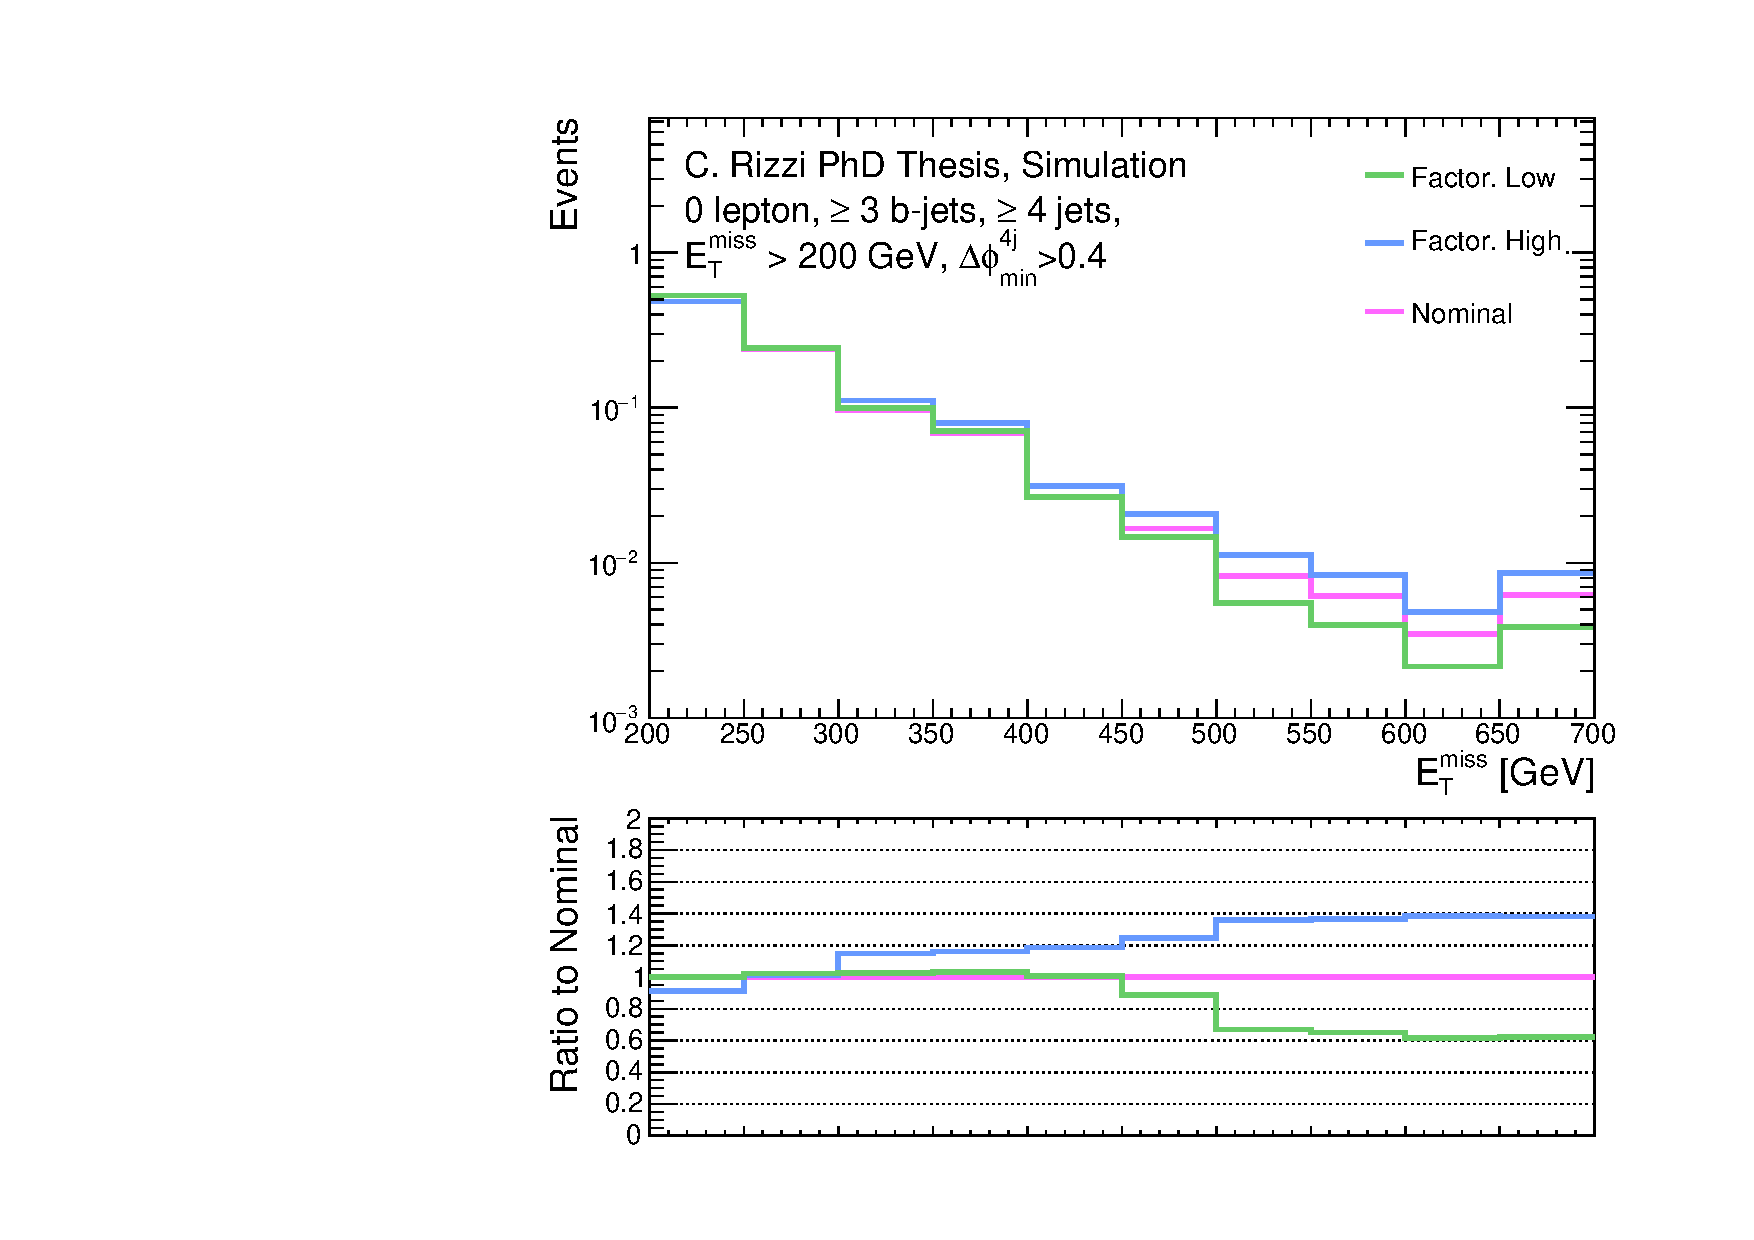
\includegraphics[width=0.32\textwidth]{figures/susy_common/W_syst_res/0L_3b/compare_met_W_scale.pdf}\label{fig:W_met_0L_res}}
\caption{Distribution normalized to unity of the \pt of the leading signal jet in the $Z$+jets \gls{mc} sample in a selection requiring at least four jets, at least two $b$-jets, $\met>200$ GeV and exactly zero lepton. 
\subref{fig:W_met_0L_ren} Comparison of nominal and renormalization scale variations.
\subref{fig:W_met_0L_fac} Comparison of nominal and factorization scale variations.
\subref{fig:W_met_0L_match} Comparison of nominal and matching scale variations.
\subref{fig:W_met_0L_res} Comparison of nominal and resummation scale variations.
}\label{fig:W_met_0L_syst}
\end{figure}


\subsection{Diboson production}

Beside the production of a single vector boson, also pair production is possible: 
the \gls{lo} Feynman diagrams for the production of a boson pair are shown in Fig. \ref{fig:dib_prod}.
The cross-section is suppressed by more than three orders of magnitude with respect to the 
single-vector-boson case. 
Therefore, despite that presence of two bosons leads a higher acceptance into the analysis regions,
the overall contribution diboson processes to the total \gls{sm} background is small. 
The diboson \gls{mc} samples are generated with \Sherpa v2.2.1, and their cross sections are computed at \gls{nlo} \cite{ATL-PHYS-PUB-2016-002,ATL-PHYS-PUB-2017-005}.
A 50\% normalization uncertainty is applied to the predicted number of events for this background, to take into account 
systematic uncertainties on its modelling. This conservative uncertainty is found to have a negligible impact in the analysis results. 


\begin{figure}[h!]
\centering 
\subfigure[]{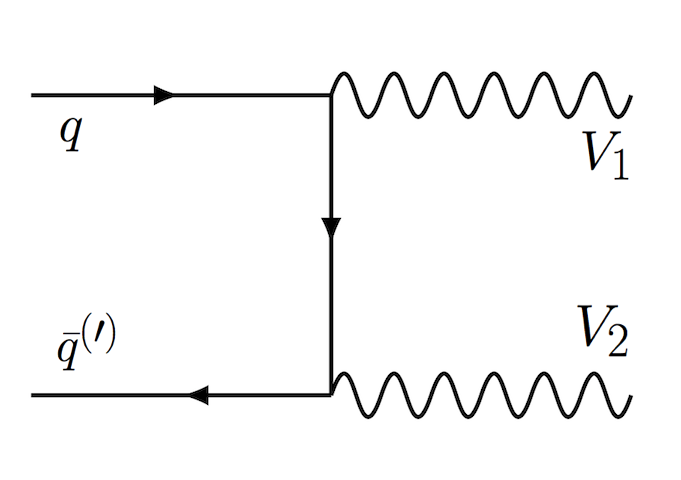
\includegraphics[width=0.3\textwidth]{figures/susy_common/feynman/dib_1}\label{fig:dib_prod_1}}
\subfigure[]{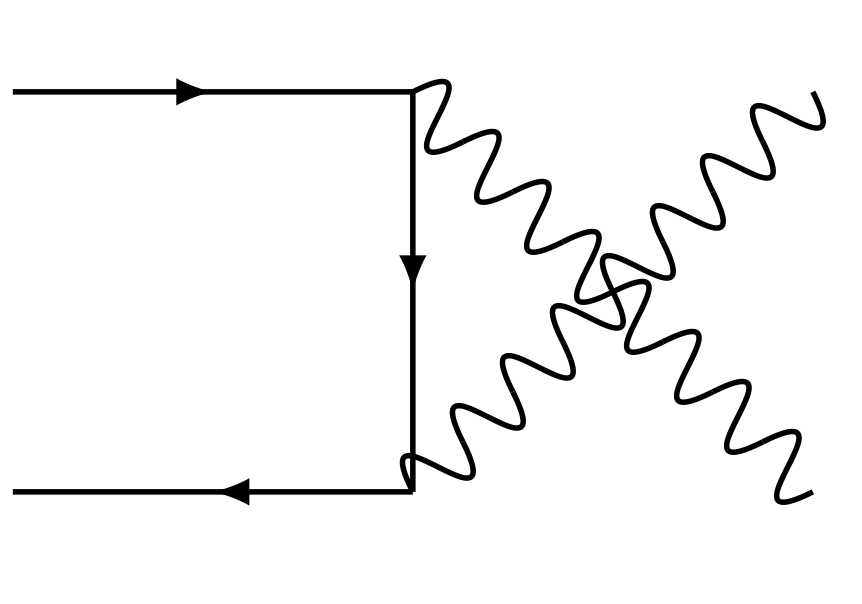
\includegraphics[width=0.3\textwidth]{figures/susy_common/feynman/dib_2}\label{fig:dib_prod_2}} 
\subfigure[]{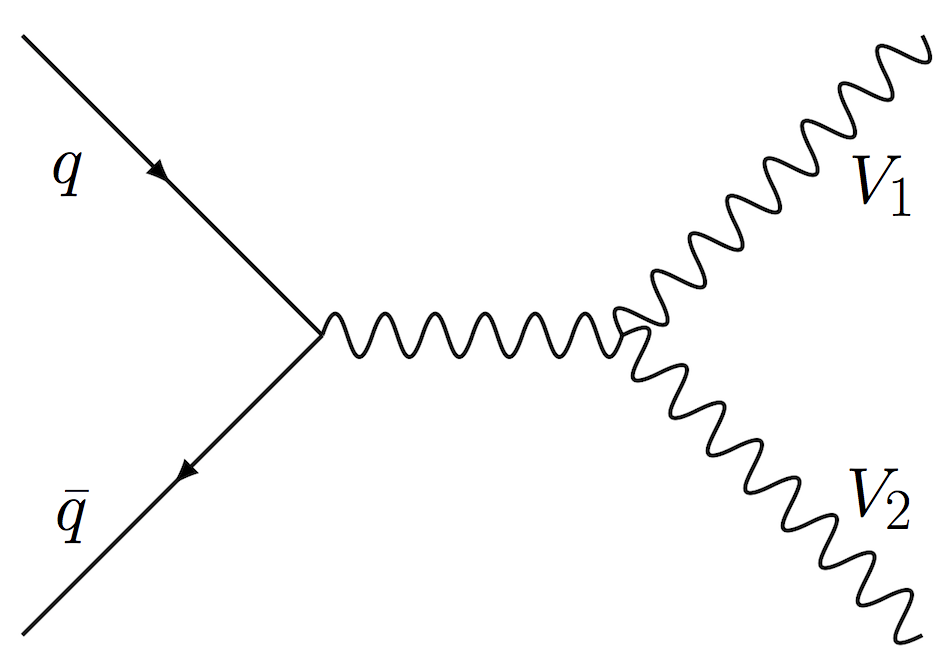
\includegraphics[width=0.3\textwidth]{figures/susy_common/feynman/dib_3}\label{fig:dib_prod_3}}
\caption{Representative \gls{lo} Feynman diagrams for diboson production  ($V=W, Z$).}\label{fig:dib_prod}
\end{figure}


\subsection{\ttbar + X production}

A pair of top quarks can be produced also in association with a vector boson o a Higgs boson, as shown in Figures \ref{fig:ttW_prod}-\ref{fig:tth_prod}.
In this thesis, these processes constitute a minor background and are grouped in the category $\ttbar+X$, together with four-top production,
for which an example \gls{lo} Feynman diagram is shown in Figure \ref{fig:fourtop_prod}. 
The production of a \ttbar pair in association with a vector boson and four-top production is modeled with \aNLO showered with \PY v8, while for $\ttbar+H$ the same 
\gls{me} generator is used but the \gls{psh} processes is performed with \HWpp. 
All of these samples are normalized to the \gls{nlo} cross-section \cite{Alwall:2014hca,Heinemeyer:2013tqa}.
As described above for the diboson background, a conservative 50\% normalization uncertainty is applied also to the 
$\ttbar+X$ background, and also in this case it is found to have negligible impact in the analysis. 

\begin{figure}[h!]
\centering 
\subfigure[]{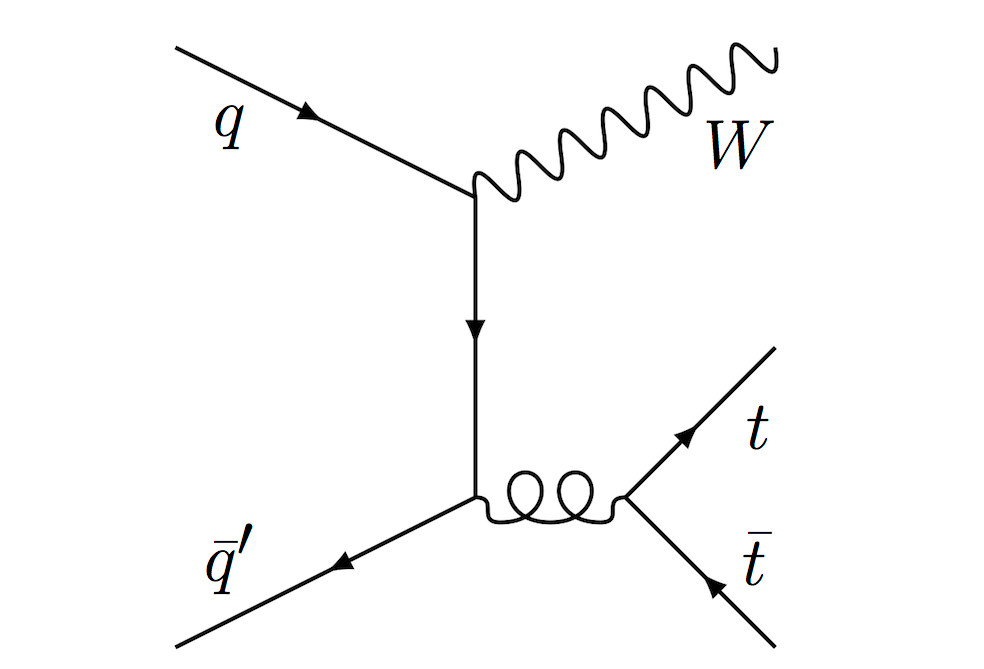
\includegraphics[width=0.3\textwidth]{figures/susy_common/feynman/ttW}\label{fig:ttW_prod}}
\subfigure[]{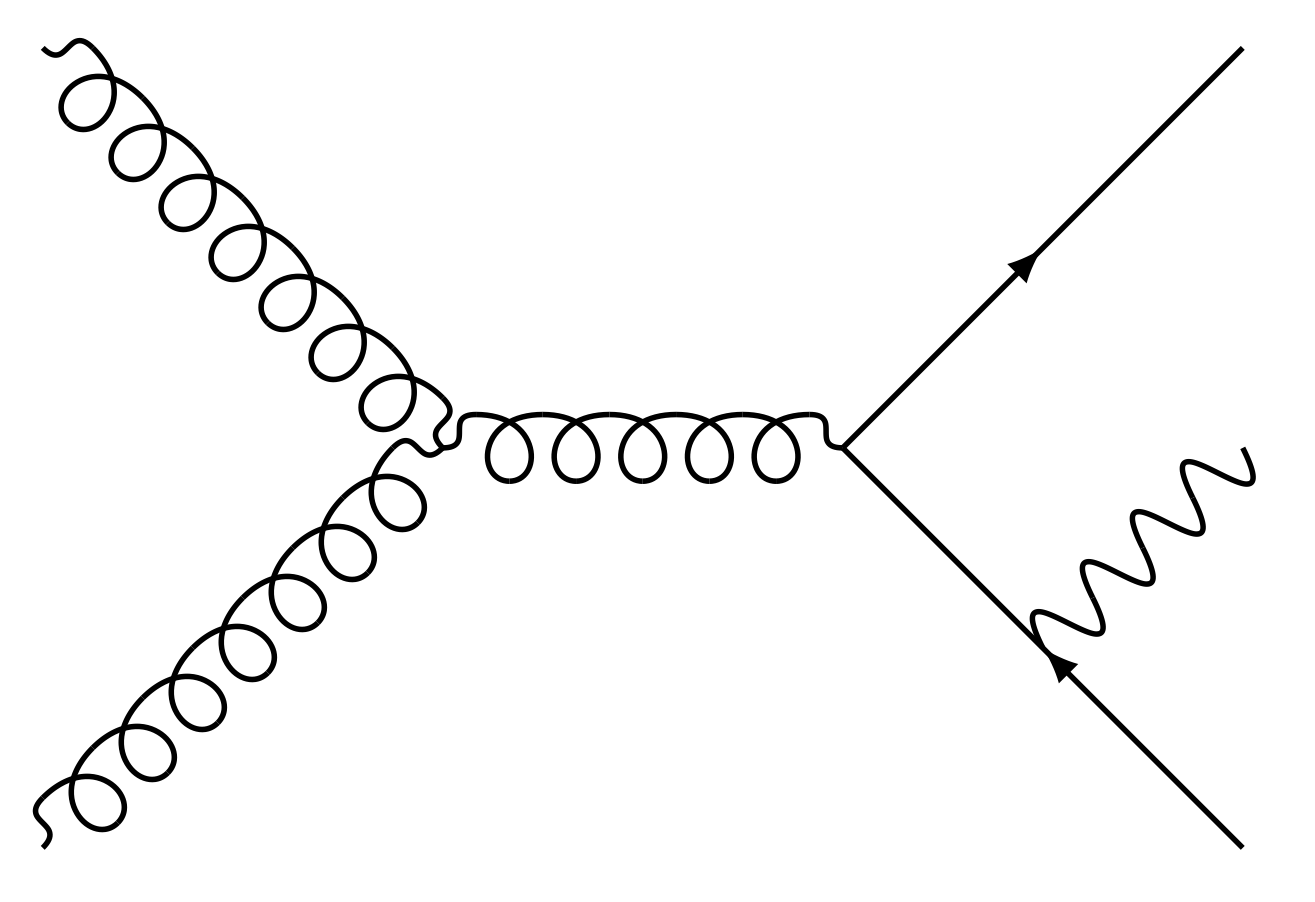
\includegraphics[width=0.3\textwidth]{figures/susy_common/feynman/ttZ}\label{fig:ttZ_prod}} \\
\subfigure[]{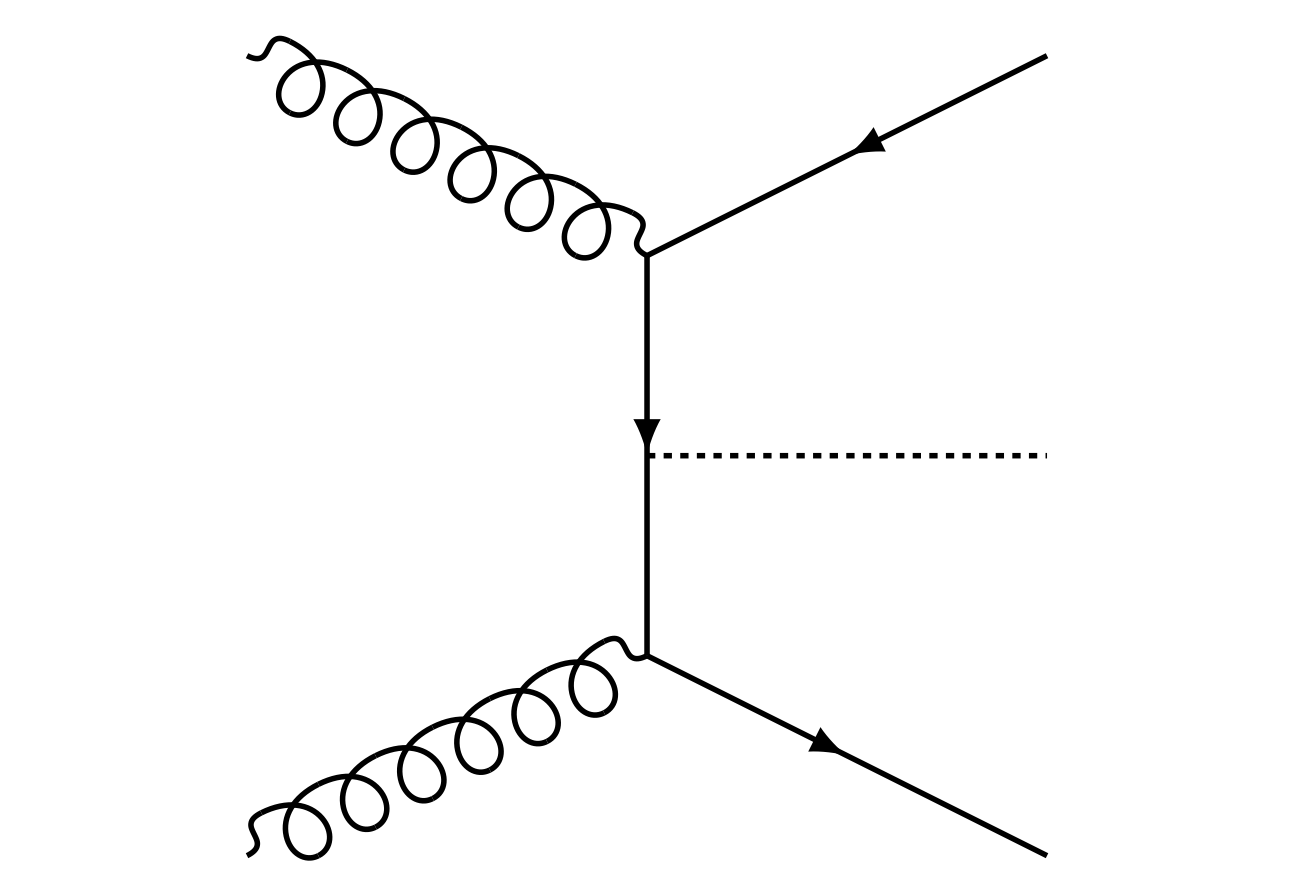
\includegraphics[width=0.3\textwidth]{figures/susy_common/feynman/tth}\label{fig:tth_prod}}
\subfigure[]{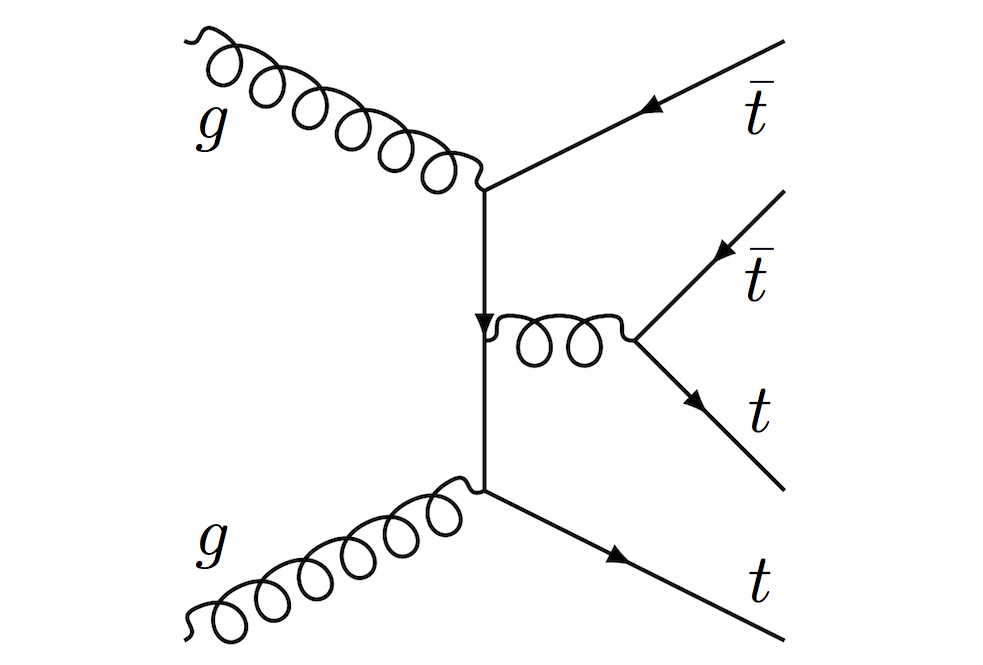
\includegraphics[width=0.3\textwidth]{figures/susy_common/feynman/fourtop}\label{fig:fourtop_prod}}
\caption{Representative \gls{lo} Feynman diagram for the production of \subref{fig:ttW_prod} $t\bar{t}W$, \subref{fig:ttZ_prod} $t\bar{t}Z$, \subref{fig:tth_prod} $t\bar{t}H$, and \subref{fig:fourtop_prod} \fourtop.}\label{fig:ttX_prod}
\end{figure}

\subsection{QCD multijet}

Multijet production is by far the process with the largest cross-section at the \gls{lhc} ($\mathcal{O}$(mb)). 
Most of the \gls{qcd} events are $2 \to 2$ processes, for which some example \gls{lo} Feynman diagrams are shown in Fig. \ref{fig:qcd_prod_1} and Fig \ref{fig:qcd_prod_2}, but higher order processes ($2 \to n$) are possible as well (an example of $2 \to 3$ process is shown in Fig. \ref{fig:qcd_prod_3}). 
Multijet processes do not have real \met, and therefore they can be a background in analyses that require high \met only if one or more of the jets are mismeasured, leading to an energy imbalance in the transverse plane that is reconstructed as \met. 
These processes do not produce any lepton either, so also a contribution to analyses requiring leptons must originate from a jet misreconstructed as a lepton. 
Since the probability for a multijet event to both have a fake high \met and a fake lepton is very small, multijet processes are considered as background only in the analysis regions with a veto on the presence of leptons. 


\begin{figure}[h!]
\centering 
\subfigure[]{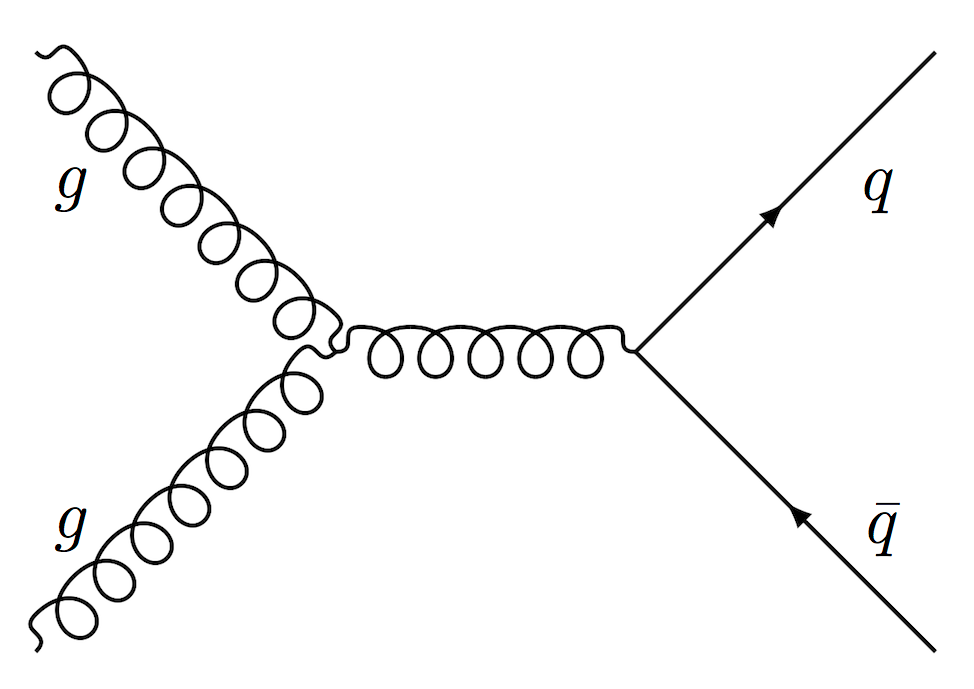
\includegraphics[width=0.3\textwidth]{figures/susy_common/feynman/qcd_1}\label{fig:qcd_prod_1}}
\subfigure[]{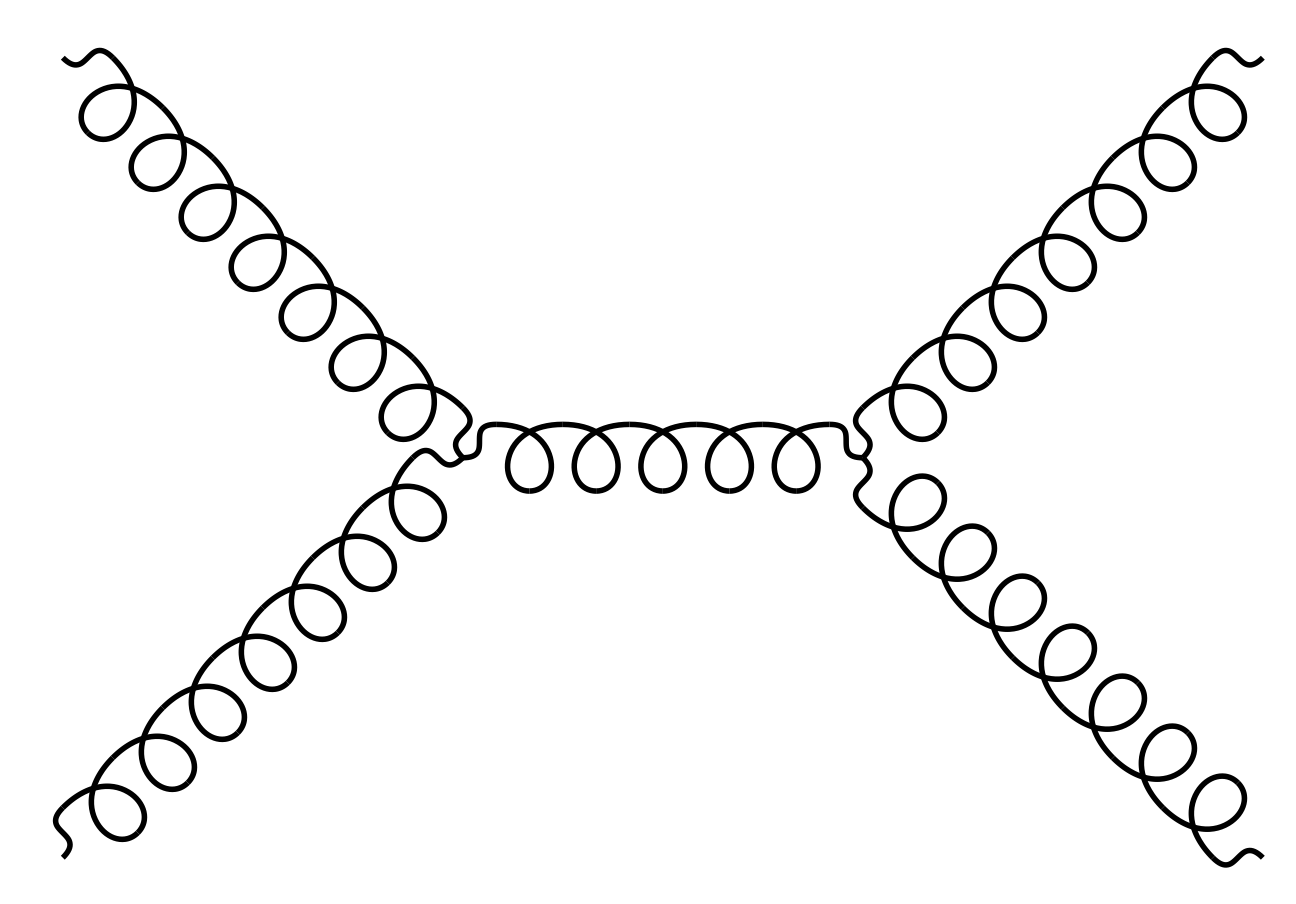
\includegraphics[width=0.3\textwidth]{figures/susy_common/feynman/qcd_2}\label{fig:qcd_prod_2}} 
\subfigure[]{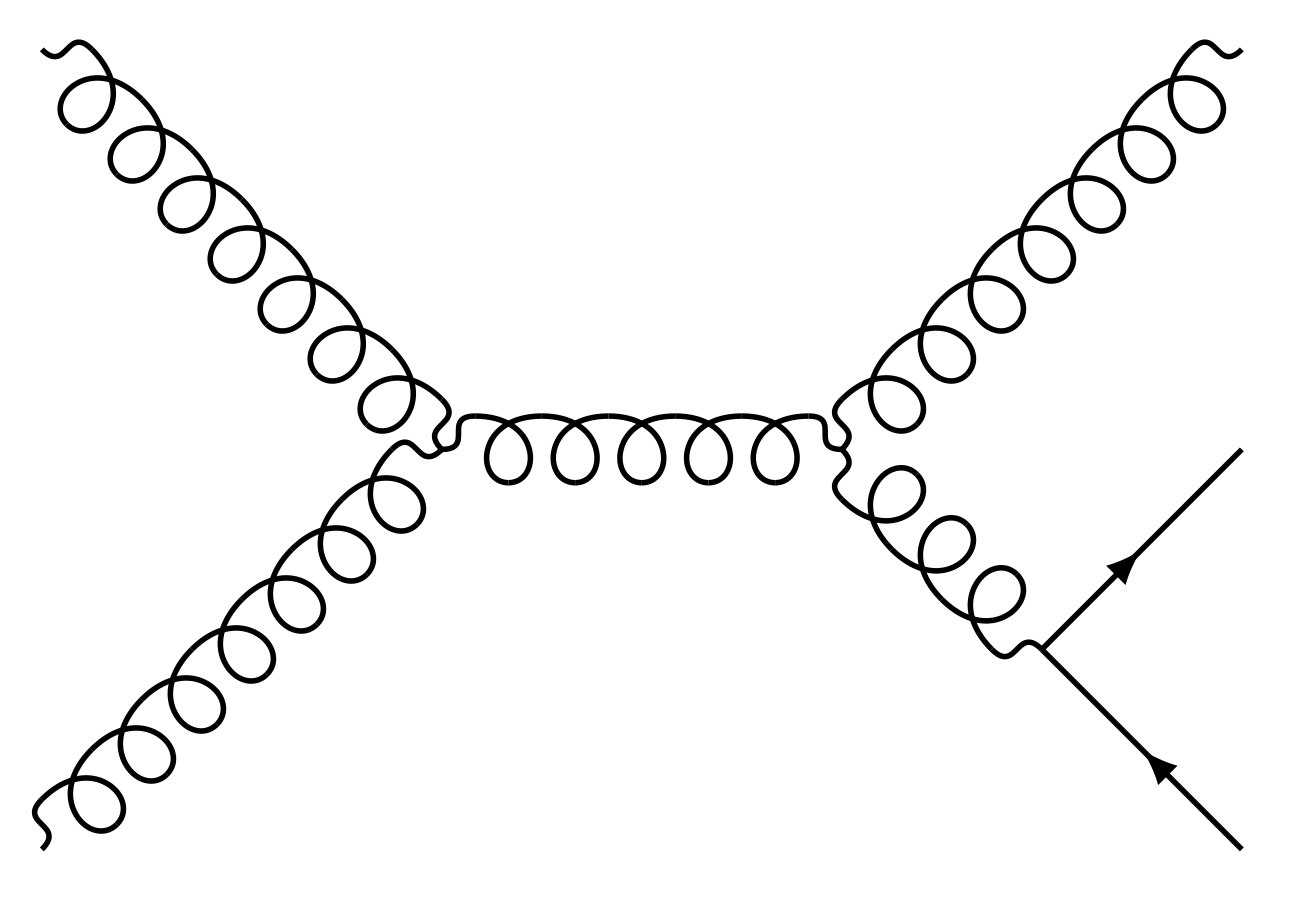
\includegraphics[width=0.3\textwidth]{figures/susy_common/feynman/qcd_3}\label{fig:qcd_prod_3}}
\caption{Representative \gls{lo} Feynman diagram for multijet production. \subref{fig:qcd_prod_1}-\subref{fig:qcd_prod_2} $2 \to 2$ process. 
\subref{fig:qcd_prod_3} $2 \to 3$ process.}\label{fig:qcd_prod}
\end{figure}

\subsubsection*{Jet smearing}
\label{sec:jet_smearing}

The usage of \gls{mc} simulation to model the multijet background presents two main drawbacks.
First of all, the production cross-section for multijet production is very difficult to predict accurately. 
It is feasible to model the $2 \to 2$ di-jet production, 
but every additional parton in a $2 \to n$ process brings into the computation a further $\alpha_{\rm{s}}$ factor, 
and the energy scale of the interaction is low enough to be at the limit of the validity of the perturbative expansion, limiting the validity of a  \gls{lo} order computation. The inclusion of corrections of higher order can improve the description, but the number of extra diagrams that should be included makes this option unrealistic (just the \gls{lo} computation for the $2 \to 2$ process only comprises 10 different diagrams).
A second problem is of practical nature: the high cross-section for multijet production implies a huge number of \gls{mc} events that need to be simulated in order not to have a huge statistical uncertainty. 

The jet smearing method overcomes these problems by providing a data-driven estimate of the multijet background, through the following steps:
\begin{itemize}
\item A sample of well-measured multijet seed events, with low values of \met, is selected in data.

\item Each jet in each seed event is smeared: its four-momentum is multiplied by a random number thrown based on the jet response function, that quantifies the fluctuations in the \pt reconstruction of the jets. The response, defined as the ratio E$_{\rm{T}}^{\rm{reco}}$/E$_{\rm{T}}^{\rm{truth}}$, is determined from \gls{mc} simulations and is then corrected to match data measurements. 
A different response function is used for $b$-tagged jets. 

\item The smearing procedure is repeated a large number of times, $\mathcal{O}(1000)$, for each event, and every time \met is recomputed with the smeared jets as input; some of these smeared events will have high \met values and will satisfy the analysis selections.

\item The number of events that satisfy the analysis selections is arbitrary and depends on the choice of the seed events and on the number of smears for each event. The normalization is derived in a specifically designed \gls{qcd} \gls{cr}, that relies on a tight upper selection on \dphimin ($\dphimin < 0.1$). All the zero-lepton analysis regions have the requirement $\dphimin > 0.4$, which makes them orthogonal to the \gls{qcd} \gls{cr} and allows also to have \glspl{vr} in the intermediate region. 
\end{itemize}

Figure \ref{fig:jet_smear_dphi} shows the distribution of \dphimin in a selection requiring at least four jets, at least two $b$-jets, $\met>200$ GeV and exactly zero lepton. The first bin of this distribution is the region used for the normalization of the multijet background, 
while the phase space up to $\dphimin=0.4$ (which is the lower threshold for the analysis regions) serves as validation region. 
Figures \ref{fig:jet_smear_met} and \ref{fig:jet_smear_jetn} show respectively the distribution of \met and of the number of jets in the \gls{qcd} \gls{cr} and in a validation region with $0.1 < \dphimin < 0.2$.

\begin{figure}[h!]
\centering 
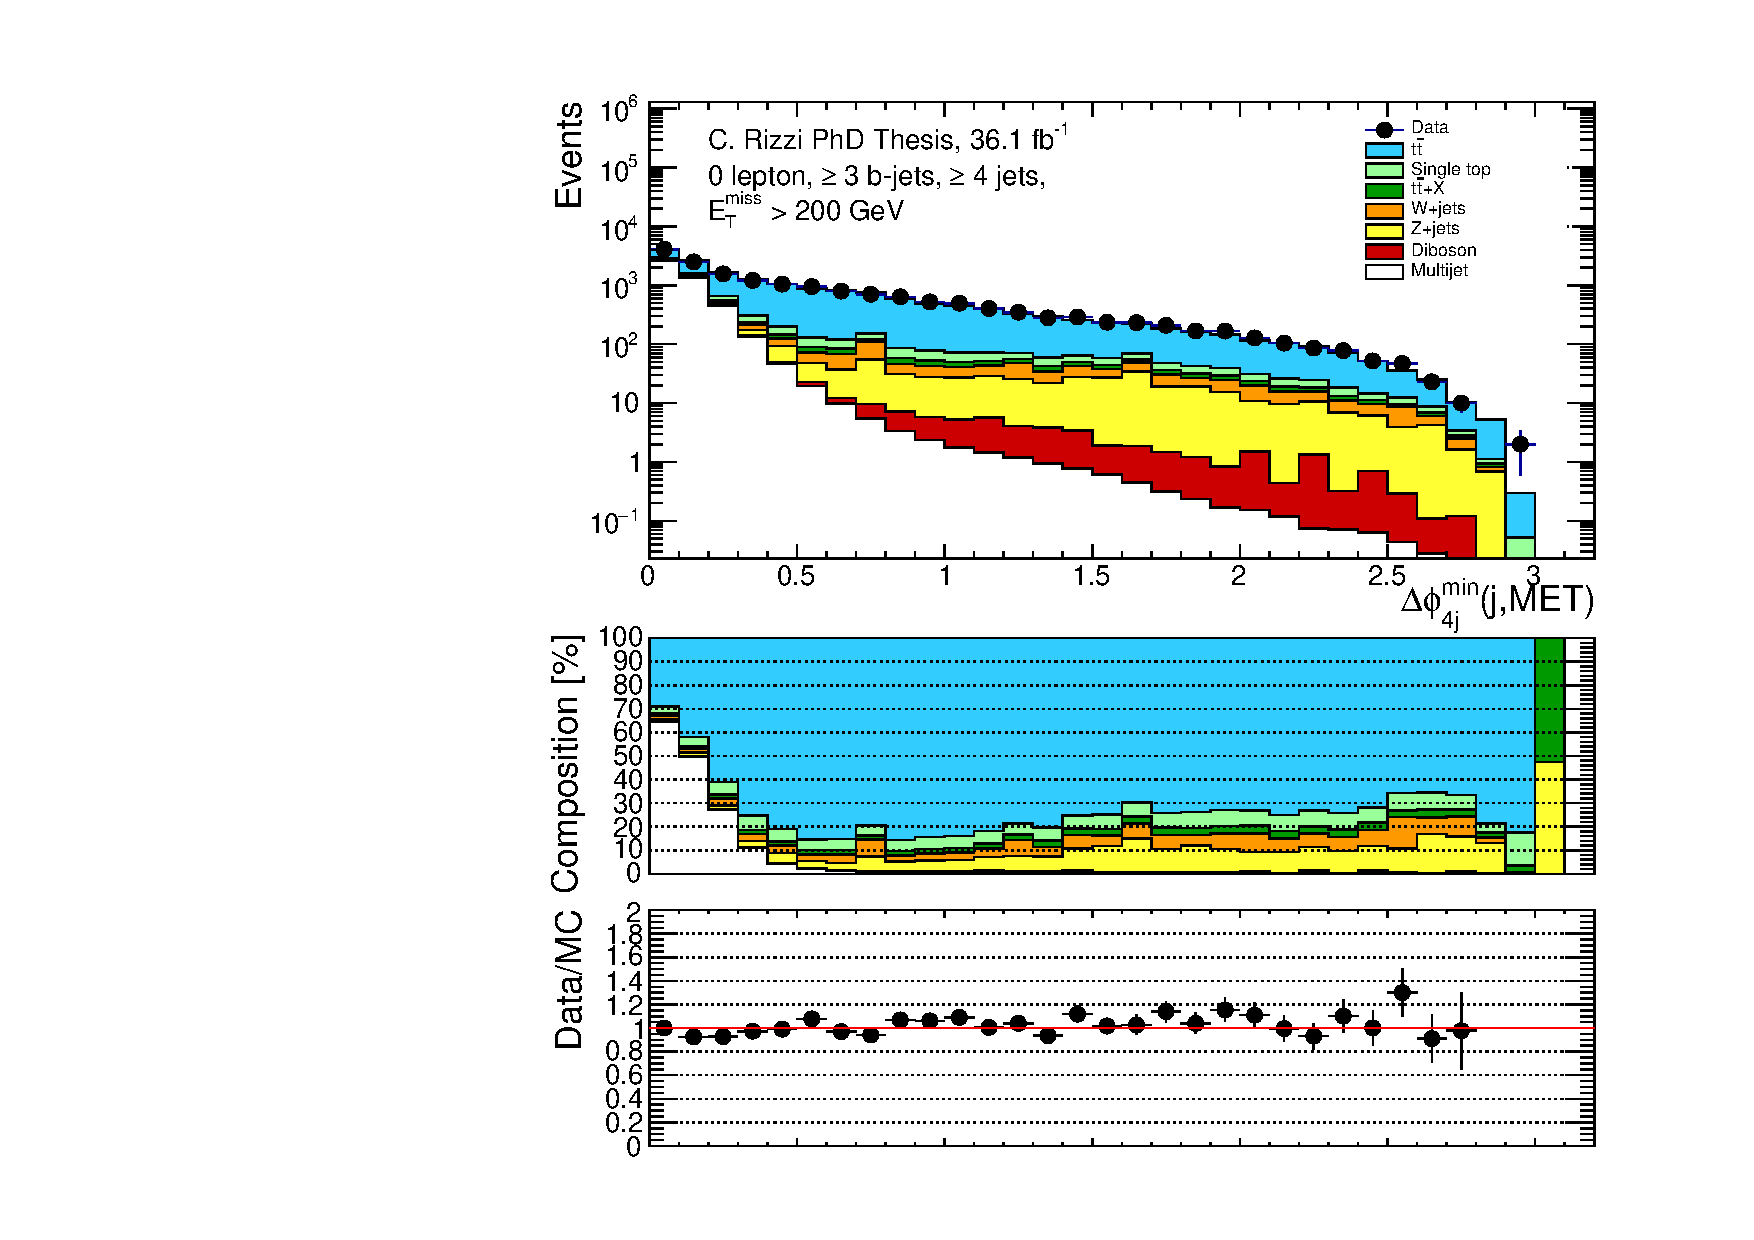
\includegraphics[width=0.49\textwidth]{figures/susy_common/jet_smearing/data_mc_dphi_min_QCD_noDphi.pdf}
\caption{Distribution of \dphimin in a selection requiring at least four jets, at least two $b$-jets, $\met>200$ GeV and exactly zero lepton.}\label{fig:jet_smear_dphi}
\end{figure}


\begin{figure}[h!]
\centering 
\subfigure[]{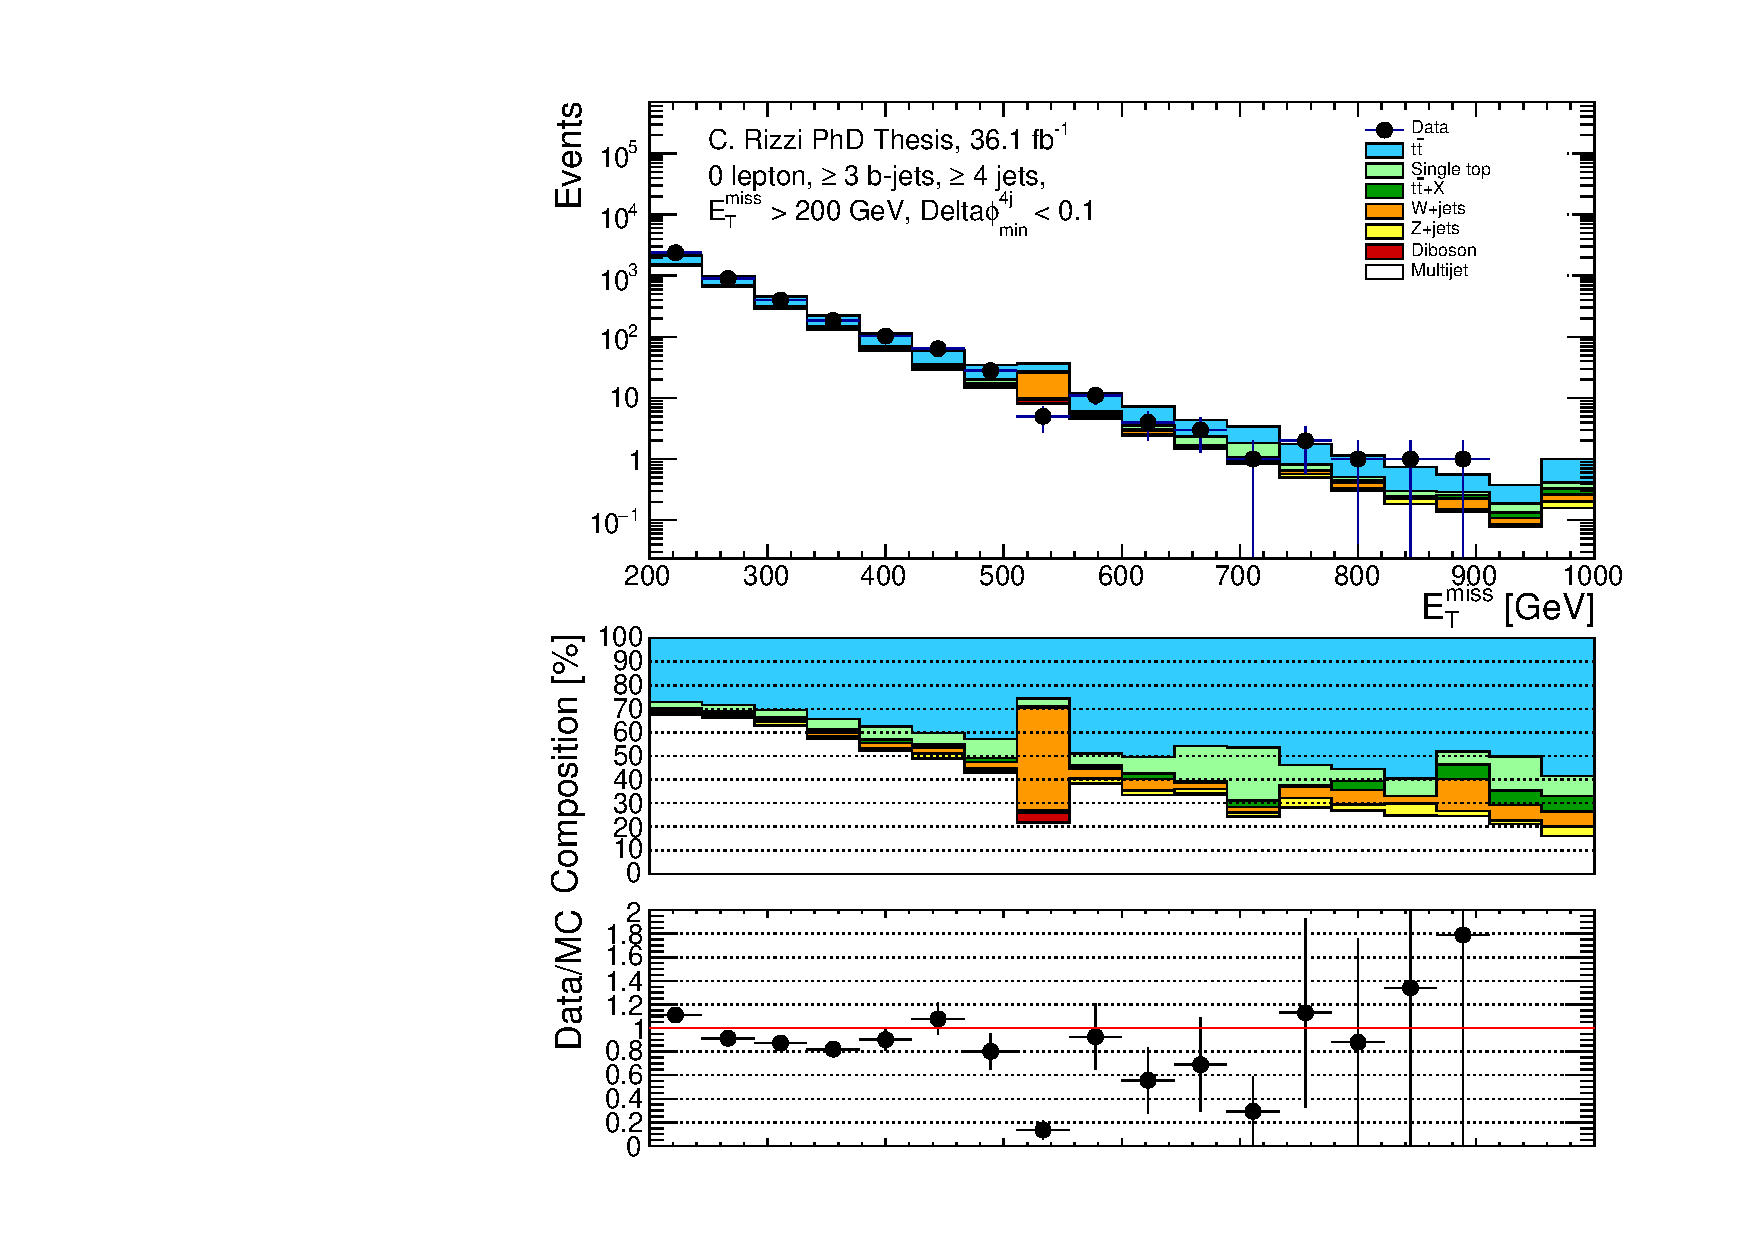
\includegraphics[width=0.49\textwidth]{figures/susy_common/jet_smearing/data_mc_met_QCD_CR.pdf}\label{fig:jet_smear_met_CR}}
\subfigure[]{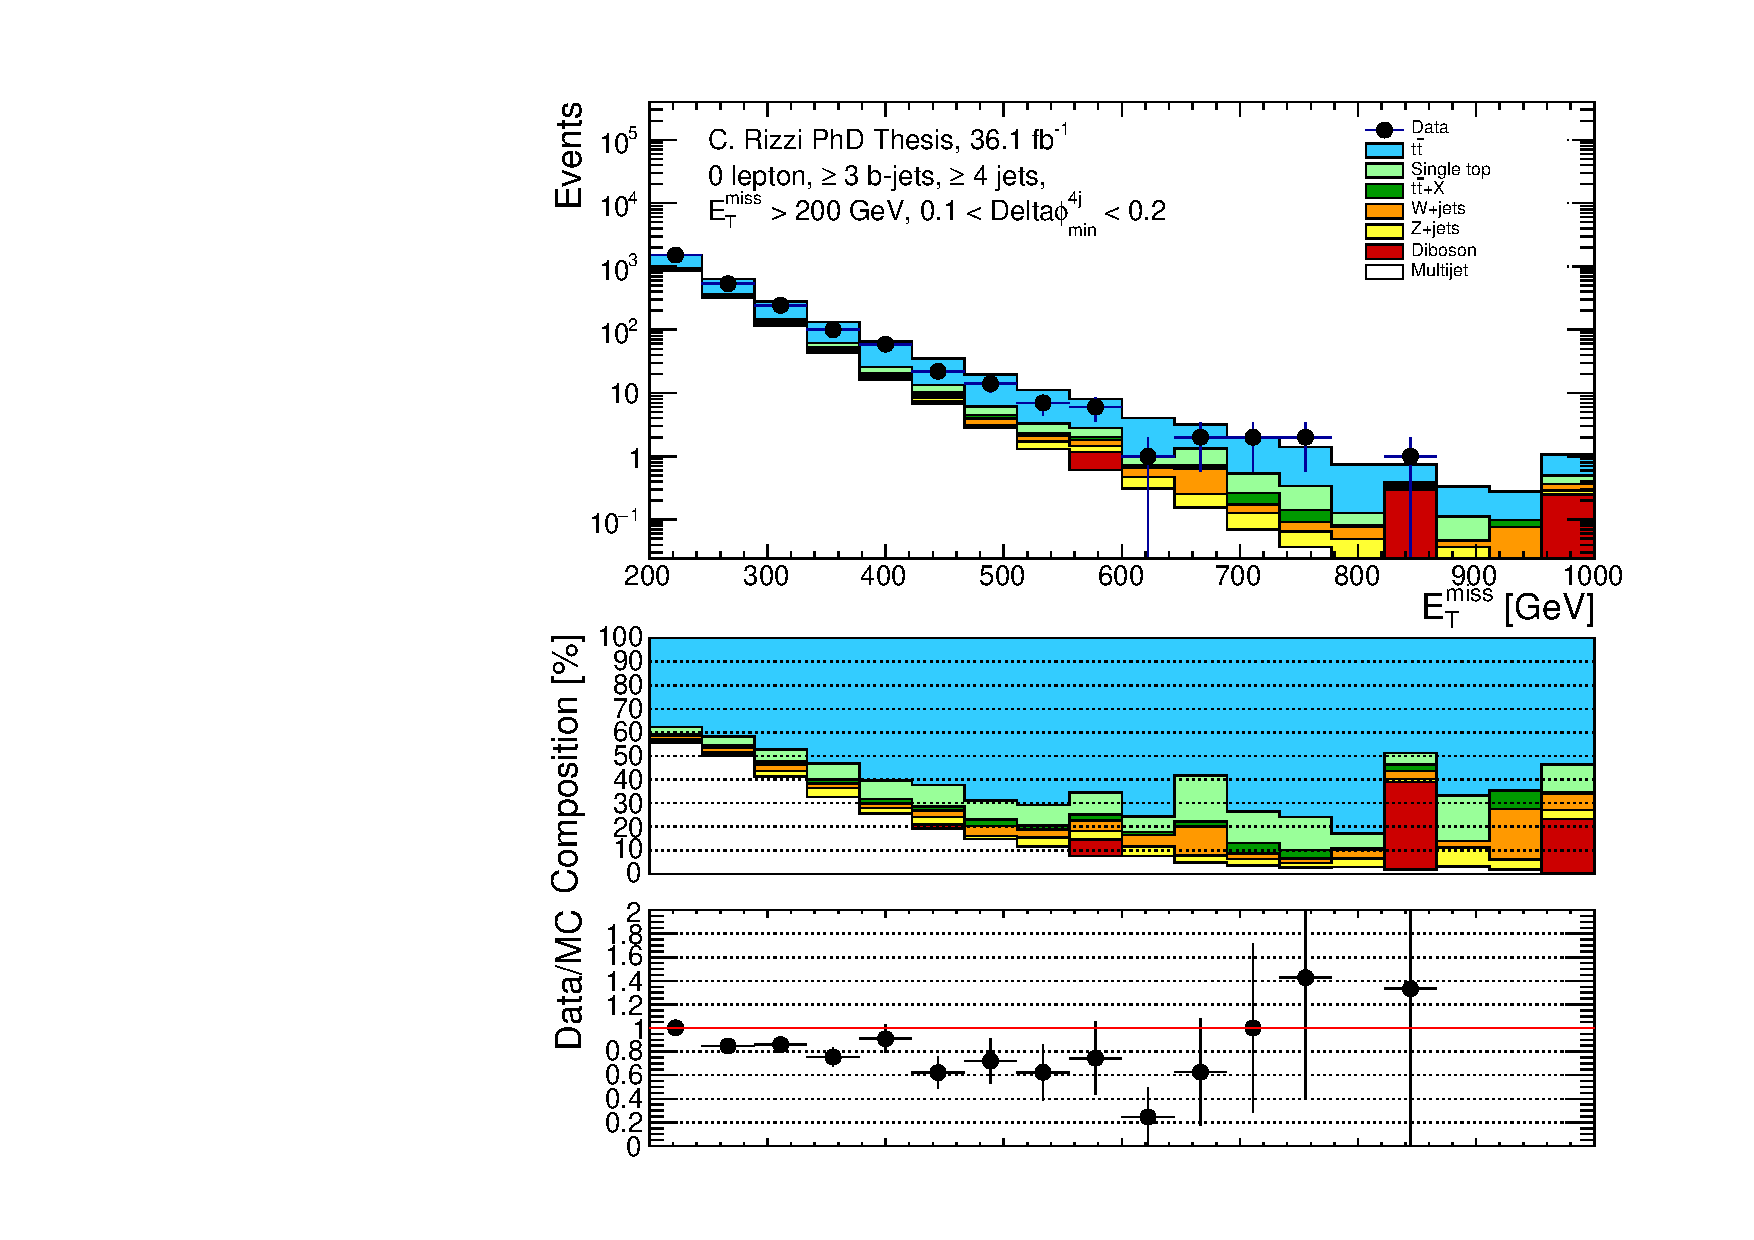
\includegraphics[width=0.49\textwidth]{figures/susy_common/jet_smearing/data_mc_met_QCD_VR1.pdf}\label{fig:jet_smear_met_VR1}}
\caption{Distribution of \met in \subref{fig:jet_smear_met_CR} the region with $\dphimin < 0.1$ where the data-driven estimate for the multijet background is normalized and \subref{fig:jet_smear_met_VR1} the multijet validation region with $0.1 < \dphimin < 0.2$}\label{fig:jet_smear_met}
\end{figure}

\begin{figure}[h!]
\centering 
\subfigure[]{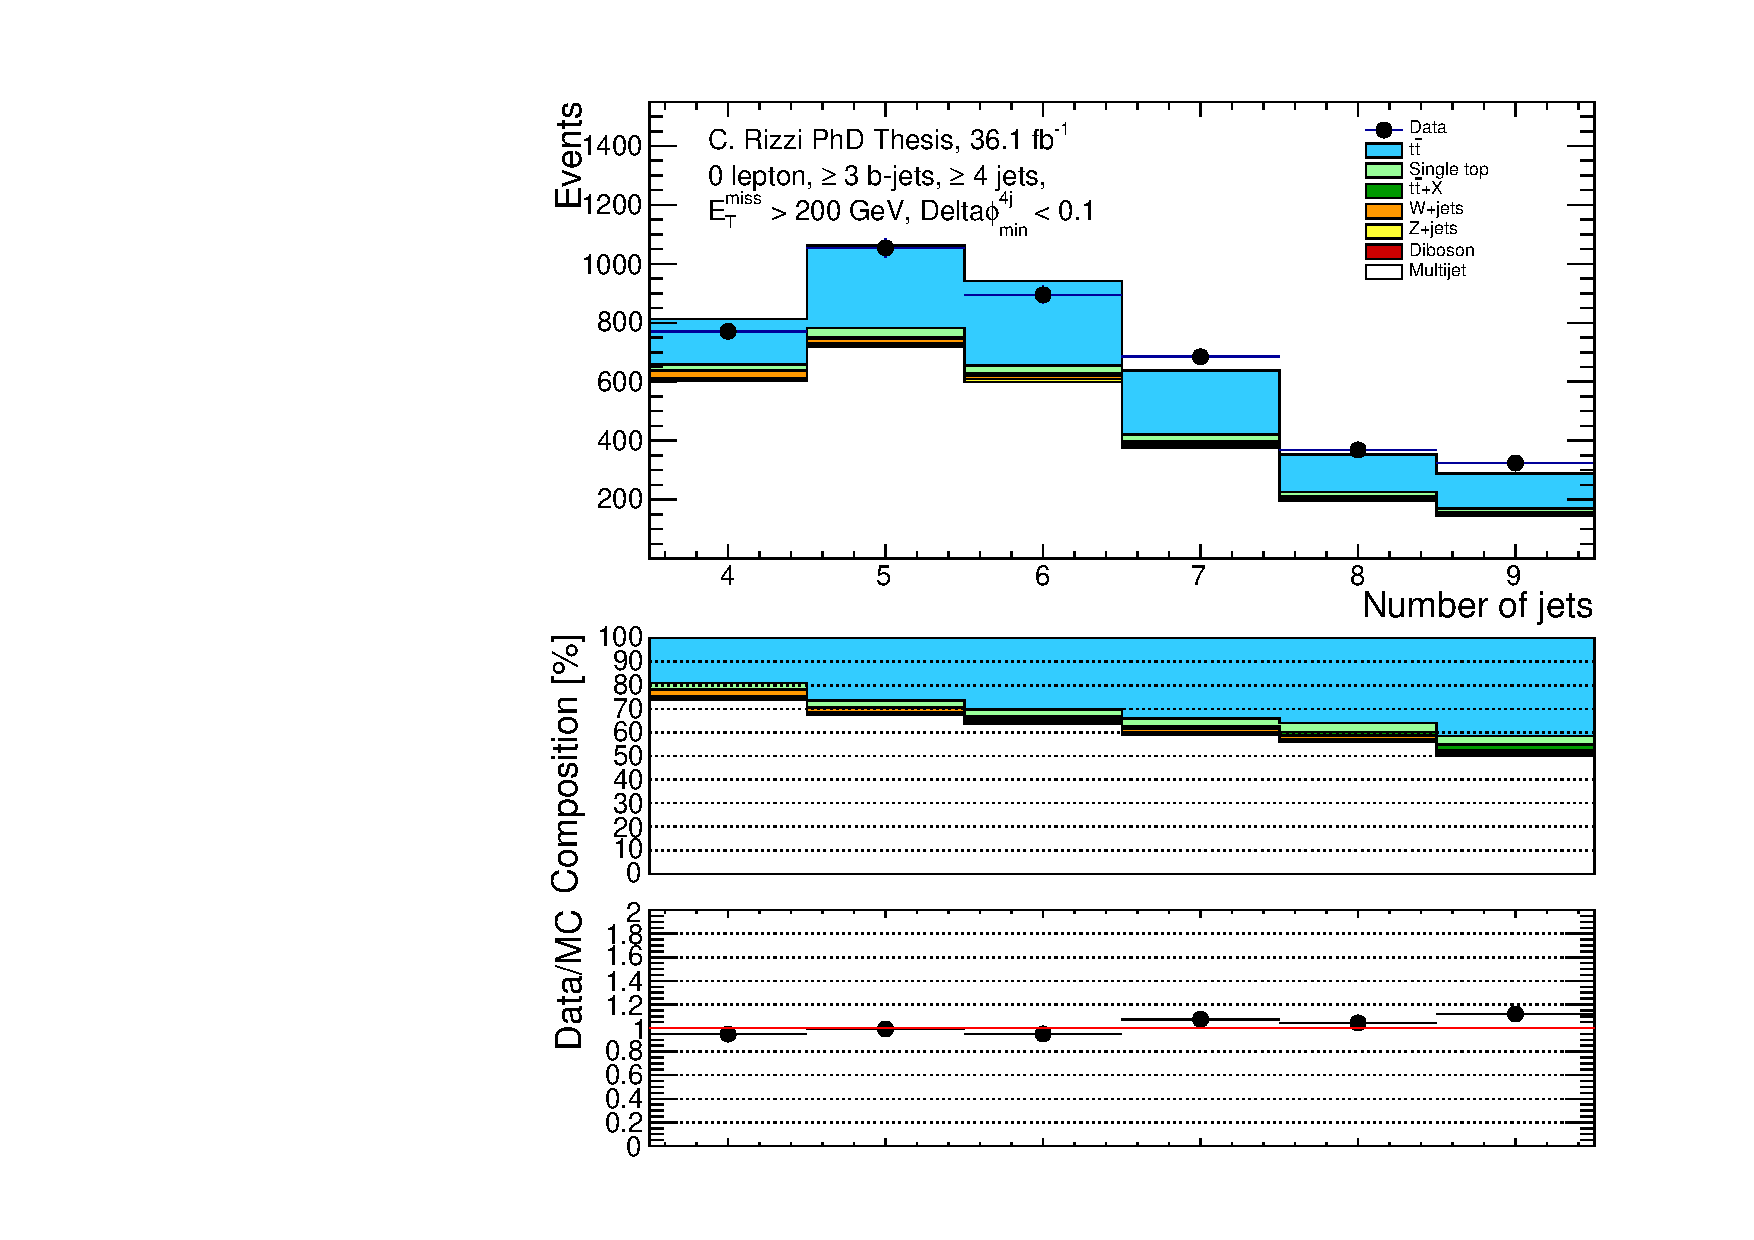
\includegraphics[width=0.49\textwidth]{figures/susy_common/jet_smearing/data_mc_jets_n_QCD_CR.pdf}\label{fig:jet_smear_jetn_CR}}
\subfigure[]{\includegraphics[width=0.49\textwidth]{figures/susy_common/jet_smearing/data_mc_jets_n_QCD_VR1.pdf}\label{fig:jet_smear_jetn_VR1}}
\caption{Distribution of the number of signal jets in \subref{fig:jet_smear_jetn_CR} the region with $\dphimin < 0.1$ where the data-driven estimate for the multijet background is normalized and \subref{fig:jet_smear_jetn_VR1} the multijet validation region with $0.1 < \dphimin < 0.2$}\label{fig:jet_smear_jetn}
\end{figure} 


